% This LaTeX document needs to be compiled with XeLaTeX.
\documentclass[10pt]{article}
\usepackage[utf8]{inputenc}
\usepackage{ucharclasses}
\usepackage{graphicx}
\usepackage[export]{adjustbox}
\graphicspath{ {./images/} }
\usepackage{amsmath}
\usepackage{amsfonts}
\usepackage{amssymb}
\usepackage[version=4]{mhchem}
\usepackage{stmaryrd}
\usepackage{hyperref}
\hypersetup{colorlinks=true, linkcolor=blue, filecolor=magenta, urlcolor=cyan,}
\urlstyle{same}
\usepackage[fallback]{xeCJK}
\usepackage{polyglossia}
\usepackage{fontspec}
\usepackage{newunicodechar}
\setCJKmainfont{Noto Serif CJK SC}

\setmainlanguage{english}
\setotherlanguages{hindi}
\newfontfamily\hindifont{Noto Serif Devanagari}
\newfontfamily\lgcfont{CMU Serif}
\setDefaultTransitions{\lgcfont}{}
\setTransitionsFor{Hindi}{\hindifont}{\lgcfont}

%New command to display footnote whose markers will always be hidden
\let\svthefootnote\thefootnote
\newcommand\blfootnotetext[1]{%
  \let\thefootnote\relax\footnote{#1}%
  \addtocounter{footnote}{-1}%
  \let\thefootnote\svthefootnote%
}

%Overriding the \footnotetext command to hide the marker if its value is `0`
\let\svfootnotetext\footnotetext
\renewcommand\footnotetext[2][?]{%
  \if\relax#1\relax%
    \ifnum\value{footnote}=0\blfootnotetext{#2}\else\svfootnotetext{#2}\fi%
  \else%
    \if?#1\ifnum\value{footnote}=0\blfootnotetext{#2}\else\svfootnotetext{#2}\fi%
    \else\svfootnotetext[#1]{#2}\fi%
  \fi
}

\def\Perp{\perp\!\!\!\perp}

\newunicodechar{×}{\ifmmode\times\else{$\times$}\fi}

\begin{document}
数学奥林匹克小丛书嘪二版 (4) (1) है

初中卷\\
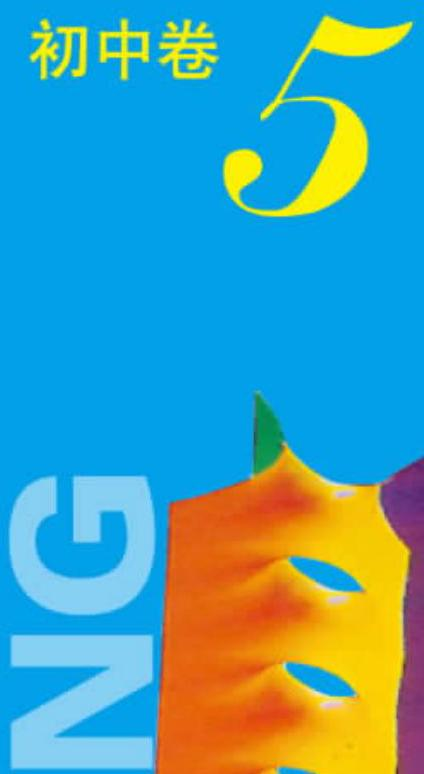
\includegraphics[max width=\textwidth, center]{2024_10_30_66b8e5e701da2093c133g-001}\\
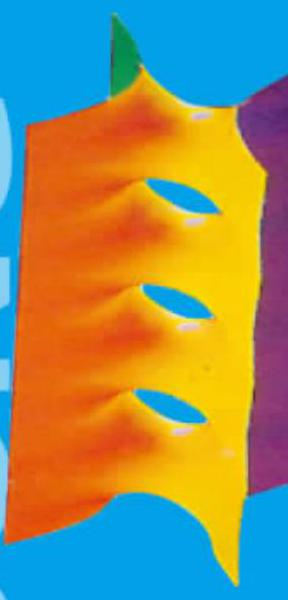
\includegraphics[max width=\textwidth, center]{2024_10_30_66b8e5e701da2093c133g-001(1)}\\
(D)\\
( $)$\\

\includegraphics[max width=\textwidth, center]{2024_10_30_66b8e5e701da2093c133g-001(2)}

是\\
柯新立 编著

数学奥林匹克小丛书\\

\includegraphics[max width=\textwidth, center]{2024_10_30_66b8e5e701da2093c133g-002(1)}

初中卷\\
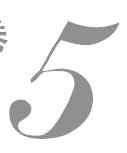
\includegraphics[max width=\textwidth, center]{2024_10_30_66b8e5e701da2093c133g-002}\\

\includegraphics[max width=\textwidth, center]{2024_10_30_66b8e5e701da2093c133g-002(3)}\\

\includegraphics[max width=\textwidth, center]{2024_10_30_66b8e5e701da2093c133g-002(2)}\\
圆\\
柯新立 编著

\section*{图书在版编目(CIP)数据}
圆/柯新立编著. -2 版.一上海:华东师范大学出版社,2012. 2\\
(数学奥林匹克小丛书. 初中卷)\\
ISBN 978-7-5617-9323-7\\
I . (1)圆… II. (1)柯… III. (1) 几何课一初中一教学参考资料 IV. (1)G634. 633

中国版本图书馆 CIP 数据核字(2012)第 027752 号

数学奥林匹克小丛书(第二版) - 初中卷\\
圆

\begin{center}
\begin{tabular}{|c|c|}
\hline
编 著 & 柯新立 \\
\hline
总策划 & 倪 明 \\
\hline
项目编辑 & 孔令志 \\
\hline
审读编辑 & 朱洪敏 \\
\hline
装帧设计 & 高 山 \\
\hline
责任发行 & 郑海兰 \\
\hline
出版发行 & 华东师范大学出版社 \\
\hline
社 址 & 上海市中山北路3663号 邮编200062 \\
\hline
网 址 & www. ecnupress. com.cn \\
\hline
电 话 & 021-60821666 行政传真 021-62572105 \\
\hline
客服电话 & 021-62865537 门市(邮购) 电话021-62869887 \\
\hline
地 址 & 上海市中山北路 3663 号华东师范大学校内先锋路口 \\
\hline
 & http://hdsdcbs. tmall. com \\
\hline
\end{tabular}
\end{center}

印刷者 浙江省临安市曙光印务有限公司\\
开 本 787×1092 16开\\
插 页 1\\
印 张 6.75\\
字 数 114 千字\\
版 次 2012 年 7月第一版\\
印 次 2012 年 7月第一次\\
印 数 1-13000\\
书 号 ISBN 978-7-5617-9323-7/G $\cdot$ 5577\\
定 价 15.00 元\\
出版 人 朱杰人

\section*{数学奥林匹克小丛书(第二版)编委会}
冯志刚 第53届IMO中国队副领队、上海中学特级教师\\
葛 军 博士、中国数学奥林匹克高级教练、南京师范大学副教授江苏省中学数学教学研究会副理事长\\
冷岗松 国家集训队教练、上海大学教授、博士生导师\\
李胜宏 第44届IMO中国队领队、浙江大学教授、博士生导师\\
李伟固 中国数学奥林匹克委员会委员、国家集训队教练北京大学教授、博士生导师\\
刘诗雄 华南师范大学中山附属中学校长、中学数学特级教师\\
倪 明 华东师范大学出版社教辅分社社长、编审\\
单 墫 第30、31届IMO中国队领队、南京师范大学教授、博士生导师\\
吴建平 中国数学会普及工作委员会主任、中国数学奥林匹克委员会副主席\\
熊 斌 第46、49、51、52、53届IMO中国队领队\\
中国数学奥林匹克委员会委员、华东师范大学教授、博士生导师\\
余红兵 中国数学奥林匹克委员会委员、国家集训队教练苏州大学教授、博士生导师\\
朱华伟 中国教育数学学会常务副理事长、国家集训队教练\\
广州大学软件所所长、研究员

\section*{心}
\begin{center}
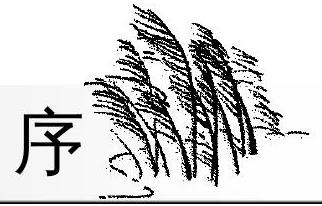
\includegraphics[max width=\textwidth]{2024_10_30_66b8e5e701da2093c133g-006}
\end{center}

数学竞赛像其他竞赛活动一样,是青少年学生的一种智力竞赛。在类似的以基础科学为竞赛内容的智力竞赛活动中,数学竞赛的历史最悠久、国际性强,影响也最大。我国于1956年开始举行数学竞赛,当时最有威望的著名数学家华罗庚、苏步青、江泽涵等都积极参加领导和组织竞赛活动,并组织出版了一系列青少年数学读物,激励了一大批青年学生立志从事科学事业。我国于1986年起参加国际数学奥林匹克,多次获得团体总分第一,并于1990年在北京成功地举办了第 31 届国际数学奥林匹克,这标志着我国数学竞赛水平在国际上居领先地位,为各国科学家与教育家所瞩目。

我国数学竞赛活动表明,凡是开展好的地区和单位,都能大大激发学生的学习数学的兴趣,有利于培养创造性思维,提高学生的学习效率。这项竞赛活动,将健康的竞争机制引进数学教学过程中,有利于选拔人才。由数学竞赛选拔的优胜者,既有踏实广泛的数学基础,又有刻苦钻研、科学的学习方法,其中的不少青年学生将来会成为出色的科学工作者。在美国,数学竞赛的优胜者中后来成名如米尔诺(J. W. Milnor)、芒福德(D. B. Mumford)、奎伦 (D. Quillen)等都是菲尔兹数学奖的获得者;在波兰,著名数论专家辛哲尔 (A. Schinzel)学生时代是一位数学竞赛优胜者;在匈牙利,著名数学家费叶尔 (L. Fejér)、里斯(M. Riesz)、舍贵(G. Szegö)、哈尔(A. Haar)、拉多 (T. Radó)等都曾是数学竞赛获奖者。匈牙利是开展数学竞赛活动最早的国家,产生了同它的人口不成比例的许多大数学家!

在开展数学竞赛的活动同时,各学校能加强联系,彼此交流数学教学经验,从这种意义上来说,数学竞赛可能成为数学课程改革的"催化剂",成为培养优秀人才的有力措施。

不过,应当注意在数学竞赛活动中,注意普及与提高相结合,而且要以普及为主,使竞赛具有广泛的群众基础,否则难以持久。

当然,现在有些人过于关注数学竞赛的成绩,组织和参与都具有很强的功利目的,过分扩大数学竞赛的作用,这些都是不正确的,违背了开展数学竞赛活动的本意。这些缺点有其深层次的社会原因,需要逐步加以克服,不必因

为有某些缺点,就否定这项活动。\\
我十分高兴看到这套《数学奥林匹克小丛书》的正式出版。这套书,规模大、专题细。据我所知,这样的丛书还不多见。这套书不仅对数学竞赛中出现的常用方法作了阐述,而且对竞赛题作了精到的分析解答,不少出自作者自己的研究所得, 是一套很好的数学竞赛专题教程, 也是中小学生和教师的参考书。

这套小丛书的作者都是数学竞赛教学和研究人员,不少是国家集训队的教练和国家队的领队。他们为我国开展数学竞赛的活动和我国学生在 IMO 上取得成绩、为国争光作出了贡献,为这套书尽早面世付出了艰辛的劳动。华东师大出版社在出版《奥数教程》和《走向 IMO》等竞赛图书基础上,策划组织了这套丛书,花了不少心血。我非常感谢作者们和编辑们在这方面所做的工作,并衷心祝愿我国的数学竞赛活动开展得越来越好。

\section*{五元}
\footnotetext{王元,著名数学家,中国科学院院士,曾任中国数学会理事长、中国数学奥林匹克委员会主席.
}
1 圆、扇形、弓形的周长和面积 ..... 001\\
2 圆的对称性 ..... 007\\
3 与圆有关的角 ..... 012\\
4 与圆相关的位置关系 ..... 019\\
5 圆的切线 ..... 024\\
6 四点共圆 ..... 033\\
7 圆幂定理 ..... 042\\
8 圆的幂及应用 ..... 048\\
9 托勒密定理及其应用 ..... 055\\
10 三角形的外心与内心 ..... 061\\
11 与圆有关的杂题 ..... 070\\
习题解答 ..... 075

\section*{华东师大精品奥数图书}
\section*{学奥数,这里总有一本适合你}
"奥数"入门篇——《课本到奥数》(1-9 年级)本书或许不适合你,如果你\\
A. 每次考试都能超过 95 分-so easy!\\
B. 考试很少能超过 80 分一so difficult!\\
C. 不认为自己能学好数学一 Attitude first!

读者对象:数学成绩班级前 $5 \%-30 \%$ 的优等生\\
"奥数"智优篇——《优等生数学》(1-9 年级)\\
如果说"奥数"是提供给 $4 \%$ 的优等生,\\
那么《优等生数学》提供给 $20 \%$ 的优等生。\\
如果你已经是优等生,不妨一读;\\
如果你想成为优等生,不能不读!\\
读者对象:数学成绩班级前 $20 \%$ 的优等生\\
"奥数"辅导篇——《奥数教程》、《学习手册》、《能力测试》

\begin{itemize}
  \item 第十届全国教育图书展优秀畅销图书
  \item 国家集训队教练执笔联合编写
  \item 在香港出版繁体字版和网络版
  \item 2010 年最新修订,三本配套使用,效果更佳
\end{itemize}

读者对象:数学成绩班级前 $10 \%$ 的优等生、竞赛教练员\\
"奥数"题库篇——《多功能题典》初中、高中数学竞赛

\begin{itemize}
  \item 题量大、内容全、解法精
  \item 分类细:按照章节、难度、题型、方法等维度分类
  \item 配有网络检索功能 \href{http://tidian}{http://tidian}. ecnupress. com. cn读者对象:成绩优秀的中学生、竞赛教练员、数学爱好者\\
"奥数"课外阅读篇——《单墫老师教你学数学》 7 种\\
当读书不只是为了考试\\
你才会真正爱上数学\\
单墫老师妮娓道来\\
与你分享他所理解的数学之美\\
读者对象:初高中学生,数学教师,数学爱好者\\
"奥数"域外篇——《全俄中学生数学奥林匹克(1993-2006)》\\
俄罗斯是世界上开展数学活动最早、最广泛、也是影响最大的国家之一。俄罗斯是世界上竞赛试题的最大生产国,不仅产量高,而且质量好,其中最出色的当数组合题。
\end{itemize}

本书收录 1993-2006年俄罗斯 9-11年级数学奥林匹克第四轮(联邦区域竞赛)和第五轮(全俄决赛)竞赛的所有试题和解答。

读者对象:参加数学竞赛的中学生、竞赛教练员、数学爱好者\\
"奥数"高中预赛篇——《高中数学联赛备考手册(预赛试题集锦)》

\begin{itemize}
  \item 从2009年起,每年出版一册
  \item 收录了当年各省市预赛试题和优秀解答(约 20 份)
  \item 试题在遵循现行教学大纲, 体现新课标精神的同时, 在方法的要求上有所提高
  \item 命题人员大多同时兼任各省市高考命题工作,试题对高考有一定的指导作用\\
读者对象:参加预赛和联赛的高中生、竞赛教练员、高中教师\\
"奥数"联赛冲刺篇——《初(高)中数学联赛考前辅导》
  \item 选题经典且贴近高中联赛
  \item 知识上查漏补缺,能力上全面提升
  \item 全新模拟题让你提前感受考场氛围
\end{itemize}

读者对象:参加联赛的高中生、竞赛教练员、高中教师\\
"奥数"IMO 终极篇——《走向 IMO:数学奥林匹克试题集锦》

\begin{itemize}
  \item 从 2003 年起,每年出版一册
  \item 以国家集训队测试题和国家队训练题为主
  \item 收集了国内主要竞赛:全国联赛、联赛加试、冬令营、女子数学奥林匹克、西部数学奥林匹克、东南地区数学奥林匹克
  \item 附有美国、俄罗斯、罗马尼亚和国际数学奥林匹克
\end{itemize}

读者对象:参加联赛、冬令营等赛事的高中生、竞赛教练员、数学爱好者\\
更多图书信息及免费资料请登录:\\
\href{http://www}{http://www}. hdsdjf. com/downloadfileinfor. aspx? classid=69

\section*{圆、扇形、弓形的周长和面积}
平面上到定点距离等于定长的点的集合称为圆。\\
扇形、弓形都是圆的一部分。圆中一段弧及过该弧两端点的半径围成的图形称为扇形;由圆的弦及所对弧围成的图形称为弓形。

设圆的半径为 $r$, 则圆的周长 $C=2 \pi r$, 面积 $S=\pi r^{2}$.\\
若扇形的半径为 $r$, 弧所对圆心角为 $n^{\circ}$, 则扇形弧长 $l=\frac{n \pi r}{180}$, 扇形周长 $C=\frac{n}{180} \pi r+2 r$ ,面积 $S=\frac{n \pi r^{2}}{360}$.

弓形面积则需考虑弦所对弧是优弧还是劣弧。如图\\
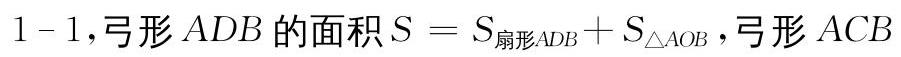
\includegraphics[max width=\textwidth]{2024_10_30_66b8e5e701da2093c133g-011(1)}的面积 $S=S_{\text {扇形 } A C B}-S_{\triangle A O B}$ ,弓形的周长 $C=$ 弦长 + 弧长。

由圆、扇形、弓形等构成的组合图形面积或周长计算通常需一定技巧,常见处理这类问题的手段是分解组合、\\
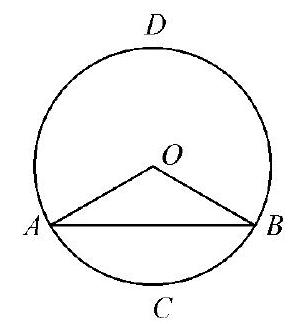
\includegraphics[max width=\textwidth, center]{2024_10_30_66b8e5e701da2093c133g-011(2)}

图1-1

等积变形等等。

例1 如图 1-2, $A B 、 C D$ 是 $\odot O$ 的两条互相垂直的直径,且 $A B=2$ ,以点 $B$ 为圆心, $B A$ 为半径画弧 $\overparen{A E}$ 交 $C D$ 延长线于点 $E$, 又四边形 $E F G O$ 为正方形,求阴影部分的面积。

分析 将图形分割为 $A E D$ 区域和 $D E F G B$ 区域,其中 $A E D$ 区域的面积等于扇形 $A B E$ 的面积减去扇形 $A O D$ 的面积及 $\triangle O B E$ 的面积之和。

解 注意到 $B A=B E$ ,且 $E O$ 垂直平分 $A B$ ,故\\
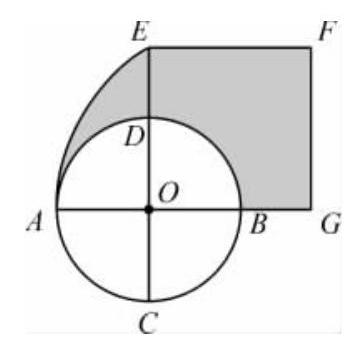
\includegraphics[max width=\textwidth, center]{2024_10_30_66b8e5e701da2093c133g-011}

图1-2\\
$\triangle A B E$ 为正三角形, $\angle A B E=60^{\circ}, O E=\frac{\sqrt{3}}{2} A B=\sqrt{3}$, 所以

\begin{align*}
S_{\text {阴ADE }}=S_{\text {扇形 } A B E}-S_{\text {扇形 } A O D}-S_{\triangle O B E}
\end{align*}

1 圆、扇形、弓形的周长和面积

易知 $\triangle O F M \cong \triangle I O N$ ,从而 $S_{Q N M F}=S_{I Q O}$ ,而区域 $I H G F Q$ 为公共部分,故 $S_{\text {扇形 } 1 O F}=S_{F M N I}$ 。

又 $\triangle G J O \cong \triangle O K H$ ,所以 $S_{G P K J}=S_{O H P}$ 又区域 $G H P$ 为公共部分,故 $S_{G H K J}=S_{\text {扇形HOG }}$.

从而在区域 FMNI 中,

\begin{align*}
\begin{aligned}
S_{\text {阴 }} & =S_{\text {扇形IOF }}-S_{\text {扇形 } H O G ~} \\
& =S_{\text {扇形IOG }} \\
& =\frac{36}{360} \pi r^{2} \\
& =40 \pi .
\end{aligned}
\end{align*}

由于对称性,于是在区域 $A I F D$ 中, $S_{\text {阴 }}=80 \pi$.\\
例 4 在一个三边长分别为 $50 、 120 、 130$ 的三角形内部和外部分别取与三角形边上至少有一点的距离为 2 的所有点, 求所有这些点构成的区域的面积。

解 依题意,所求面积区域为图 1 - 5 中 $\triangle A_{1} B_{1} C_{1}$ 的外围部分面积。\\
$\triangle A B C$ 的三个顶点处各有一个小扇形,半径均为 2 ,合在一起恰为一个半径为 2 的圆,故图中 $\triangle A C B$ 外部面积 $S_{1}=\pi \times 2^{2}+(50+120+$ 130) $\times 2=600+4 \pi$.\\
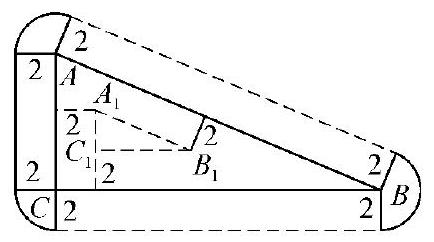
\includegraphics[max width=\textwidth, center]{2024_10_30_66b8e5e701da2093c133g-013}

图 1-5

其次, 易知 $\triangle A_{1} C_{1} B_{1} \backsim \triangle A C B$, 且共内心, 内切圆半径相差 2 . 由于 $\triangle A C B$ 的内切圆半径为 $\frac{50+120-130}{2}=20$ ,故 $\triangle A_{1} B_{1} C_{1}$ 的内切圆半径为 18 。

所以

\begin{align*}
\frac{S_{A_{1} B_{1} C_{1}}}{S_{A B C}}=\frac{81}{100}
\end{align*}

从而

\begin{align*}
\begin{aligned}
S_{A_{1} B_{1} C_{1}} & =\frac{81}{100} \times S_{A B C} \\
& =\frac{81}{100} \times \frac{1}{2} \times 50 \times 120 \\
& =2430
\end{aligned}
\end{align*}

于是夹在 $\triangle A_{1} B_{1} C_{1}$ 与 $\triangle A B C$ 之间的区域面积 $S_{2}$ 为 570 .\\
所以符合条件的点构成区域的面积等于 $S_{1}+S_{2}=600+4 \pi+570=$ $1170+4 \pi$.

1 圆、扇形、弓形的周长

例 5 在边长为 1 的正五边形 $A B C D E$ 内,去掉所有与各顶点距离都小于 1 的点, 求余下部分的面积。

分析 关键是确定余下部分的形状。\\
解 如图 1-6所示,分别以点 $A 、 B 、 C 、 D 、 E$为圆心,以 1 为半径画弧,这些弧围成一个"曲边五边形" $M N P Q R$ ,其内部的点到正五边形各顶点的距离都\\
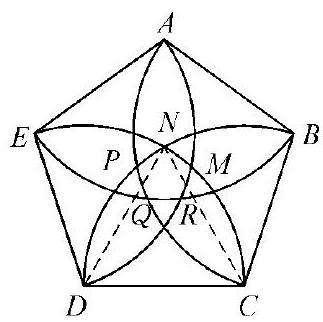
\includegraphics[max width=\textwidth, center]{2024_10_30_66b8e5e701da2093c133g-014}

图1-6

小于 1 ,余下的部分由五个等积的形如"曲边三角形" $N B C$ 的图形组成。

注意到曲边三角形 $N B C$ 与扇形 $N D C$ 的面积之和等于 $\triangle D N C$ 与扇形 $N C B$ 的面积之和,所以所求余下部分的面积

\begin{align*}
\begin{aligned}
S & =5\left(S_{\triangle D N C}+S_{\text {扇形 } N C B}-S_{\text {扇形 } N D C}\right) \\
& =5\left(\frac{\sqrt{3}}{4}+\frac{108-60}{360} \pi-\frac{60}{360} \pi\right) \\
& =\frac{5 \sqrt{3}}{4}-\frac{\pi}{6} .
\end{aligned}
\end{align*}

例 6 已知正方形和三角形都外切于半径为 1 的圆,求证:正方形和三角形重叠部分且在圆的外部区域的面积大于 0.34 。

证明 当三角形的边与正方形的边所在直线不重合或平行时,则三角形的边必将正方形截去一个"角",此"角"在"重叠部分"之外. 先考虑此部分面积的情况。

如图 1-7, $\odot O$ 切正方形的边于点 $E 、 F$ ,切 $\triangle A B C$的边于点 $D$, 连结 $O E 、 O B 、 O D 、 O C 、 O F$ ,则四边形 $O E A F$ 为正方形。

设 $A B=x, A C=y$, 则 $B D=E B=1-x, C D=$ $C F=1-y$, 故在Rt $\triangle A B C$ 中有

\begin{align*}
(1-x+1-y)^{2}=x^{2}+y^{2},
\end{align*}

\begin{center}
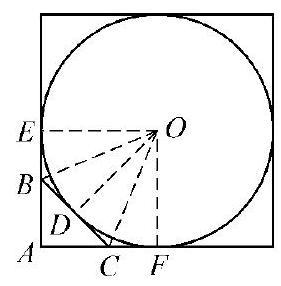
\includegraphics[max width=\textwidth]{2024_10_30_66b8e5e701da2093c133g-014(1)}
\end{center}

图 1-7

化简整理得

\begin{align*}
2+x y=2(x+y)
\end{align*}

于是

\begin{align*}
2+x y=2(x+y) \geqslant 4 \sqrt{x y},
\end{align*}

解得

\begin{align*}
\sqrt{x y} \geqslant 2+\sqrt{2} \text {, 或 } \sqrt{x y} \leqslant 2-\sqrt{2} \text {, }
\end{align*}

但 $0<x 、 y<1$, 从而 $\sqrt{x y}<1$.

于是 $\quad \sqrt{x y} \leqslant 2-\sqrt{2}, S_{\triangle B B C}=\frac{1}{2} x y \leqslant(\sqrt{2}-1)^{2}$.\\
由于三角形的边最多截去正方形三个"角",从而三角形与正方形重叠部分的面积至少为 $S_{\text {正 }}-3 S_{\triangle A B C}$, 若符合题意的区域面积为 $S$, 则

\begin{align*}
\begin{aligned}
S & \geqslant S_{\text {正 }}-3 S_{\triangle A B C}-S_{\text {圆 }} \\
& \geqslant 2^{2}-3 \times(\sqrt{2}-1)^{2}-\pi \times 1^{2} \\
& =6 \sqrt{2}-5-\pi>0.34 .
\end{aligned}
\end{align*}

说明 正方形与三角形重叠部分的面积不可能等于 $6 \sqrt{2}-5$ ,但可无限接近.

\section*{习 题 1}
\begin{enumerate}
  \item Rt $\triangle A B C$ 中, $A C=B C, \angle C=90^{\circ}$, 点 $D$ 在边 $A B$ 上, 以 $A$ 为圆心, $A D$为半径画弧交 $B C$ 于点 $E$, 交 $A C$ 延长线于点 $F$. 若图中两个阴影部分面积相等,求 $A D: D B$ 。\\
2 在一块周长为 500 米的三角形草坪周围修筑一条宽 1 米的小路, 且路的\\
任何一处至少与草坪的某处距离为 1 米,求路的占地面积。\\
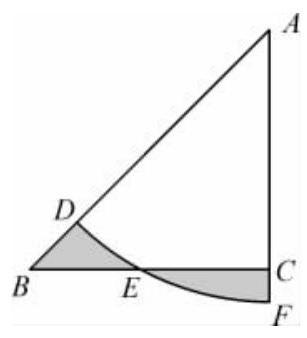
\includegraphics[max width=\textwidth, center]{2024_10_30_66b8e5e701da2093c133g-015(1)}\\
(第1题)\\
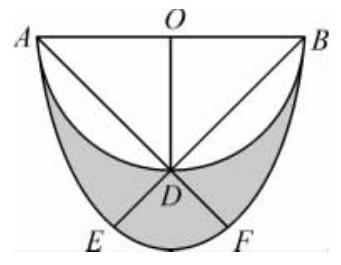
\includegraphics[max width=\textwidth, center]{2024_10_30_66b8e5e701da2093c133g-015}\\
(第3题)
\end{enumerate}

3 . $A B$ 是半圆 $O$ 的直径,作 $O D \perp A B$ 交半圆 $O$ 于点 $D$ ,分别以点 $A 、 B$ 为圆心, $A B$ 为半径画弧交 $A D 、 B D$ 延长线于 $F 、 E$ ,再以点 $D$ 为圆心, $D E$为半径画弧,连接 $E 、 F$ ,若 $A B=2$ ,求图中阴影部分的面积。\\
4 直角三角形 $A C B$ 中, $A C=C B=2, \angle C=90^{\circ}$ ,将 $\triangle A C B$ 绕 $C$ 顺时针转 $90^{\circ}$ ,求边 $A B$ 扫过的区域面积。\\
5 将一枚半径为 1 cm 的硬币置于正 $n$ 边形内,硬币可在里面任意移动,但不可超越边界,求正 $n$ 边形内硬币不能接触到的部分面积。

1 圆、扇形、弓形的周长和面积

6 正三角形的边长为 $a$, 过每两个顶点及中心 $O$ 在三角形内作弧,求阴影部分的面积 $S_{\text {阴。 }}$ 。\\
7 正三角形的边长为 $2 a$, 以各顶点为圆心, $\sqrt{2} a$ 为半径画圆,求:圆的公共部分面积。\\
$8 \triangle A B C$ 的三条边 $A B=c, B C=a, C A=b$ ,作 $\triangle A B C$ 的内切圆,再作此内切圆的三条切线分别平行 $A B 、 B C 、 C A$ ,又得到三个小三角形,再\\
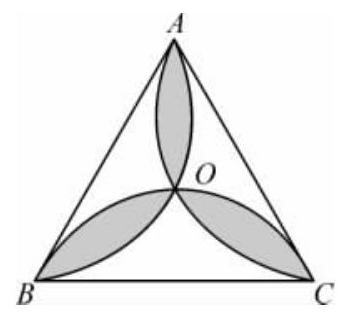
\includegraphics[max width=\textwidth, center]{2024_10_30_66b8e5e701da2093c133g-016}\\
(第 6 题)

作这三个小三角形的内切圆,求这四个圆的面积之和。

平面上到定点距离等于定长的点的集合称为圆. 圆既是轴对称图形,又是中心对称图形. 圆的任意一条直径是圆的对称轴, 圆心是圆的对称中心. 圆的对称性是圆的最基本性质,垂径定理是圆的轴对称性的集中体现。

垂径定理: 垂直于弦的直径平分这条弦, 并且平分弦所对的两条弧.\\
如图 2-1 所示, 直径 $C D$ 垂直于弦 $A B$ 于点 $H$,我们可以得到: $A H=H B ; \overparen{A C}=\overparen{C B} ; \overparen{A D}=\overparen{D B}$ 。

事实上,垂径定理中五个要素:(1)直径(CD),(2)平分弦 $A B$, (3)垂直于弦 $A B$, (4)平分弧 $\overparen{A C B}$, (5)平分弧 $\overparen{A D B}$ 中,除(1),(2) \# (3), (4), (5)外,其余任意两个作为条件都可推出另外三个结论(请读者自证)。

直径 $C D$ 垂直弦 $A B$ 于点 $H$ 时, 圆心 $O$ 到垂足 $H$ 的\\
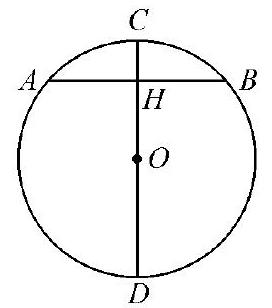
\includegraphics[max width=\textwidth, center]{2024_10_30_66b8e5e701da2093c133g-017(2)}

图2-1

距离称为弦心距,这里 $\triangle O A H$ 是一个重要三角形,它联系着半弦长、半径、弦心距之间的数量关系, 是处理这类问题的重要工具, 而且我们利用这个特殊的直角三角形不难发现:

在同圆 (或等圆)中,弦相等 $\Leftrightarrow$ 弦心距相等。\\
在同圆 (或等圆)中,弦越长 $\Leftrightarrow$ 弦心距越短。\\
例1 如图 2-2 所示, $A B$ 与 $C D$ 是 $\odot O$ 的两条互相垂直的弦,它们将圆 $O$ 分成四个部分,若弦 $A B$ 的弦心距为 $a$ ,弦 $C D$ 的弦心距为 $b$ ,求最大与最小两部分之和减去其他两部分之和的差。

分析 考虑到各部分形状,从而不便直接计算各部分面积,可利用圆的对称性合理分割。\\
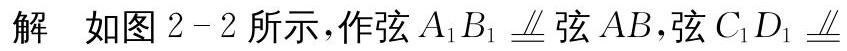
\includegraphics[max width=\textwidth]{2024_10_30_66b8e5e701da2093c133g-017}弦 $C D$ ,则 $\odot O$ 被分割为 9 块,易知四个" $\triangle$ "型全等,四\\
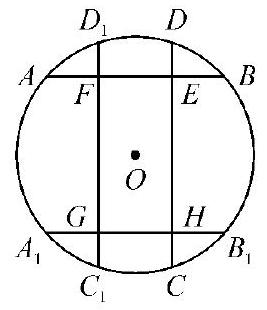
\includegraphics[max width=\textwidth, center]{2024_10_30_66b8e5e701da2093c133g-017(1)}

图2-2\\
" "型中, 上、下两个全等, 左、右两个全等, 从而所求面积恰好等于中间的矩形 $E F G H$ 的面积. 依题意不难得到 $E F=2 b, F G=2 a$ ,所以最大与最小部

分之和与其他两部分之和的差为 $4 a b$ 。\\
说明 本题是巧用圆的对称性的很好范例。\\
例2 如图 2-3 所示,在 $\odot O$ 的直径 $P Q$ 上取一点 $M$ ,过 $M$ 作两条弦 $A B 、 C D$ ,若 $\angle P M A=\angle P M C$ ,求证: $M D=M B$.

分析 可考虑过点 $O$ 作弦 $A B 、 C D$ 的垂线,既是处理这类问题的常见思路,又能集中 $\angle P M A=\angle P M C$ 这一条件于 $\triangle O H M$ 与 $\triangle O G M$ 中.

解 作 $O G \perp C D$ 于点 $G, O H \perp A B$ 于点 $H$, 则在 $\triangle O G M$ 与 $\triangle O H M$ 中,\\
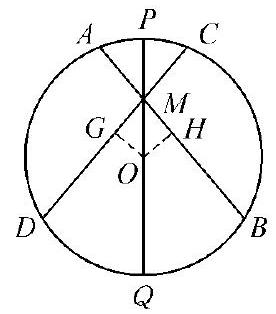
\includegraphics[max width=\textwidth, center]{2024_10_30_66b8e5e701da2093c133g-018}

图2-3\\
$\angle O G M=\angle O H M, \angle O M G=\angle P M C=\angle P M A=\angle O M H$, $O M=O M$ ,从而 $\triangle O G M \cong \triangle O H M$ ,故 $G M=H M, O G=O H$ ,于是 $G D=$ HB.

所以 $M D=M G+G D=M H+H B=M B$.\\
例3 如图 2-4 所示, $\odot O$ 的直径 $A B$ 为 $20 \mathrm{~cm}, G$是直径 $A B$ 上一点, $C D$ 是过 $G$ 的一条弦, $C D=16 \mathrm{~cm}$,过 $A 、 B$ 分别作 $A E \perp C D$ 于点 $E, B F \perp C D$ 于点 $F$,求 $A E$ 与 $B F$ 的长度之差。

分析 作 $O N \perp C D$ 于点 $N$ ,连结 $C O$ ,首先,通过 Rt $\triangle C O N$ 可联系 $A B 、 C D$ 之长;其次,可利用 $\triangle G O N ,$ $\triangle G A E, \triangle G B F$ 之间相似找到 $A E 、 B F$ 的数量关系。\\
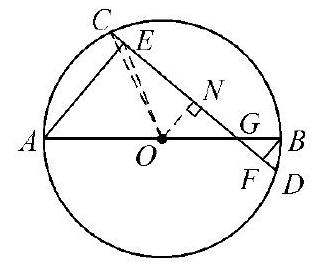
\includegraphics[max width=\textwidth, center]{2024_10_30_66b8e5e701da2093c133g-018(1)}

图2-4

解 作 $O N \perp C D$ 于点 $N$, 连结 $O C$, 则\\
$O N=\sqrt{O C^{2}-C N^{2}}=\sqrt{\left(\frac{1}{2} A B\right)^{2}-\left(\frac{1}{2} C D\right)^{2}}=6(\mathrm{~cm})$,\\
易知

\begin{align*}
\triangle G O N \backsim \triangle G A E \backsim \triangle G B F,
\end{align*}

所以 $\frac{O N}{A E}=\frac{O G}{G A}, \frac{O N}{B F}=\frac{O G}{B G}$, 从而

\begin{align*}
\begin{aligned}
A E-B F & =\frac{O N}{O G} \cdot G A-\frac{O N}{O G} \cdot B G \\
& =\frac{O N}{O G}[O A+O G-(O B-O G)] \\
& =\frac{O N}{O G} \times 2 O G=2 O N=12(\mathrm{~cm})
\end{aligned}
\end{align*}

例 4 如图 2-5 所示, $E F$ 是 $\odot O$ 的直径, $B 、 C$ 在直径 $E F$ 上且 $E B=$\\
$B C=C F$, 点 $A$ 在 $\odot O$ 上. 求证: $A B+A C \leqslant \frac{\sqrt{10}}{3} E F$.\\
分析 注意到点 $O$ 是 $B C$ 的中点及圆的中心对称性, 延长 $A O$ 交 $\odot O$ 于点 $D$, 则四边形 $A B D C$ 为平行四边形, 可建立 $A B 、 A C$ 及直径的数量关系.

解 延长 $A O$ 交 $\odot O$ 于点 $D$ ,连结 $B D 、 C D$ ,又易知 $O$ 为 $B C$ 中点, 所以四边形 $A B D C$ 为平行四边形,\\
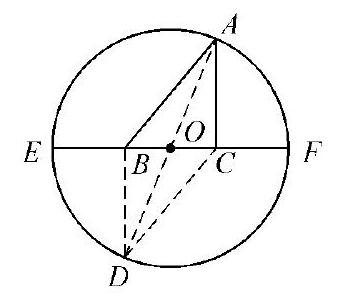
\includegraphics[max width=\textwidth, center]{2024_10_30_66b8e5e701da2093c133g-019}

图2-5

从而

\begin{align*}
2\left(A B^{2}+A C^{2}\right)=A D^{2}+B C^{2}=E F^{2}+\left(\frac{1}{3} E F\right)^{2}=\frac{10}{9} E F^{2}
\end{align*}

又

\begin{align*}
\begin{aligned}
& 2\left(A B^{2}+A C^{2}\right)-(A B+A C)^{2} \\
= & (A B-A C)^{2} \geqslant 0
\end{aligned}
\end{align*}

所以

\begin{align*}
\frac{10}{9} E F^{2}=2\left(A B^{2}+A C^{2}\right) \geqslant(A B+A C)^{2}
\end{align*}

即

\begin{align*}
A B+A C \leqslant \frac{\sqrt{10}}{3} E F
\end{align*}

说明 本题解法中, 延长 $A O$, 实现直径与 $A B 、 A C$ 统一于一个平行四边形之中,是圆的中心对称性的体现。

例5 如图 2-6 所示,已知 $\odot O_{1}$ 与 $\odot O_{2}$ 交于 $P 、 Q$ 两点,过点 $P$ 作割线 $A P B$ 交 $\odot O_{1}$ 于点 $A$, 交 $\odot O_{2}$ 于点 $B$, 且 $A B / / O_{1} O_{2}$; 过点 $P$ 另作割线 $C P D$ 交 $\odot O_{1}$ 于点 $C$, 交 $\odot O_{2}$ 于点 $D$. 请比较 $A B$ 与 $C D$ 的大小.

分析 作 $O_{1} E \perp A B$ 于 $E, O_{2} F \perp A B$ 于\\
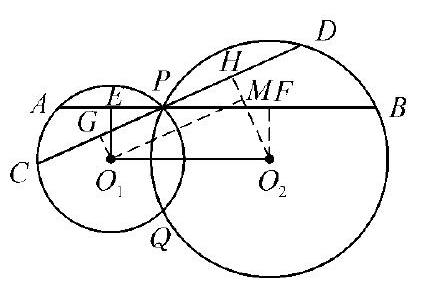
\includegraphics[max width=\textwidth, center]{2024_10_30_66b8e5e701da2093c133g-019(1)}

图2-6\\
$F$, 则 $O_{1} O_{2}=\frac{1}{2} A B$, 实现 $A B$ 长度与 $O_{1} O_{2}$ 长度的转化. 同样地, 作 $O_{1} G \perp$ $C D$ 于 $G, O_{2} H \perp C D$ 于 $H$, 再作 $O_{1} M \perp O_{2} H$ 于 $M$, 则 $O_{1} M=\frac{1}{2} C D$. 从而将 $A B 、 C D$ 的长度统一于 Rt $\triangle M O_{1} O_{2}$ 中, 问题可解.

解 作 $O_{1} E \perp A B$ 于 $E, O_{2} F \perp A B$ 于 $F$, 则 $O_{1} O_{2}=\frac{1}{2} A B$, 作 $O_{1} G \perp$ $C D$ 于 $G, O_{2} H \perp C D$ 于 $H$, 作 $O_{1} M \perp O_{2} H$ 于 $M$, 则 $O_{1} M=\frac{1}{2} C D$. 在 Rt $\triangle O_{1} O_{2} M$ 中, $O_{1} M<O_{1} O_{2}$, 所以 $\frac{1}{2} C D<\frac{1}{2} A B$, 即 $C D<A B$.

例6 如图 2-7所示,在 $\odot O$ 中任意作两条半径 $O A$ 、 $O B$, 过点 $A$ 作 $A C \perp O B$ 于点 $C$, 过点 $C$ 作 $C P \perp A B$ 于点 $P$,连结 $O P$ 。求证: $O P^{2}+C P^{2}=R^{2}$ (这里 $R$ 是 $\odot O$ 的半径)。

分析 结论的形式提示应作 $O H \perp A B$ 于点 $H$ ,利用勾股定理。

解 作 $O H \perp A B$ 于点 $H$ ,则

\begin{align*}
\begin{aligned}
O P^{2} & =O H^{2}+H P^{2} \\
& =O B^{2}-H B^{2}+H P^{2} \\
& =R^{2}-\frac{1}{4} A B^{2}+H P^{2}
\end{aligned}
\end{align*}

\begin{center}
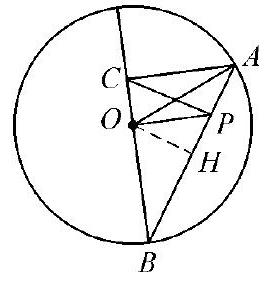
\includegraphics[max width=\textwidth]{2024_10_30_66b8e5e701da2093c133g-020(1)}
\end{center}

图2-7

在 Rt $\triangle A C B$ 中, $C P \perp A B$ 于点 $P$,故 $A C^{2}=A P \cdot A B$ (射影定理), 从而,

\begin{align*}
\begin{align*}
C P^{2} & =A C^{2}-A P^{2} \\
& =A P \cdot A B-A P^{2} \\
& =A P(A B-A P)=A P \cdot P B \\
& =(A H-H P)(H B+H P) \\
& =\frac{1}{4} A B^{2}-H P^{2},
\end{align*} \tag{2}
\end{align*}

(1) +(2)得:

\begin{align*}
O P^{2}+C P^{2}=R^{2}
\end{align*}

说明 $C P^{2}=A P \cdot P B$ 也可由 $\triangle A C P \backsim \triangle C B P$ 直接得到.

\section*{习 题 2}
1 直角三角形中, $\angle C=90^{\circ}, A C=8, C B=15$, 以点 $C$ 为圆心、半径为 8的圆交 $A B$ 于点 $D$, 求 $B D$ 之长.\\
2 如图所示, $A B$ 为 $\odot O$ 的弦,点 $G 、 H$ 都在 $A B$ 上,且 $A G=B H$ ,分别过点 $G 、 H$ 作弦 $C D 、 E F$ ,若 $\angle D G B=\angle F H A$ ,求证: $C D=E F$ 。\\
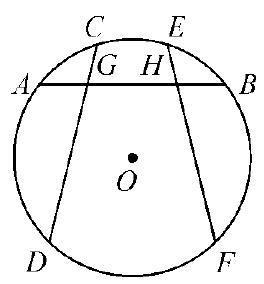
\includegraphics[max width=\textwidth, center]{2024_10_30_66b8e5e701da2093c133g-020}\\
(第2题)\\
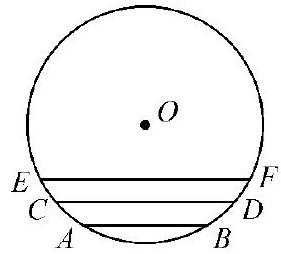
\includegraphics[max width=\textwidth, center]{2024_10_30_66b8e5e701da2093c133g-020(2)}\\
(第3题)

3 如图, $A B 、 C D 、 E F$ 是 $\odot O$ 的三条互相平行的弦,且 $E F$ 与 $C D$ 之间的距离等于 $C D$ 与 $A B$ 之间的距离。若 $A B=6, C D=8, E F=2 \sqrt{21}$, 求 $\odot O$ 的半径。\\
4 已知 $A B$ 为 $\odot O$ 的直径, $P$ 为 $A B$ 上一点, 过点 $P$ 作弦 $C D$, 若 $\angle D P B=$ $45^{\circ}$ ,求证: $P C^{2}+P D^{2}=2 O A^{2}$ 。\\
5 如图, $C$ 为 $\odot O$ 上一点, $A B$ 为直径,作 $O D \perp A C$ 于 $D$ ,连结 $B D$ 交 $O C$ 于点 $G$, 若 $B D=9$, 求 $D G$ 之长。\\
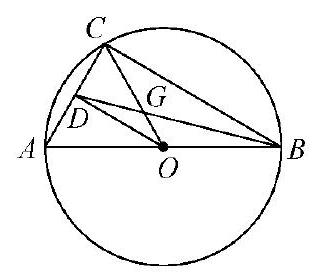
\includegraphics[max width=\textwidth, center]{2024_10_30_66b8e5e701da2093c133g-021(2)}\\
(第 $\mathbf{5}$ 题)\\
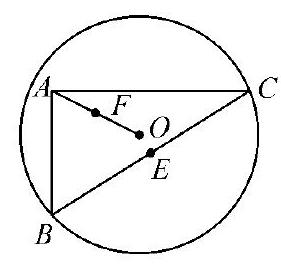
\includegraphics[max width=\textwidth, center]{2024_10_30_66b8e5e701da2093c133g-021}\\
(第 6 题)

6 如图, $A$ 是半径为 $R$ 的 $\odot O$ 内一定点, $O A=m$, 过点 $A$ 作 $A C$ 交 $\odot O$ 于点 $C, A B$ 交 $\odot O$ 于点 $B$ 且 $\angle B A C=90^{\circ}$, 已知 $E$ 为 $B C$ 中点, $F$ 为 $A O$ 中点,求 $E F$ 。\\
7 如图,半径给定的两圆同心,对小圆作三条切线,两两分别交于 $A 、 B 、 C$三点, 记以 $A 、 B 、 C$ 为顶点的像扇形的区域面积分别为 $S_{1} 、 S_{2} 、 S_{3}$, $\triangle A B C$ 的面积为 $S$ 。求证: $S_{1}+S_{2}+S_{3}-S$ 为定值。\\
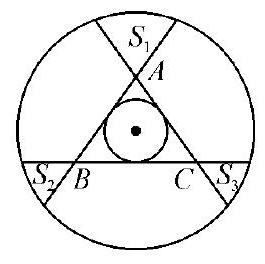
\includegraphics[max width=\textwidth, center]{2024_10_30_66b8e5e701da2093c133g-021(1)}\\
(第 7 题)\\
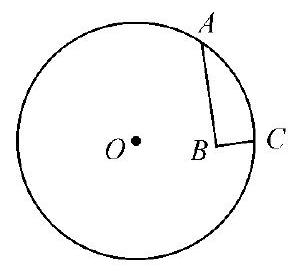
\includegraphics[max width=\textwidth, center]{2024_10_30_66b8e5e701da2093c133g-021(3)}\\
(第 8 题)

8 如图, $\odot O$ 中有两点 $A 、 C, B$ 在 $\odot O$ 内,若 $A B=6, B C=2, A B \perp B C$, $\odot O$ 的半径为 $5 \sqrt{2}$, 求 $O B$.

\section*{与圆有关的角}
圆的半径、直径、弦、割线、切线相交都会形成角,圆的许多问题都涉及到这些与圆有关的角,本节我们来谈谈这些角。

圆外角:顶点在圆外,两边和圆相交(或相切)的角称为圆外角。\\
弦切角:顶点在圆上,一条边和圆相交,另一边和圆相切的角称为弦切角。\\
圆周角:顶点在圆上,两条边都和圆相交的角称为圆周角。\\
圆内角:顶点在圆内,两边和圆相交的角称为圆内角。特别地,顶点在圆心的圆内角又称作圆心角。

关于这些角我们有如下结论:\\
(1)圆心角的度数等于它所对弧的度数;\\
(2)圆周角的度数等于它所对弧的度数的一半;\\
(3)同弧所对圆心角是圆周角的两倍;\\
(4)同弧或等弧所对圆周角相等;同圆或等圆中,相等的圆周角所对弧也相等;\\
(5)半圆(或直径)所对圆周角为直角;直角所对弦为直径;\\
(6)弦切角等于它所夹弧所对的圆周角。\\
例1 已知 $\triangle A B C$ 的外接圆为 $\odot O, \odot O_{1}$ 经过 $A 、 B 、 O$ 且分别交 $B C 、 A C$ 于 $E 、 D$ (异于 $B 、 A$ 的点), 求证: $C O \perp D E$ 。

证明 因为 $A 、 B 、 E 、 D$ 共于 $\odot O_{1}$, 故 $\angle D E C=$ $\angle B A C$ (四点共圆的性质).

连结 $O B 、 O C$, 则 $\angle B O C=2 \angle B A C=$ $2 \angle D E C$ ,且\\
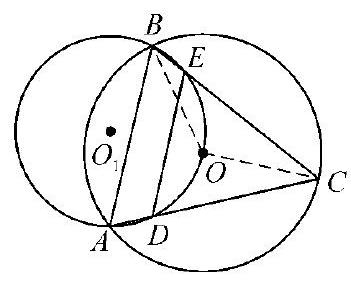
\includegraphics[max width=\textwidth, center]{2024_10_30_66b8e5e701da2093c133g-022}

图3-1

\begin{align*}
\begin{aligned}
\angle O C B & =\frac{180^{\circ}-\angle B O C}{2} \\
& =90^{\circ}-\frac{1}{2} \angle B O C \\
& =90^{\circ}-\angle D E C
\end{aligned}
\end{align*}

即\\
$\angle O C B+\angle D E C=90^{\circ}$ ,故 $C O \perp D E$ 。\\
例2 已知 $I$ 是 $\triangle A B C$ 的内心,连结 $A I$ 交 $\triangle A B C$外接圆于 $D$ ,连结 $B D 、 D C$ ,求证: $B D=D I=D C$ 。

证明 连结 $B I$ ,则

又

\begin{align*}
\begin{aligned}
\angle B I D & =\frac{1}{2} \angle B A C+\frac{1}{2} \angle A B C \\
\angle I B D & =\angle I B C+\angle C B D \\
& =\frac{1}{2} \angle A B C+\angle D A C \\
& =\frac{1}{2} \angle A B C+\frac{1}{2} \angle B A C
\end{aligned}
\end{align*}

\begin{center}
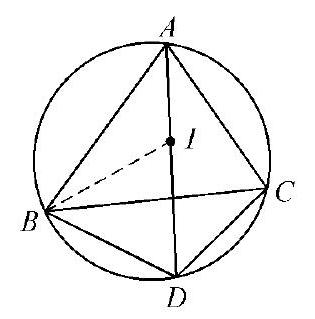
\includegraphics[max width=\textwidth]{2024_10_30_66b8e5e701da2093c133g-023(1)}
\end{center}

图3-2

所以 $\angle B I D=\angle I B D$, 从而 $B D=D I$.\\
又因为 $A I$ 平分 $\angle B A C$, 所以 $\overparen{B D}=\overparen{D C}$, 从而 $B D=D C$, 于是 $B D=$ $D I=D C$.

说明 本例虽易,但它是 $\triangle A B C$ 内心的一个性质。有人戏称为"鸡爪子定理".

例 3 点 $P$ 为正方形 $A B C D$ 外接圆 $O$ 的弧 $\overparen{A D}$ 上一点, 连结 $P A 、 P B$ 、 $P C$, 求 $\frac{P A+P C}{P B}$ 之值.

分析 注意到 $\angle P A D+\angle P C B \stackrel{m}{=} \frac{1}{2} \overparen{D P}+$ $\frac{1}{2} \overparen{P B}=90^{\circ}, \angle D A B=90^{\circ}$ ,且 $B C=B A$ ,可将 $\triangle P B C$ 绕 $B$ 逆时针转 $90^{\circ}$ ,实现 $P A 、 P C$ 共于一线,以便求解。

解 延长 $P A$ 与过点 $B$ 垂直于 $P B$ 的直线\\
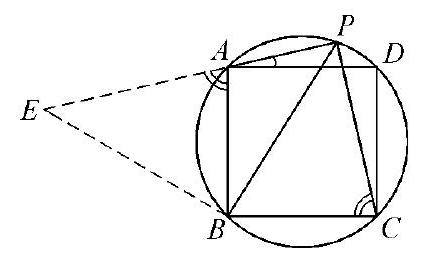
\includegraphics[max width=\textwidth, center]{2024_10_30_66b8e5e701da2093c133g-023}

图3-3

交于点 $E$ 。

由 $A 、 B 、 C 、 P$ 共圆, 可得 $\angle E A B=\angle P C B$.\\
由于 $\angle E B A 、 \angle P B C$ 均为 $\angle A B P$ 的余角, 故 $\angle E B A=\angle P B C$, 结合 $A B=C B$ ,我们可得到 $\triangle E A B \cong \triangle P C B$ ,所以 $E B=P B, E A=P C$ 。由于 $\triangle E B P$ 为等腰直角三角形, 于是 $\frac{P A+P C}{P B}=\frac{P A+A E}{P B}=\frac{E P}{P B}=$ $\sqrt{2}$.

例 $4 \odot O$ 是六边形 $A G B H C K$ 的外接圆, $\odot I$ 内切于 $\triangle A B C$, 点 $D 、 E 、 F$ 为切点 (如图), 若 $\angle D E F=55^{\circ}$, $\angle D F E=60^{\circ}$, 求 $\angle G 、 \angle H 、 \angle K$ 。

分析 由于 $A B 、 A C$ 切 $\odot I$ ,故 $\angle A F E=\angle A E F=$ $\angle F D E=180^{\circ}-\angle D E F-\angle D F E=65^{\circ}$ ,从而 $\angle B A C$ 可求,又 $\angle B A C+\angle B H C=180^{\circ}$ ,故 $\angle H$ 可求。

解 因为 $A B 、 A C$ 切 $\odot I$ 于点 $F 、 E$ ,故 $\angle A F E=$\\
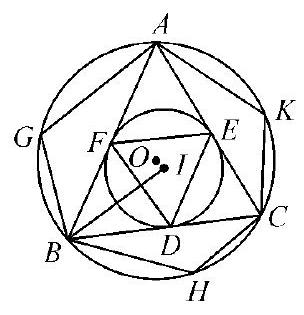
\includegraphics[max width=\textwidth, center]{2024_10_30_66b8e5e701da2093c133g-024}

图3-4\\
$\angle A E F=\angle E D F$.

因为 $\angle F D E=180^{\circ}-\angle D E F-\angle D F E=180^{\circ}-55^{\circ}-60^{\circ}=65^{\circ}$,\\
所以

\begin{align*}
\angle A F E=\angle A E F=65^{\circ},
\end{align*}

从而

\begin{align*}
\angle B A C=180^{\circ}-\angle A F E-\angle A E F=50^{\circ} .
\end{align*}

由于

\begin{align*}
\angle B A C+\angle B H C \stackrel{m}{=} \frac{1}{2} \overparen{B A C}+\frac{1}{2} \widehat{B H C}=180^{\circ}
\end{align*}

所以 $\angle B H C=130^{\circ}$.\\
同理 $\angle A G B=120^{\circ}, \angle A K C=110^{\circ}$ 。\\
即 $\angle G 、 \angle H 、 \angle K$ 分别为 $120^{\circ} 、 130^{\circ} 、 110^{\circ}$ 。\\
例 5 如图 3-5, 四边形 $A B C D$ 内接于圆 $O$ ,对角线 $A C 、 B D$ 交于点 $F$, 延长 $B A 、 C D$ 交于点 $P, P K$ 平分 $\angle B P C$ ,过点 $F$ 作 $E F \perp P K$ 于点 $E$ ,交 $P B 、 P C$ 于点 $M$ 、 $N$ ,求证: $\angle A F M=\angle B F M$ 。

分析 虽然图形稍显复杂,但仔细分析与之相关的角的关系,不难得到证明。

证明 $M N$ 垂直于 $\angle B P C$ 的角平分线,易证 $\triangle P M E \cong$ $\triangle P N E$ ,所以 $\angle P M N=\angle P N M$ 。

又 $\angle P M N=\angle A B D+\angle B F M$,\\
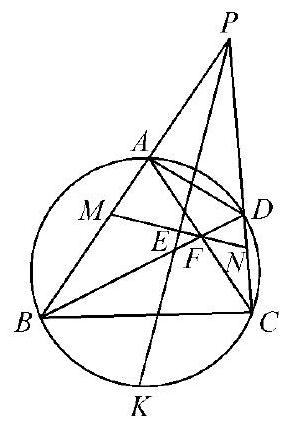
\includegraphics[max width=\textwidth, center]{2024_10_30_66b8e5e701da2093c133g-024(1)}

图3-5\\
$\angle P N M=\angle D C A+\angle C F N$,

注意到\\
所以\\
又\\
所以

\begin{align*}
\angle A B D=\angle D C A,
\end{align*}

$\angle B F M=\angle C F N$.\\
$\angle C F N=\angle A F M$,\\
$\angle B F M=\angle A F M$.

例 6 在凸四边形 $A B C D$ 中, $\angle B A C=20^{\circ}, \angle B C A=30^{\circ}, \angle B D C=$ $40^{\circ}, \angle B D A=60^{\circ}$, 若对角线 $A C 、 B D$ 交于点 $P$, 求 $\angle C P B$.

分析 由 $\angle B A C=\frac{1}{2} \angle B D C, \angle B C A=\frac{1}{2} \angle B D A$ 联想到圆的圆心角与圆周角的关系,从而考虑作 $\triangle A B C$ 的外接圆。

解 作 $\triangle A B C$ 的外接圆,延长 $B D$ 交 $\triangle A B C$ 外接圆于点 $E$, 连结 $A E 、 E C$, 则 $\angle A E B=\angle A C B=30^{\circ}, \angle C E B=$ $\angle B A C=20^{\circ}$ 。

又 $\angle B D A=60^{\circ}$ ,所以 $\angle E A D=\angle B D A-\angle A E B=$ $30^{\circ}$ ,从而 $D A=D E$ 。同理 $D E=D C$ ,即 $D A=D E=D C ,$所以 $D$ 为外接圆圆心,从而\\
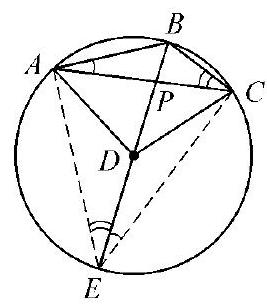
\includegraphics[max width=\textwidth, center]{2024_10_30_66b8e5e701da2093c133g-025(1)}

图3-6

\begin{align*}
\begin{gathered}
\angle A D C=2 \angle A E C=100^{\circ}, \\
\angle D A C=\angle D C A=\frac{180^{\circ}-\angle A D C}{2}=\frac{180^{\circ}-100^{\circ}}{2}=40^{\circ} .
\end{gathered}
\end{align*}

于是

\begin{align*}
\begin{aligned}
\angle C P B & =\angle B E C+\angle E C A \\
& =\angle B E C+\angle E C D+\angle D C A \\
& =20^{\circ}+20^{\circ}+40^{\circ}=80^{\circ} .
\end{aligned}
\end{align*}

说明 "同弧所对圆周角相等"是圆中等角转换的"转换器".\\
例7 如图, $I$ 是 $\triangle A B C$ 的内心, $I_{1}$ 是 $\triangle A B C$ 的边 $B C$ 一侧的旁心,连结 $I I_{1}$ 交 $\triangle A B C$ 的外接圆于点 $E$ ,求证: $I E=I_{1} E$ 。

证明 因 $I C 、 I_{1} C$ 分别平分 $\angle A C B 、 \angle B C D$ 且 $\angle A C B+\angle B C D=180^{\circ}$, 故 $\angle I C I_{1}=90^{\circ}$ 。易知 $A$ 、 $I 、 I_{1}$ 共线,

又 $\angle C I E=\angle C A E+\angle A C F \stackrel{m}{=} \frac{1}{2}(\overparen{A F}+\overparen{C E})$,\\
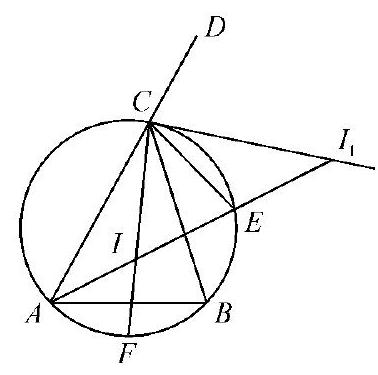
\includegraphics[max width=\textwidth, center]{2024_10_30_66b8e5e701da2093c133g-025}

图3-7

\begin{align*}
\angle I C E \stackrel{m}{=} \frac{1}{2}(\overparen{B F}+\overparen{B E}),
\end{align*}

注意到 $\angle A C F=\angle F C B$ 有 $\overparen{A F}=\overparen{F B}, \angle C A E=\angle E A B$ 有 $\overparen{C E}=\overparen{B E}$ ,从而 $\angle C I E=\angle I C E$ ,即有

\begin{align*}
I E=C E, \tag{1}
\end{align*}

又

\begin{align*}
\angle E C I_{1}=90^{\circ}-\angle E C I=90^{\circ}-\angle C I E=\angle I I_{1} C,
\end{align*}

由(1)(2)知 $I E=I_{1} E$ 。\\
例 8 四边形 $A B C D$ 内接于 $\odot O$, 且对角线 $A C$ 与对角线 $B D$ 垂直, 过点 $O$ 作 $O H \perp A D$ 于 $H$ 。求证: $O H=\frac{1}{2} B C$ 。

证明 连结 $D O$ 并延长交 $\odot O$ 于点 $E$ ,连结 $A E$ ,由于 $D E$ 为直径,故 $A E \perp A D$ ,又 $O H \perp A D$ ,故 $O H / /$ $A E$ ,注意到 $O$ 是 $D E$ 中点,从而

\begin{align*}
O H=\frac{1}{2} A E \tag{1}
\end{align*}

又 $\quad \frac{1}{2}(\overparen{A D}+\overparen{A E}) \stackrel{m}{=} 90^{\circ}$ ,\\
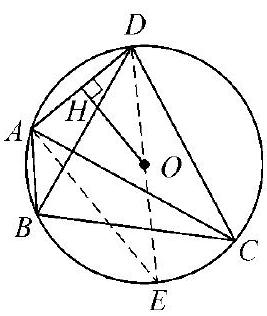
\includegraphics[max width=\textwidth, center]{2024_10_30_66b8e5e701da2093c133g-026}

图3-8

由于 $A C \perp B D$, 故 $\frac{1}{2}(\overparen{A D}+\overparen{B C}) \stackrel{m}{=} 90^{\circ}$.\\
从而 $\overparen{A E}=\overparen{B C}$ ,即有 $A E=B C ,$\\
由(1)、(2)知 $O H=\frac{1}{2} B C$.\\
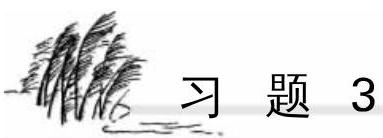
\includegraphics[max width=\textwidth, center]{2024_10_30_66b8e5e701da2093c133g-026(1)}

1 如图, 锐角 $\triangle A B C$ 中, $A D \perp B C$ 于点 $D, A E$ 是 $\triangle A B C$ 外接圆直径, $M$ 是 $\overparen{B C}$ 中点. 求证: $\angle E A M=\angle D A M$.\\
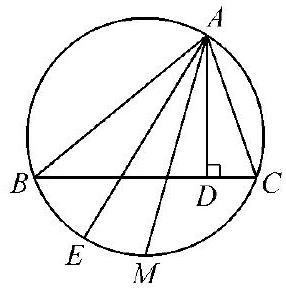
\includegraphics[max width=\textwidth, center]{2024_10_30_66b8e5e701da2093c133g-026(3)}\\
(第 1 题)\\
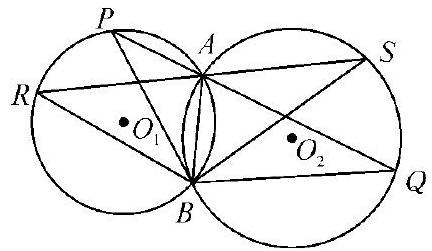
\includegraphics[max width=\textwidth, center]{2024_10_30_66b8e5e701da2093c133g-026(2)}\\
(第2 题)

2 如图,两圆相交于 $A 、 B$ 两点,过 $A$ 作割线 $P Q$ 交 $\odot O_{1}$ 于 $P$ ,交 $\odot O_{2}$ 于 $Q$ ;过 $A$ 作割线 $R S$ 交 $\odot O_{1}$ 于 $R$ ,交 $\odot O_{2}$ 于 $S$ 。求证: $\angle P B R=\angle S B Q$.

3 如图, $\odot O$ 的两条弦 $A B 、 D C$ 的延长线相交于点 $P$ ,且 $\angle P=90^{\circ}$ ,连结 $O A, O B, O C, O D, A D, B C$, 求证: $S_{\triangle O A D}=S_{\triangle O B C}$.\\
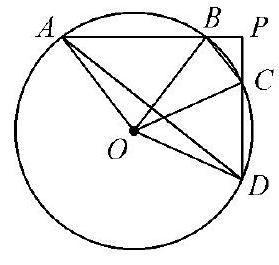
\includegraphics[max width=\textwidth, center]{2024_10_30_66b8e5e701da2093c133g-027(4)}\\
(第3题)\\
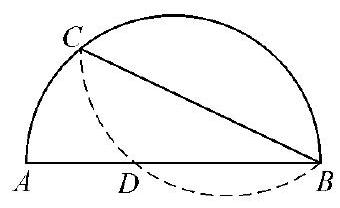
\includegraphics[max width=\textwidth, center]{2024_10_30_66b8e5e701da2093c133g-027(1)}\\
(第4 题)

4 如图, $C$ 是半圆上一点, $A B$ 是直径,将弓形沿 $B C$ 翻折交 $A B$ 于点 $D$ ,若 $A D=4, D B=5$ ,求 $B C$ 之长。\\
5 如图,四边形 $A B D C$ 内接于 $\odot O, E$ 在 $A D$ 上,且 $A B=A E=A C$, 求证:\\
(1) $\angle C A D=2 \angle D B E$;\\
(2) $A D^{2}-A B^{2}=B D \cdot D C$.\\
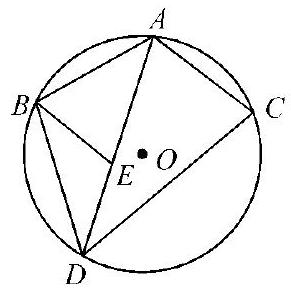
\includegraphics[max width=\textwidth, center]{2024_10_30_66b8e5e701da2093c133g-027}\\
(第 5 题)\\
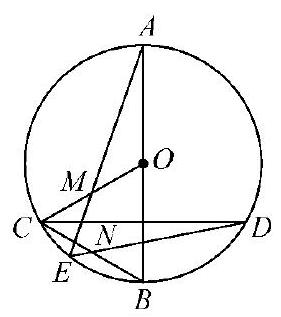
\includegraphics[max width=\textwidth, center]{2024_10_30_66b8e5e701da2093c133g-027(2)}\\
(第 6 题)

6 如图, $\odot O$ 中弦 $C D$ 垂直于直径 $A B, M$ 是 $O C$ 中点, $A M$ 延长线交 $\odot O$ 于点 $E, B C$ 交 $E D$ 于点 $N$. 求证: $B N=C N$.\\
7 如图,五边形 $A B C D E$ 内接于圆,且 $A C / / D E, B D / / A E, C E / / A B$ , $D A / / B C, E B / / C D$ ,求证:五边形 $A B C D$ 为正五边形。\\
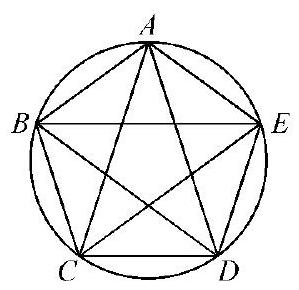
\includegraphics[max width=\textwidth, center]{2024_10_30_66b8e5e701da2093c133g-027(5)}\\
(第7题)\\
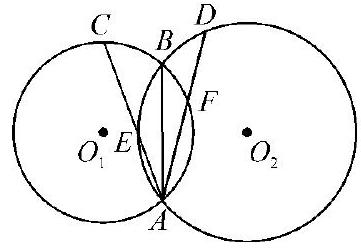
\includegraphics[max width=\textwidth, center]{2024_10_30_66b8e5e701da2093c133g-027(3)}\\
(第8题)

8 如图, $\odot O_{1}$ 与 $\odot O_{2}$ 交于点 $A 、 B, \odot O_{1}$ 的弦 $A C$ 交 $\odot O_{2}$ 于点 $E, \odot O_{2}$ 的弦 $A D$ 交 $\odot O_{1}$ 于点 $F$, 求证: $C E=D F$ 的充要条件是 $A B$ 平分 $\angle C A D$.

9 如图,四边形 $A B C D$ 内接于圆 $O$ ,延长 $A D$ 、 $B C$ 交于点 $F$, 延长 $D C 、 A B$ 交于点 $E$, $\angle A E C$ 的平分线交 $B C$ 于点 $M$, 交 $A D$ 于点 $N, \angle B F D$ 的平分线交 $A B$ 于点 $P$, 交 $C D$于点 $Q$. 求证: 四边形 $M P N Q$ 是菱形.\\
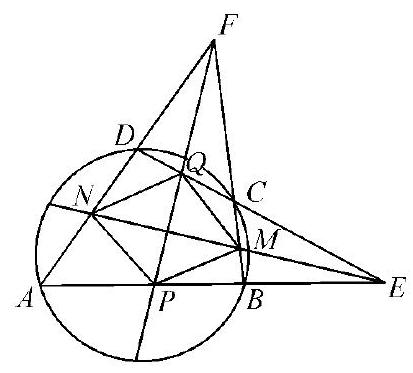
\includegraphics[max width=\textwidth, center]{2024_10_30_66b8e5e701da2093c133g-028}\\
(第9 题)

\section*{与圆相关的位置关系}
我们知道点与圆有三种位置关系: 点在圆外、点在圆上、点在圆内, 通常我用点到圆心的距离 $d$ 与圆的半径 $R$ 来反映这三种关系, 即

点在圆外 $\Leftrightarrow d>R$ ;\\
点在圆上 $\Leftrightarrow d=R$ ;\\
点在圆内 $\Leftrightarrow d<R$.\\
事实上,还有一种方式也可反映点与圆的位置关系,如图 4-1, $A B$ 是 $\odot O$ 的一条弦,点 $Q$ 在弧 $\overparen{A B}$ 上。设 $\angle A Q B=\alpha$, 若点 $P$ 与点 $Q$ 在弦 $A B$ 的同侧, 则

点 $P$ 在圆外 $\Leftrightarrow \angle A P B<\alpha ;$\\
点 $P$ 在圆上 $\Leftrightarrow \angle A P B=\alpha$;\\
点 $P$ 在圆内 $\Leftrightarrow \angle A P B>\alpha$.\\
例1 如图 4-2 所示, $\odot D$ 与 $\odot O$ 相交于点 $A$ 、 $B$, 过点 $B$ 作 $\odot D$ 的切线交 $\odot O$ 于点 $C$, 若 $A B=B C$,判断点 $O$ 与 $\odot D$ 的位置关系.

分析 猜想点 $O$ 在 $\odot D$ 上, 从条件看: $O A=$ $O B=O C, B C$ 是切线, $A B$ 是公共弦, 从角度方面可证 $O D=D B$ 。\\
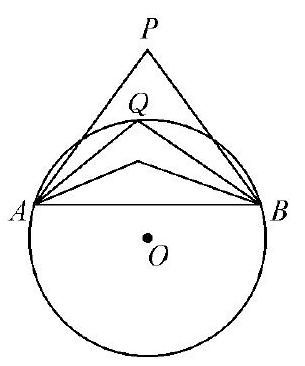
\includegraphics[max width=\textwidth, center]{2024_10_30_66b8e5e701da2093c133g-029(1)}

图4-1\\
\includegraphics[max width=\textwidth, center]{2024_10_30_66b8e5e701da2093c133g-029}

图4-2

解 连结 $O A 、 O B 、 O C$, 在 $\triangle O B C$ 与 $\triangle O B A$ 中, $A B=B C, O A=O C$, $O B$ 为公共边, 从而 $\triangle O B C \cong \triangle O B A$, 故 $\angle O B A=\angle O B C$, 又 $B C$ 为 $\odot D$ 的切线, 所以 $\angle D B C=90^{\circ}, A B$ 为 $\odot D$ 与 $\odot O$ 的公共弦, $O D$ 是两圆连心线, 故 $O D \perp A B$, 于是

\begin{align*}
\angle D B O=90^{\circ}-\angle O B C=90^{\circ}-\angle O B A=\angle D O B,
\end{align*}

即有 $D O=D B$, 这说明点 $O$ 在圆 $D$ 上.\\
例 2 平面上有 $2 n+3$ 个点, 任意三点不共线, 任意四点不共圆, 能否作一圆恰好通过其中三点, 其余 $2 n$ 个点中有 $n$ 点在圆内, 有 $n$ 点在圆外 ?

解 可以. 由于没有三点共线,且仅有有限个点,故一定存在两点,不妨称为点 $A 、 B$, 使得其余各点都在直线 $A B$ 的一侧. 又由于无四点共圆, 故这些点对 $A B$ 的张角互不相等,不妨设 $\angle A P_{1} B<\angle A P_{2} B<\cdots<\angle A P_{n+1} B<\cdots<$ $\angle A P_{2 n+1} B$, 于是过点 $A 、 B 、 P_{n+1}$ 作圆 $O$, 则 $\odot O$ 恰好过点 $A 、 B 、 P_{n+1}$ 三点,点 $P_{1}, P_{2}, \cdots, P_{n}$ 这 $n$ 个点在圆外, $P_{n+2}, \cdots, P_{2 n+1}$ 这 $n$ 个点在圆内.

直线与圆的位置关系有三种:相离、相切、相交. 设圆心到直线的距离为 $d$ ,圆的半径为 $R$ ,则

\begin{align*}
\begin{aligned}
& d>R \Leftrightarrow \text { 相离 } \Leftrightarrow \text { 直线与圆没有公共点, } \\
& d=R \Leftrightarrow \text { 相切 } \Leftrightarrow \text { 直线与圆有唯一公共点, } \\
& d<R \Leftrightarrow \text { 相交 } \Leftrightarrow \text { 直线与圆有两个公共点. }
\end{aligned}
\end{align*}

例 3 已知 Rt $\triangle A B C$ 中, $\angle C=90^{\circ}, A C=3, B C=4$ ,以点 $C$ 为圆心,半径为 $R$ 作 $\odot C$ 。设 $\odot C$ 与线段 $A B$ 的公共点个数为 $n$, 求 $n$ 的所有可能值及相应 $R$ 的取值范围。

分析 "线段 $A B$ "这一条件易疏忽.\\
解 在 Rt $\triangle A B C$ 中, $\angle C=90^{\circ}, A C=3, B C=4$ ,由勾股定理易得 $A B=5$, 又设点 $C$ 到 $A B$ 的距离为 $d$, 则 $\frac{1}{2} A C \cdot B C=\frac{1}{2} A B \cdot d$, 从而 $d=$ 2. 4.\\
(1) $n=0$ ,此时 $0<R<2.4$ 或 $R>4$ ;\\
(2) $n=1$ ,此时 $R=2.4$ 或 $3<R \leqslant 4$ ;\\
(3) $n=2$ ,此时 $2.4<R \leqslant 3$ 。\\
例 4 如图 4-3 所示,等腰梯形 $A B C D$ 中, $C D / / A B, \angle B=60^{\circ}$ ,以 $A D$ 为直径的圆 $O$ 交 $A B$ 于点 $E, \odot O$ 的切线 $E F$ 交 $B C$ 于点 $F$, 若 $D F$也是 $\odot O$ 的切线,求 $C D$ 与 $A B$ 的比值。

分析 可将 $C D 、 A B$ 统一于 $\triangle O E F$ 中寻求其数量关系。\\
\includegraphics[max width=\textwidth, center]{2024_10_30_66b8e5e701da2093c133g-030}

图4-3

解 设 $C D=x, A B=y$ ,若 $F D 、 F E$ 均为 $\odot O$ 的切线,则易知 $F O \perp$ $D E$ ,又 $A D$ 是 $\odot O$ 的直径,故 $\angle A E D=90^{\circ}$ ,即 $D E \perp A B$ 。从而 $A B / /$ OF // CD.

又 $O$ 是 $A D$ 中点, 故 $F$ 是 $B C$ 中点, 从而 $O F=\frac{x+y}{2}$.\\
另外, $A B / / O F, O$ 是 $A D$ 中点, 所以 $\angle E O F=\angle O E A=\angle A=60^{\circ}$.结合 $E F$ 切 $\odot O$ 于点 $E, O E \perp E F$ 知 $2 O E=O F$ 。

不难知道 $\triangle O A E$ 为正三角形, 从而 $O E=A E=\frac{y-x}{2}$, 于是我们有

\begin{align*}
y-x=2 O E=O F=\frac{x+y}{2}
\end{align*}

即有 $y=3 x$, 所以 $\frac{C D}{A B}=\frac{1}{3}$.\\
圆与圆的位置关系有五种:外离、外切、相交、内切、内含. 设两圆圆心距为 $d$ ,两圆半径分别为 $R 、 r(R \neq r)$ ,则

\begin{align*}
\begin{aligned}
& \text { 外离 } \Leftrightarrow d>R+r \Rightarrow \text { 无公共点, } \\
& \text { 外切 } \Leftrightarrow d=R+r \Rightarrow 1 \text { 个公共点, } \\
& \text { 相交 } \Leftrightarrow|R-r|<d<R+r \Leftrightarrow 2 \text { 个公共点, } \\
& \text { 内切 } \Leftrightarrow d=|R-r| \Rightarrow 1 \text { 个公共点, } \\
& \text { 内含 } \Leftrightarrow 0 \leqslant d<|R-r| \Rightarrow \text { 无公共点. }
\end{aligned}
\end{align*}

特别地,两个半径相等且不重合的圆仅有外离、外切、相交三种位置关系。\\
例 5 已知 $\odot A 、 \odot B$ 的半径均为 $1, A B=10$ ,现将 $\odot B$ 固定不动, $\odot A$沿直线 $A B$ 向 $\odot B$ 方向以每秒 2 个单位的速度匀速运动,同时 $\odot A$ 的半径以每秒 1 个单位速度增加,问何时两圆相切?

分析 相切有外切和内切,弄清变化过程中圆心距、半径,即可得解。\\
解 设经过 $t$ 秒钟两圆相切,则 $d=|10-2 t|, r_{B}=1, r_{A}=1+t$ 。\\
于是, 当两圆外切时, $|10-2 t|=2+t$, 解得 $t=\frac{8}{3}$ 或 $t=12$.\\
当两圆内切时, $|10-2 t|=|t|$, 解得 $t=\frac{10}{3}$ 或 $t=10$.\\
经检验,以上各解均符合要求。\\
例6 如图 $4-4, \odot A 、 \odot B 、 \odot C$ 两两外切,且都与直线 $l$ 相切,若 $\odot A 、 \odot B 、 \odot C$ 的半径分别为 $a 、 b 、 c$, 求证: $\frac{1}{\sqrt{a}}+\frac{1}{\sqrt{b}}=\frac{1}{\sqrt{c}}$.

分析 分别连结圆心与直线 $l$ 的切点,连结 $A C 、 B C 、 A B$ ,我们可得到三个直角梯形,在每个直角梯形中(如图)可计算出 $D E 、 E F 、 D F$ ,\\
\includegraphics[max width=\textwidth, center]{2024_10_30_66b8e5e701da2093c133g-031}

图4-4

由 $D F=D E+E F$ 可建立 $a 、 b 、 c$ 的数量关系式。

解 设 $\odot A 、 \odot B 、 \odot C$ 分别切直线 $l$ 于点 $D 、 F 、 E$, 连结 $A D 、 B F 、 C E$及 $A B 、 A C 、 C B$ ,则 $A D \perp l, B F \perp l, A D=a, B F=b, A B=a+b$ ,于是

\begin{align*}
D F=\sqrt{(a+b)^{2}-(a-b)^{2}}=2 \sqrt{a b} .
\end{align*}

同理 $D E=2 \sqrt{a c}, E F=2 \sqrt{b c}$ ,由于 $D F=D E+E F$ ,故

\begin{align*}
2 \sqrt{a b}=2 \sqrt{a c}+2 \sqrt{b c}
\end{align*}

从而

\begin{align*}
\frac{1}{\sqrt{c}}=\frac{1}{\sqrt{a}}+\frac{1}{\sqrt{b}}
\end{align*}

说明 处理两圆关系时,连心线通常起着重要作用,它是两圆组成图形的对称轴,有许多性质可直接凸显出来。

例7 如图 4-5, 两圆内切于点 $P$, 大圆的弦 $A B$切小圆于点 $Q$, 连结 $P A 、 P B$ 分别交小圆于点 $C 、 D$,连结 $P Q$ 与 $C D$ 交于点 $H$.

求证:(1) $\frac{C H}{A Q}=\frac{H D}{Q B}$ ;\\
(2) $\angle A P Q=\angle Q P B$.

分析 从结论看,应证 $A B / / C D$ ,即证 $\angle A B P=$\\
\includegraphics[max width=\textwidth, center]{2024_10_30_66b8e5e701da2093c133g-032}

图4-5\\
$\angle C D P$, 又注意到两圆内切, 可过点 $P$ 作两圆的公切线 $E F$ ,从而 $\angle A B P=\angle C D P=\angle A P E$ 。

证明 (1) 过点 $P$ 作两圆公切线 $E F$ ,则在小圆中 $\angle C D P=\angle C P E$ ,在大圆中 $\angle A B D=\angle A P E$ ,从而 $\angle C D P=\angle A B P$ ,所以 $A B / / C D$ ,故

\begin{align*}
\frac{C H}{A Q}=\frac{P H}{P Q}=\frac{H D}{Q B} .
\end{align*}

(2)连结 $Q C$ ,则 $\angle A P Q=\angle A Q C, \angle Q P B=\angle Q C H$.\\
由(1)中证明知 $A B / / C D$ ,故 $\angle A Q C=\angle Q C H$ ,从而 $\angle A P Q=\angle Q P B$ 。\\
说明 两圆相切时,过切点作两圆公切线是常见的添加辅助线方法之一,请读者留意。

\section*{习 题 4}
1 平面上有 $2 n+1$ 个点, 能否作一个圆, 使得这 $2 n+1$ 个点中 $n$ 个点在圆内, $n$ 个点在圆外,恰有一点在圆上?\\
2 半径为 2 的圆内能否放进 8 个不重叠的边长为 1 的正方形?

3 已知梯形 $A B C D$ 中, $A D / / B C, A D=1, A B=4, B C=3$,以 $C D$ 中点 $O$ 为圆心,半径为 2 画圆。\\
(1)若 $\odot O$ 与腰 $A B$ 有两个公共点,求 $\angle A B C$ 的取值范围;\\
(2)若 $\odot O$ 与腰 $A B$ 有一个公共点,求 $\angle A B C$ 的取值范围。\\
4 已知 $\odot A 、 \odot B$ 的圆心都在直线 $l$ 上, $A B=3$ ,半径均为 1 ,现 $\odot A$ 以每秒 2 个单位速度沿直线 $l$ 向 $\odot B$ 匀速运动, $\odot B$ 固定不动,同时 $\odot A$ 的半径以每秒 2 个单位的速度增大。\\
(1) $t$ 为何值时,两圆相切?\\
(2) $t$ 为何值时,两圆相交?\\
(3) $t$ 为何值时,两圆相离?\\
5 已知 $\odot O_{1}$ 与 $\odot O_{2}$ 外切,半径分别为 14 和 $7, \odot O_{3}$ 与 $\odot O_{1} 、 \odot O_{2}$ 都内切,且圆心 $O_{3}$ 与圆心 $O_{1}$ 、圆心 $O_{2}$ 共线,又 $\odot O_{4}$ 分别与 $\odot O_{1} 、 \odot O_{2}$ 外切,与 $\odot O_{3}$ 内切,求 $\odot O_{4}$ 的半径。\\
\includegraphics[max width=\textwidth, center]{2024_10_30_66b8e5e701da2093c133g-033}\\
(第 $\mathbf{5}$ 题)

6 长方形 $A B C D$ 中, $A B=1, A D=\sqrt{3}$, 以点 $B$ 为圆心, $B A$ 长为半径作圆交 $B C$ 于点 $E$, 在 $\overparen{A E}$ 上找一点 $P$, 过 $P$ 作 $\odot B$ 的切线交 $A D$ 于点 $S$, 交 $B C$于点 $T$, 若 $S T$ 平分矩形 $A B C D$ 的面积, 求 $S T$ 之长。\\
7 已知点 $D 、 E$ 是 $\triangle A B C$ 的边 $B C$ 上的两点,点 $F$ 在 $B A$ 延长线上, 若 $\angle D A E=\angle C A F$,求证: $\triangle A B D$ 与 $\triangle A E C$ 的外接圆外切。\\
8 在边长为 $a$ 的正方形内放置 5 个半径为 1 的圆,使得任意两圆及圆与正方形的边至多有一个公共点, 求 $a$ 的最小值。\\
\includegraphics[max width=\textwidth, center]{2024_10_30_66b8e5e701da2093c133g-033(1)}\\
(第7题)

当直线与圆有唯一公共点时, 称直线与圆相切, 此唯一公共点称为切点.判定直线与圆相切常用到以下结论:\\
(1) 定义;\\
(2) 圆心到直线的距离等于圆的半径;\\
(3) 经过半径的外端且垂直于半径的直线是圆的切线;\\
(4) 如图 5-1, 点 $A 、 B 、 D$ 在 $\odot O$ 上, 点 $C$ 在 $\odot O$ 外, 若 $\angle B A C=\angle A D B$,则 $A C$ 是 $\odot O$ 的切线 (连结 $A O$ 延长交 $\odot O$ 于另一点 $E$, 连结 $B E$, 即可证明);\\
\includegraphics[max width=\textwidth, center]{2024_10_30_66b8e5e701da2093c133g-034(1)}

图5-1\\
\includegraphics[max width=\textwidth, center]{2024_10_30_66b8e5e701da2093c133g-034}

图5-2\\
(5)如图5-2, 点 $P$ 在圆外, 点 $C$ 在圆上, $P A B$ 是 $\odot O$ 的割线, 若 $P C^{2}=$ $P A \cdot P B$ ,则 $P C$ 是 $\odot O$ 的切线(连结 $A C 、 B C$ ,则 $\triangle P A C \backsim \triangle P C B$ ,即可证明)。

过圆上一点有且仅有一条直线与圆相切,过圆外一点有且仅有两条直线与圆相切.

如图5-3,若 $P$ 是圆外一点, $P E 、 P F$ 分别切 $\odot O$ 于点 $E 、 F$, 若称点 $P$ 到切点的距离为切线长,则用勾股定理易证: $P E=P F$ ,即切线长相等。

运用切线长定理我们不难得到以下熟知的结论:\\
(1)如图5-4, $\triangle A B C$ 外切 $\odot O$ 于点 $D 、 E$ 、 $F$, 设 $A B=c, B C=a, C A=b$, 内切圆半径为 $r$,\\
\includegraphics[max width=\textwidth, center]{2024_10_30_66b8e5e701da2093c133g-034(2)}

图5-3\\
\includegraphics[max width=\textwidth, center]{2024_10_30_66b8e5e701da2093c133g-035(3)}

图5-4\\
\includegraphics[max width=\textwidth, center]{2024_10_30_66b8e5e701da2093c133g-035}

图5-5\\
\includegraphics[max width=\textwidth, center]{2024_10_30_66b8e5e701da2093c133g-035(4)}

图5-6

则 $A E=A F=\frac{b+c-a}{2}, B D=B F=\frac{c+a-b}{2}, C D=C E=\frac{a+b-c}{2}$ ;\\
(2) 如图 $5-5, \mathrm{Rt} \triangle A B C$ 外切 $\odot O$, 内切圆半径为 $r, \angle C=90^{\circ}, A B=c$, $A C=b, B C=a$ ,则 $r=\frac{a+b-c}{2}$ ;\\
(3)如图5-6,凸四边形 $A B C D$ 外切 $\odot O$ ,则 $A B+C D=B C+A D$ ,反之,若凸四边形 $A B C D$ 的对边之和相等,则它一定有内切圆。

例1 如图5-7所示, $B L$ 平分 $\angle A B C, P L$ 切 $\triangle B L C$ 的外接圆于点 $L$, 交 $A B$ 于点 $P$, 求证: $A C$ 是 $\triangle B L P$ 外接圆的切线。

分析 若能证 $\angle A L P=\angle A B L$ ,则命题得证。\\
证明 因 $P L$ 切 $\triangle B L C$ 外接圆于点 $L$, 故 $\angle P L B=$ $\angle C$, 又\\
\includegraphics[max width=\textwidth, center]{2024_10_30_66b8e5e701da2093c133g-035(2)}

图5-7

\begin{align*}
\angle A L P+\angle P L B=\angle A L B=\angle L B C+\angle C,
\end{align*}

所以 $\angle A L P=\angle L B C$.\\
由于 $B L$ 平分 $\angle A B C$, 故 $\angle A B L=\angle L B C$, 从而 $\angle A L P=\angle A B L$.\\
于是 $A C$ 切 $\triangle P B L$ 外接圆于点 $L$ 。\\
例2 如图5-8所示, $\triangle A B C$ 中, $A B=$ $A C, \angle C$ 的平分线交边 $A B$ 于点 $P$, 点 $M$ 为 $\triangle A B C$ 的内切圆 $I$ 与 $B C$ 边的切点,作 $M D / /$ $A C$ 交 $\odot I$ 于点 $D$ 。证明: $P D$ 是 $\odot I$ 的切线。

证明 设 $A B$ 切 $\odot I$ 于点 $E, A C$ 切 $\odot I$ 于点 $F$ ,连结 $I E 、 I F 、 I D 、 I M$ ,则 $I E \perp A B, I F \perp$ $A C, I M \perp B C$, 设 $\angle B C A=2 x$, 则 $\angle F I C=$\\
\includegraphics[max width=\textwidth, center]{2024_10_30_66b8e5e701da2093c133g-035(1)}

图5-8\\
$\angle M I C=90^{\circ}-x, \angle A=180^{\circ}-4 x$ ,从而

\begin{align*}
\angle E I F=360^{\circ}-\angle A E I-\angle A F I-\angle A=4 x
\end{align*}

所以

\begin{align*}
\angle P I E=180^{\circ}-\angle E I F-\angle F I C=90^{\circ}-3 x .
\end{align*}

又 $D M / / A C$ ,故

于是

\begin{align*}
\begin{gathered}
\angle D M C=180^{\circ}-\angle A C M=180^{\circ}-2 x, \\
\angle D M I=90^{\circ}-2 x,
\end{gathered}
\end{align*}

\begin{align*}
\angle D I M=180^{\circ}-2 \angle D M I=4 x
\end{align*}

所以

\begin{align*}
\angle D I P=180^{\circ}-\angle D I M-\angle M I C=90^{\circ}-3 x
\end{align*}

从而 $\angle P I E=\angle P I D$.\\
结合 $I E=I D, I P$ 是公共边, 知 $\triangle P I D \cong \triangle P I E$ ,所以 $\angle P D I=$ $\angle P E I=90^{\circ}$ 。

又 $I D$ 是 $\odot I$ 的半径, $D$ 在 $\odot I$ 上,故 $P D$ 是 $\odot I$ 的切线.\\
说明 若作 $P Q$ 切 $\odot I$ 于点 $Q$ 并延长交 $B C$ 于点 $N$ ,可证 $\triangle N Q M \backsim$ $\triangle A B C$ ,进而可证 $M Q / / A C$ ,结合 $M D / / A C$ ,可知 $Q$ 与 $D$ 重合,从而 $P D$ 是 $\odot I$ 的切线。

例 3 如图 5-9 所示, $\triangle A B C$ 的内切圆分别切 $B C 、 C A 、 A B$ 于点 $D 、 E 、 F, D G \perp E F$ 于 $G$, 求证: $D G$ 平分 $\angle B G C$.

分析 注意到 $\angle A F E=\angle A E F$ ,作 $B M \perp$ $E F$ 于点 $M, C N \perp E F$ 于点 $N$, 则 $\triangle B M F \backsim$ $\triangle C N E$ ,同时由于 $B M / / D G / / C N$ ,造成 $\frac{M G}{N G}$ 向 $\frac{B F}{C E}$ 的有效转化.\\
\includegraphics[max width=\textwidth, center]{2024_10_30_66b8e5e701da2093c133g-036}

图5-9

证明 作 $B M \perp E F$ 于点 $M, C N \perp E F$ 于点 $N$, 由于 $A F 、 A E$ 为 $\triangle A B C$内切圆切线,故 $A F=A E$ 。

从而 $\angle A F E=\angle A E F$ ,于是 $\angle B F M=\angle C E N$ ,结合 $\angle B M F=\angle C N E$,知 $\triangle B M F \backsim \triangle C N E$ ,从而

\begin{align*}
\frac{B M}{C N}=\frac{B F}{C E} \tag{1}
\end{align*}

又 $B M 、 D G 、 C N$ 都垂直于 $E F$, 故 $B M / / D G / / C N$, 所以 $\frac{M G}{N G}=\frac{B D}{D C}$.\\
注意到 $B F 、 B D 、 C D 、 C E$ 均为 $\triangle A B C$ 内切圆的切线. 于是 $B F=B D$, $C D=C E$ ,从而

\begin{align*}
\frac{M G}{N G}=\frac{B F}{C E} \tag{2}
\end{align*}

由(1)、(2)知 $\frac{B M}{C N}=\frac{M G}{N G}$, 又由于 $\triangle B M G 、 \triangle C N G$ 均为直角三角形, 所以 $\triangle B M G \backsim \triangle C N G$ ,从而 $\angle B G M=\angle C G N$ ,故

\begin{align*}
\angle B G D=90^{\circ}-\angle B G M=90^{\circ}-\angle C G N=\angle C G D,
\end{align*}

即 $D G$ 平分 $\angle B G C$ 。\\
说明 若结论成立, 则 $\triangle B F G \backsim \triangle C E G$, 于是希望能证 $\frac{B F}{F G}=\frac{C E}{E G}$, 连结 $D F 、 D E$, 易知 $\angle B F D=\angle D E G$, 为此作 $B P \perp D F$ 于点 $P$, 则 $\triangle B F P \backsim$ $\triangle D E G$. 同理作 $C Q \perp D E$ 于点 $Q$, 则 $\triangle C E Q \backsim \triangle D F G$, 于是此题亦可得证.请读者试试。

例4 如图 5-10所示,三角形 $A B C$的中线 $A D$ 与它的内切圆 $O$ 相交于点 $X$ 、 $Y$ ,若 $A C=A B+A D$ ,求 $\angle X O Y$ 。

分析 设 $O H \perp X Y$ 于点 $H$ ,知道 $O H$与半径 $O X$ 的数量关系,问题即可得解。由\\
\includegraphics[max width=\textwidth, center]{2024_10_30_66b8e5e701da2093c133g-037}

图5-10

于 $\odot O$ 内切于 $\triangle A B C$, 可从面积从手。

解 设 $A B=c, B C=a, C A=b$, 则 $A D=b-c$, 又设 $\odot O$ 的半径为 $r$,作 $O H \perp X Y$ 于点 $H$, 则 $S_{\triangle A B C}=\frac{r}{2}(a+b+c)$.

另一方面, $\quad \frac{1}{2} S_{\triangle A B C}=S_{\triangle A B D}$

\begin{align*}
\begin{aligned}
& =\frac{r c}{2}+\frac{r}{2} B D+\frac{O H}{2} \cdot A D \\
& =\frac{r c}{2}+\frac{r a}{4}+\frac{O H}{2}(b-c)
\end{aligned}
\end{align*}

故

\begin{align*}
\frac{r}{4}(a+b+c)=\frac{r c}{2}+\frac{r a}{4}+\frac{O H}{2}(b-c),
\end{align*}

从而

\begin{align*}
\frac{r}{2}(b-c)=O H(b-c)
\end{align*}

由于 $A C=A B+A D>A B$, 即 $b>c$, 故 $b-c \neq 0$, 从而 $O H=\frac{r}{2}$.\\
故 $\angle X O H=60^{\circ}$, 所以 $\angle X O Y=120^{\circ}$.\\
例 5 如图 5-11 所示, $\triangle A B C$ 的内切圆切 $A B$ 于点 $D, A B$ 边的旁切圆切 $A B$ 于点 $G, B C>A C$, 若 $A D=D G=G B$, 求证: $A B=3(B C-A B)$ 且 $2 A C>B C$.

分析 利用切线长定理并仔细理清各线段关系即可得解。

证明 设 $A B=c, B C=a, C A=b$, 设旁切圆切直线 $C A$ 于点 $J$, 切直线 $C B$ 于点 $H$ ,则 $C J=C H$ 。

\begin{align*}
\text { 又 } B H=B G=\frac{1}{3} c, A J=A G=\frac{2}{3} c \text {, }
\end{align*}

\begin{center}
\includegraphics[max width=\textwidth]{2024_10_30_66b8e5e701da2093c133g-038(2)}
\end{center}

图5-11

且 $C J=C H$, 故 $b+\frac{2}{3} c=a+\frac{1}{3} c$, 即 $c=3(a-b), A B=3(B C-A C)$.\\
由于 $a+b>c=3(a-b)$, 从而 $2 b>a$, 即 $2 A C>B C$.\\
例 6 如图 5-12,半圆 $O_{1}$ 与半圆 $O_{2}$ 相离,它们的直径 $A B 、 C D$ 共线, $A E$切 $\odot O_{2}$ 于点 $E, D F$ 切 $\odot O_{1}$ 于点 $F$, $\odot O_{3}$ 内切 $\odot O_{1}$ 于点 $B$, 切 $A E$ 于点 $H$, $\odot O_{4}$ 内切 $\odot O_{2}$ 于点 $C$, 切 $D F$ 于点 $G$.求证: $\odot O_{3}$ 与 $\odot O_{4}$ 的半径相等.\\
\includegraphics[max width=\textwidth, center]{2024_10_30_66b8e5e701da2093c133g-038}

图5-12

分析 连结 $O_{3} H 、 O_{2} E$ ,则 $O_{3} H / / O_{2} E$ ,有利于计算出 $\odot O_{3}$ 的半径。\\
证明 连结 $O_{3} H 、 O_{2} E$ ,设 $B C=x, \odot O_{i}$ 的半径为 $r_{i}, i=1,2,3,4$ 。\\
于是 $A O_{3}=2 r_{1}-r_{3}, A O_{2}=2 r_{1}+x+r_{2}$, 由于 $O_{3} H \perp A E, O_{2} E \perp A E$,故 $O_{3} H / / O_{2} E$ ,从而 $\frac{O_{3} H}{O_{2} E}=\frac{A O_{3}}{A O_{2}}$ ,即 $\frac{r_{3}}{r_{2}}=\frac{2 r_{1}-r_{3}}{2 r_{1}+x+r_{2}}$ ,解得 $r_{3}=$ $\frac{2 r_{1} r_{2}}{2 r_{1}+2 r_{2}+x}$.

同法可计算得 $r_{4}=\frac{2 r_{1} r_{2}}{2 r_{1}+2 r_{2}+x}$ ,从而 $r_{3}=r_{4}$ 。\\
说明 与两圆都相切的直线称为两圆公切线,公切线夹在两切点间的线段长度称为公切线长,遇到这类问题通常连结两圆圆心、圆心与切点,最终将问题转化为直角三角形来处理。

例 7 如图5-13 所示,线段 $A B$ 把一个边长为 $n$ 的正方形分割成两个多边形(点 $A 、 B$ 在正方形边上),每个多边形都有一个内切圆,其中一个内切圆半径为 6 cm ,另一个内切圆半径大于 6 cm 。求正方形边长与 $A B$ 长度的两倍之差。

分析 分类讨论两个多边形的形状及相应内切圆情况。\\
\includegraphics[max width=\textwidth, center]{2024_10_30_66b8e5e701da2093c133g-038(1)}

图5-13

解 (1)若线段 $A B$ 把正方形分为两个三角形,则此两三角形边全等,从而两个内切圆半径相等,不符合题设条件。\\
(2)若两个多边形中有一个为四边形。如图5-13,则 $A B+C D>2 n>$ $A D+B C$ ,从而四边形 $A B C D$ 不存在内切圆,不符合题设条件。\\
(3)若 $A B$ 将正方形分割为一个三角形和一个五边形,则五边形的内切圆必是正方形内切圆,设此内切圆切 $A B$ 于点 $G$, 切 $A 、 B$ 所在的正方形边于点 $E 、 F$ (如图 5-14 所示), 则 $R F=R E=\frac{n}{2}$. 若五边形内切圆半径为 6 cm ,则 $\triangle A B R$ 的内切圆半径 $<$ $A R<R F=6 \mathrm{~cm}$ ,不符合题设条件。

故 $\triangle A B R$ 的内切圆半径为 6 cm , 设此内切圆切\\
\includegraphics[max width=\textwidth, center]{2024_10_30_66b8e5e701da2093c133g-039(1)}

图5-14\\
$R E$ 于点 $P$, 切 $R F$ 于点 $Q$, 切 $A B$ 于点 $H$, 则 $R Q=$ $R P=6 \mathrm{~cm}$ ,于是

\begin{align*}
\begin{aligned}
n-2 A B & =R F+R E-2 A B \\
& =F A+A Q+Q R+R P+P B+B E-2 A B \\
& =A G+A H+B H+B G-2 A B+R P+R Q \\
& =A G+G B+A H+H B-2 A B+12 \\
& =12(\mathrm{~cm}) .
\end{aligned}
\end{align*}

例8 如图 5-15 所示,给定凸多边形 $A_{1} A_{2} \cdots A_{n}$ ,设 $O$ 为凸多边形内一点,且 $\angle O A_{1} A_{n} \leqslant \angle O A_{1} A_{2}, \angle O A_{2} A_{1} \leqslant \angle O A_{2} A_{3}, \cdots, \angle O A_{n-1} A_{n-2} \leqslant$ $\angle O A_{n-1} A_{n}, \angle O A_{n} A_{n-1} \leqslant \angle O A_{n} A_{1}$, 且这些角均为锐角. 求证: $O$ 是这个凸多边形内切圆圆心.

证明 过点 $O$ 作 $A_{m-1} A_{m}, A_{m} A_{m+1}$ 的垂线,垂足分别为点 $H_{m-1}, H_{m}$ (如图5-15所示),注意到 $\angle O A_{m} A_{m-1} \leqslant \angle O A_{m} A_{m+1}$ ,且均为锐角,所以

\begin{align*}
\begin{aligned}
O H_{m-1} & =O A_{m} \sin \angle O A_{m} A_{m-1} \\
& \leqslant O A_{m} \sin \angle O A_{m} A_{m+1}=O H_{m}
\end{aligned}
\end{align*}

因此有 $O H_{1} \leqslant O H_{2} \leqslant \cdots \leqslant O H_{n} \leqslant O H_{1}$,\\
\includegraphics[max width=\textwidth, center]{2024_10_30_66b8e5e701da2093c133g-039}

图5-15

从而

\begin{align*}
O H_{1}=O H_{2}=\cdots=O H_{n}
\end{align*}

所以凸多边形 $A_{1} A_{2} \cdots A_{n}$ 有内切圆,圆心为 $O$ ,半径为 $O H_{1}$ 。\\
例9 凸四边形 $A B C D$ 中 $A B+C D=B C+A D$ ,求证: $\triangle A B C$ 的内切圆与 $\triangle A C D$ 的内切圆相切。

分析 利用切线长定理证两圆与 $A C$ 切于同一点。

证明 如图 5-16, 设 $\triangle A C D$ 与其内切圆切于点 $E 、 F 、 P, \triangle A B C$ 与其内切圆切于点 $G 、 H$ 、 $Q$, 其中 $P 、 Q$ 都在 $A C$ 上, 则 $A E=A P, A G=$ $A Q, C Q=C H, C F=C P$ 。\\
\includegraphics[max width=\textwidth, center]{2024_10_30_66b8e5e701da2093c133g-040}

图5-16

所以,一方面

\begin{align*}
\begin{aligned}
P Q & =A Q-A P=A G-A E \\
& =(A B-G B)-(A D-D E) \\
& =A B-A D-G B+D E \\
& =A B-A D-B H+D F \\
& =A B-A D-(B C-C H)+(C D-C F) \\
& =A B-A D-B C+C D+C H-C F \\
& =A B+C D-B C-A D+C Q-C P \\
& =A B+C D-(B C+A D)-P Q
\end{aligned}
\end{align*}

即

\begin{align*}
2 P Q=A B+C D-(B C+A D) .
\end{align*}

又 $A B+C D=B C+A D$ ,从而 $P Q=0$ ,即 $P 、 Q$ 重合。\\
故两圆相切, $A C$ 是两圆公切线。\\
例 10 如图5-17, $A B$ 是半圆 $O$ 的直径, $P$ 为直径 $A B$ 上一点,以 $A$ 为圆心 $A P$ 为半径画圆交半圆 $O$ 于点 $C$ ,以 $B$ 为圆心, $B P$ 为半径画圆交半圆 $O$ 于点 $D, M$ 是 $C D$ 中点。

求证: $M P$ 是 $\odot A$ 与 $\odot B$ 的公切线.\\
证明 连结 $A C 、 B D 、 A D 、 B C$, 并作 $C E \perp A B$\\
\includegraphics[max width=\textwidth, center]{2024_10_30_66b8e5e701da2093c133g-040(1)}

图5-17

于点 $E, D F \perp A B$ 于点 $F$, 则 $C E / / D F$.

由于 $A B$ 是直径, 故 $\angle A D B=\angle A C B=90^{\circ}$, 所以在 Rt $\triangle A B C$ 与 Rt $\triangle A D B$ 中有

\begin{align*}
P A^{2}=A C^{2}=A E \cdot A B, P B^{2}=B D^{2}=B F \cdot A B
\end{align*}

从而

\begin{align*}
P A^{2}-P B^{2}=A B(A E-B F),
\end{align*}

又

\begin{align*}
P A^{2}-P B^{2}=(P A+P B)(P A-P B)=A B(P A-P B),
\end{align*}

于是

\begin{align*}
A E-B F=P A-P B,
\end{align*}

即

\begin{align*}
P A-A E=P B-B F \text {, 也即 } P E=P F \text {. }
\end{align*}

故 $M P$ 是梯形 $C E F D$ 的中位线,由于 $C E / / D F$ ,故 $M P \perp E F$ ,从而 $M P$是 $\odot A$ 与 $\odot B$ 的公切线。\\
\includegraphics[max width=\textwidth, center]{2024_10_30_66b8e5e701da2093c133g-041(1)}\\
$1 . \triangle A B C$ 中, $A B=c, B C=a, C A=b, D$ 为 $B C$ 边上一点, $\triangle A B D$ 、 $\triangle A D C$ 的内切圆的异于 $B C$ 的外公切线交 $A D$ 于点 $K$, 求 $A K$ 。\\
2 在 $\triangle A B C$ 中作中线 $A M$ ,是否可能出现" $\triangle A B M$ 内切圆半径等于 $\triangle A C M$ 内切圆半径的两倍"的情形?\\
\includegraphics[max width=\textwidth, center]{2024_10_30_66b8e5e701da2093c133g-041(4)}\\
(第 1 题)\\
\includegraphics[max width=\textwidth, center]{2024_10_30_66b8e5e701da2093c133g-041}\\
(第 3 题)

3 已知 $A B$ 是 $\odot O$ 的直径, $B C$ 是 $\odot O$ 的弦,过 $B C$ 上一点 $H$ 作 $H G \perp A B$于点 $G$, 点 $D$ 在垂线上, 若 $D H=D C$ (如图), 证明: $D C$ 是 $\odot O$ 的切线.\\
4 已知直线 $l$ 切 $\triangle A B C$ 外接圆于点 $C, A D \perp B C$ 于点 $D, B E \perp A C$ 于点 $E, E G \perp l$ 于点 $G, D F \perp l$ 于点 $F$. 求证: $E G=D F$.\\
\includegraphics[max width=\textwidth, center]{2024_10_30_66b8e5e701da2093c133g-041(3)}\\
(第4题)\\
\includegraphics[max width=\textwidth, center]{2024_10_30_66b8e5e701da2093c133g-041(2)}\\
(第 $\mathbf{5}$ 题)\\
$5 \mathrm{Rt} \triangle A B C$ 中, $\angle B=90^{\circ}$. 其内切圆分别切 $B C 、 C A 、 A B$ 于点 $D 、 E 、 F$,连 $A D$ 交内切圆于另一点 $P$, 连结 $P C 、 P E 、 P F$, 若 $P C \perp P F$.求证:(1) $\triangle P F D \backsim \triangle P D C$ ;\\
(2) $P E \cdot D C=P D \cdot D E$.

6 凸四边形 $A B C D$ 内接于圆。另一圆圆心 $O$ 在边 $A B$ 上且与四边形其余三边相切,求证: $A D+$ $B C=A B$.\\
$7 \mathrm{Rt} \triangle A B C$ 的内切圆切斜边 $A B$ 于 $D$. 若 $A D=$ $10, B D=3$ ,求内切圆半径。\\
\includegraphics[max width=\textwidth, center]{2024_10_30_66b8e5e701da2093c133g-042}\\
(第 6 题)

8 已知正方形 $A B C D$ 的内切圆分别切 $B C 、 C D 、 D A 、 A B$ 于 $M 、 N 、 P 、 Q$, $E F$ 是圆的切线且分别交 $A D$ 于 $E, D C$ 于 $F$. 求证: $B E / / M F$.\\
\includegraphics[max width=\textwidth, center]{2024_10_30_66b8e5e701da2093c133g-042(2)}\\
(第8 题)\\
\includegraphics[max width=\textwidth, center]{2024_10_30_66b8e5e701da2093c133g-042(1)}\\
(第9 题)\\
$9 \triangle A B C$ 为锐角三角形,以 $B C$ 为直径作 $\odot O, A D$ 切 $\odot O$ 于 $D . E$ 是 $A B$ 上一点,作 $E F \perp A B$ 交 $A C$ 延长线于 $F$ 。若 $\frac{A B}{A F}=\frac{A E}{A C}$. 求证: $A D=A E$.

10 已知 $B_{1} 、 C_{1}$ 分别在 $\triangle A B C$ 的边 $A C 、 A B$ 上, $B B_{1}$ 与 $C C_{1}$ 交于点 $D$, 证明: 若四边形 $A B_{1} D C_{1}$ 有内切圆, 则 $\triangle A B D$ 的内切圆与 $\triangle A C D$ 的内切圆外切。\\
"四点共圆"问题是直线形和圆之间度量关系或者位置关系相互转化的媒介,是平面几何中一个十分有力的工具。\\
"四点共圆"问题通常涉及两方面问题:一是要证明某四点共圆或多点 (四点以上) 共圆;二是通过某四点共圆得到的结果解决问题. 关于 "四点共圆"的判定,有以下常见结论:\\
(1) 若干个点与某定点的距离相等, 则这些点在同一圆周上;\\
(2)若四点连成的四边形对角互补或有一外角等于它的内对角,则这四点共圆;\\
(3) 若点 $C 、 D$ 在线段 $A B$ 的同侧, 且 $\angle A C B=\angle A D B$, 则 $A 、 B 、 C 、 D$四点共圆;\\
(4) 若两线段 $A B, C D$ 相交于点 $E$, 且 $A E \cdot E B=C E \cdot E D$, 则 $A 、 B 、 C$ 、 $D$ 四点共圆;\\
(5) 相交线段 $P A 、 P B$ 上分别有异于 $P 、 A 、 B$ 的点 $C 、 D$, 且 $P A \cdot P C=$ $P B \cdot P D$, 则 $A 、 B 、 C 、 D$ 四点共圆.

例 1 设 $\triangle A D E$ 内接于圆 $O$, 弦 $B C$ 分别交 $A D 、 A E$ 边于点 $F 、 G$, 且 $\overparen{A B}=\overparen{A C}$ ,求证: $F, D, E, G$ 四点共圆。

分析 已知条件中相交弦较多, 因此, 用圆幂定理的逆定理, 若能证出 $A F \cdot A D=A G \cdot A E$ 成立,则 $F, D, E, G$ 必共圆。

证明 作 $A M \perp B C$ 于点 $M$, 交圆 $O$ 于 $N$, 因为 $\overparen{A B}=\overparen{A C}$, 则 $A N$ 必为圆 $O$ 的直径, 所以 $\angle F D N=\angle F M N=90^{\circ}$, 从而 $F, D, N, M$ 四点共圆, 于是有 $A D \cdot A F=A N \cdot A M$ ;同理, $A G \cdot A E=A N \cdot A M$ ,所以 $A D \cdot A F=$ $A G \cdot A E$, 故 $F, D, E, G$ 四点共圆.

例 2 设 $\odot O_{1}, \odot O_{2}, \odot O_{3}$ 两两外切, $Y$ 是 $\odot O_{1}$ 与 $\odot O_{2}$ 的切点, $R 、 S$ 分别是 $\odot O_{1} 、 \odot O_{2}$ 与 $\odot O_{3}$ 的切点, 连心线 $O_{1} O_{2}$ 交 $\odot O_{1}$ 于点 $P$, 交 $\odot O_{2}$ 于点 $Q$. 求证: $P, Q, R, S$ 四点共圆.

分析 如图 6-1, 设法证明 $\angle Q$ 与 $\angle P R S$ 互补, 则 $P, R, S, Q$ 共圆.

证明 连 $R Y, P R, R S, S Q$, 并作 $\odot O_{1}$ 与 $\odot O_{3}$ 的公切线 $R X$ ,则在四边形 $P R S Q$ 中,

\begin{align*}
\begin{aligned}
\angle Q & =\frac{1}{2} \angle O_{1} O_{2} O_{3}, \\
\angle P R S & =\angle P R Y+\angle Y R X+\angle X R S \\
& =90^{\circ}+\angle P+\frac{1}{2} \angle O_{3} \\
& =90^{\circ}+\frac{1}{2} \angle O_{2} O_{1} O_{3}+\frac{1}{2} \angle O_{3},
\end{aligned}
\end{align*}

\begin{center}
\includegraphics[max width=\textwidth]{2024_10_30_66b8e5e701da2093c133g-044(1)}
\end{center}

图 6-1

所以

\begin{align*}
\begin{aligned}
\angle Q+\angle P R S & =90^{\circ}+\frac{1}{2}\left(\angle O_{1} O_{2} O_{3}+\angle O_{2} O_{1} O_{3}+\angle O_{3}\right) \\
& =90^{\circ}+90^{\circ}=180^{\circ}
\end{aligned}
\end{align*}

从而 $P 、 Q 、 R 、 S$ 四点共圆。\\
例 3 如图 6-2,给定一个锐角三角形 $A B C$ ,以 $A B$ 为直径的圆与 $A B$ 边上的高线 $C C^{\prime}$ 及其延长线交于点 $M 、 N$ ,以 $A C$ 为直径的圆与 $A C$ 边上的高线 $B B^{\prime}$ 及其延长线交于点 $P 、 Q$. 证明: $M 、 N$ 、 $P 、 Q$ 四点共圆。

证明 由于 $A B$ 和 $A C$ 是两圆的直径,所以\\
\includegraphics[max width=\textwidth, center]{2024_10_30_66b8e5e701da2093c133g-044}

图 6-2\\
$M N$ 和 $P Q$ 的垂直平分线分别是 $A B$ 和 $A C$. 故 $A M=A N, A P=A Q$.

连结 $A M 、 B M$, 在 Rt $\triangle A B M$ 中, $M C^{\prime}$ 是斜边上的高, 由射影定理知

同理

\begin{align*}
\begin{aligned}
& A M^{2}=A C^{\prime} \cdot A B, \\
& A P^{2}=A B^{\prime} \cdot A C
\end{aligned}
\end{align*}

因为 $B, C, B^{\prime}, C^{\prime}$ 四点共圆, 由切割线定理得

\begin{align*}
A C^{\prime} \cdot A B=A B^{\prime} \cdot A C,
\end{align*}

故 $A M^{2}=A P^{2}$ ,即 $A M=A P$ 。\\
从而 $M 、 N 、 P 、 Q$ 四点是在以 $A$ 为圆心的同一圆周上.\\
例4 如图 6-3,在等腰三角形 $A B C$ 中, $P$ 为底边 $B C$ 上任意一点,过点 $P$ 作两腰的平行线分别与 $A B 、 A C$ 相交于 $Q 、 R$ 两点, 又点 $P^{\prime}$ 是点 $P$ 关于直线 $Q R$ 的对称点, 求证: 点 $P^{\prime}$ 在三角形 $A B C$ 的外接圆上.

分析 即证明 $A, P^{\prime}, B, C$ 四点共圆,于是只需证明 $\angle B P^{\prime} C=\angle B A C$ 。

证明 连接 $P^{\prime} B, P^{\prime} C, P^{\prime} Q, P^{\prime} R$ 。由于 $P Q / / A C, P R / / A B$ ,且 $\triangle A B C$ 是等腰三角形,可得

\begin{align*}
Q P=Q B=Q P^{\prime}, R P=R C=R P^{\prime}
\end{align*}

所以, 点 $Q$ 为 $\triangle P B P^{\prime}$ 的外心, 点 $R$ 为\\
\includegraphics[max width=\textwidth, center]{2024_10_30_66b8e5e701da2093c133g-045}

图 6-3\\
$\triangle P P^{\prime} C$ 的外心. 所以

\begin{align*}
\begin{aligned}
& \angle B P^{\prime} P=\frac{1}{2} \angle B Q P=\frac{1}{2} \angle A, \\
& \angle C P^{\prime} P=\frac{1}{2} \angle C R P=\frac{1}{2} \angle A
\end{aligned}
\end{align*}

把上面两式相加,得

即

\begin{align*}
\begin{gathered}
\angle B P^{\prime} P+\angle C P^{\prime} P=\angle A, \\
\angle B P^{\prime} C=\angle A
\end{gathered}
\end{align*}

所以, $A, P^{\prime}, B, C$ 四点共圆.\\
例 5 如图 6-4, $A B / / D F$ ,它们之间的距离等于 $A B ; A C / / D E$ ,它们之间的距离等于 $A C ; B C / / E F$ ,它们之间的距离等于 $B C$ ,求证: $A_{1}, B_{1}, C_{1}, A_{2}, B_{2}, C_{2}$ 六点共圆。

分析 先考虑四点 $A_{1}, A_{2}, C_{1}, B_{2}$ 的情况,各个击破,直至解决问题。

证明 由于 $A B / / D F$ ,它们之间的距离等于 $A B ; A C / / D E$ ,它们之间的距离等于 $A C$ ,故作 $A G \perp D F$ 于点 $G, A H \perp D E$ 于点 $H$ ,注\\
\includegraphics[max width=\textwidth, center]{2024_10_30_66b8e5e701da2093c133g-045(1)}

图 6-4

意到 $\angle G A_{1} A=\angle H A_{2} A=\angle D$ ,则 $A G=$ $A_{1} A \sin \angle D, A H=A_{2} A \sin \angle D$, 从而 $\frac{A A_{1}}{A B}=\frac{A A_{2}}{A C}$, 进而 $\triangle A A_{1} A_{2} \backsim \triangle A B C$,故 $\angle A A_{2} A_{1}=\angle A C B=\angle E$ ,于是

\begin{align*}
\begin{aligned}
\angle A_{1} A_{2} C_{1}+\angle A_{1} B_{2} C_{1} & =\angle A_{1} A_{2} A+\angle A A_{2} C_{1}+A_{1} B_{2} C_{1} \\
& =\angle E+\angle D+\angle F=180^{\circ}
\end{aligned}
\end{align*}

即 $A_{1}, A_{2}, C_{1}, B_{2}$ 四点共圆, 同理 $A_{1}, A_{2}, B_{1}, B_{2}$ 四点共圆, $A_{1}, A_{2}, C_{1}$,\\
$C_{2}$ 四点共圆,从而 $A_{1}, B_{1}, C_{1}, A_{2}, B_{2}, C_{2}$ 六点共圆.\\
说明 多点共圆通常先证四点,然后其他点也在该圆上,或者先证 $A, B$ , $C, D$ 四点共圆, 后证 $B, C, D, E$ 四点共圆, 从而 $A, B, C, D, E$ 五点共圆.

例 6 已知 $P Q R S$ 是圆内接四边形, $\angle P S R=90^{\circ}$, 过点 $Q$ 作 $P R 、 P S$的垂线,垂足分别为点 $H 、 K$ ,求证: $H K$ 平分 $Q S$ 。

证法1 设 $H K$ 与 $Q S$ 相交于点 $T$ ,如图 6-5,则

\begin{align*}
\angle T S K=90^{\circ}-\angle R S Q=90^{\circ}-\angle R P Q=\angle T K S,
\end{align*}

所以 $T S=T K$ 。\\
又 $\angle T Q K=90^{\circ}-\angle T S K=90^{\circ}-\angle T K S=\angle T K Q$ ,所以 $T Q=T K$ 。\\
故 $T S=T Q$ ,即 $H K$ 平分 $Q S$ 。\\
说明 证法1是观察到 $T$ 是直角三角形 $Q S K$ 的斜边上的中线,所以去证明 $T S=T K$ 及 $T S=T Q$ 。我们还可以从另一个角度去考虑,平行四边形的对角线互相平分,于是有如下的证法 2 。\\
\includegraphics[max width=\textwidth, center]{2024_10_30_66b8e5e701da2093c133g-046(1)}

图6-5\\
\includegraphics[max width=\textwidth, center]{2024_10_30_66b8e5e701da2093c133g-046}

图6-6

证法2 分别延长 $K H$ 和 $S R$ ,它们相交于点 $G$ ,如图 6-6,连结 $Q G$ 。\\
因为 $\angle Q H P=\angle Q K P=90^{\circ}$ ,所以 $Q, H, K, P$ 四点共圆,于是

\begin{align*}
\angle Q K H=\angle Q P H=\angle Q S R,
\end{align*}

所以, $Q, K, S, G$ 四点共圆, 于是 $Q K S G$ 是一个矩形, 从而 $H K$ 平分 $Q S$.\\
例7 如图 6-7 所示, 在 $\triangle A B C$ 的两边 $A B, A C$ 上分别取点 $Q, P$, 使得 $\angle P B C=\angle Q C B=\frac{1}{2} \angle A$. 求证: $B Q=C P$.

证明 由题设知 $\angle P B C=\angle Q C B=\frac{1}{2} \angle A$, 所以

\begin{align*}
\begin{aligned}
\angle B Q C+\angle C P B= & \left(\angle A+\angle C-\frac{1}{2} \angle A\right)+ \\
& \left(\angle A+\angle B-\frac{1}{2} \angle A\right)
\end{aligned}
\end{align*}

\begin{center}
\includegraphics[max width=\textwidth]{2024_10_30_66b8e5e701da2093c133g-046(2)}
\end{center}

图6-7

\begin{align*}
=\angle A+\angle B+\angle C=180^{\circ} .
\end{align*}

作 $P$ 关于 $B C$ 的对称点 $P^{\prime}$, 连结 $B P^{\prime}, C P^{\prime}$. 于是 $\angle B Q C+\angle B P^{\prime} C=$ $180^{\circ}$ ,所以 $B, Q, C, P^{\prime}$ 四点共圆.

又 $\angle P^{\prime} B C=\angle P B C=\angle Q C B$, 所以 $B P^{\prime} / / Q C$, 故 $B Q=P^{\prime} C$ ,所以 $B Q=C P$ 。

说明 (1) $\angle B Q C$ 和 $\angle C P B$ 是对线段 $B C$ 的两个张角, 且 $\angle B Q C+$ $\angle C P B=180^{\circ}$ ,当点 $P 、 Q$ 在线段 $B C$ 的两侧时, $B 、 Q 、 P 、 C$ 四点共圆;当 $P 、 Q$ 在 $B C$ 的同侧时,可作对称点,然后便有四点共圆了,这会对我们解题带来极大方便。\\
(2)若 $B P=C Q$ ,则 $\triangle B P C \cong \triangle C Q B$ ;若 $B P \neq C Q$ ,不妨设 $C Q>B P$ ,在 $C Q$ 上截取 $C D=B P$ ,则 $\triangle D C B \cong \triangle P B C$ ,再通过角的关系亦可证 $B Q=$ $C P$ 。请读者体会两种方法对条件的应用。

例8 如图 6-8 所示,在梯形 $A B C D$ 中, $A D / /$ $B C, B C=B D=1, A B=A C, C D<1$ ,且 $\angle B A C+$ $\angle B D C=180^{\circ}$, 求 $C D$ 的长.

解 作 $D$ 关于 $B C$ 的对称点 $E$, 连结 $A E, B E$ , $C E$, 设 $A E$ 与 $B C$ 交于点 $F$.

由 $A D / / B C$ 知: $A 、 E$ 到 $B C$ 的距离相等,于是可得 $A F=F E$ 。

设 $C D=C E=x, A F=F E=m$. 由 $\angle B A C+$\\
\includegraphics[max width=\textwidth, center]{2024_10_30_66b8e5e701da2093c133g-047}

图 6-8\\
$\angle B D C=180^{\circ}$ ,得 $\angle B A C+\angle B E C=180^{\circ}$ ,所以\\
$A 、 B 、 E 、 C$ 四点共圆. 由 $A B=A C$ 得 $\angle 1=\angle 2$.\\
又 $\angle E B F=\angle E A C$,于是 $\triangle B F E \backsim \triangle A C E$, 所以 $\frac{B E}{F E}=\frac{A E}{C E}$,

\begin{align*}
2 m^{2}=A E \cdot F E=B E \cdot C E=x \tag{1}
\end{align*}

由角平分线的性质知: $\frac{B F}{C F}=\frac{B E}{C E}=\frac{1}{x}$, 及 $B F+C F=1$, 得

\begin{align*}
B F=\frac{1}{x+1}, C F=\frac{x}{x+1} \tag{2}
\end{align*}

由(2)及相交弦定理得

\begin{align*}
m^{2}=A F \cdot F E=B F \cdot F C=\frac{x}{(x+1)^{2}} \tag{3}
\end{align*}

将(3)代入(1), 得 $\frac{2 x}{(x+1)^{2}}=x$, 解得 $x=\sqrt{2}-1$. 所以, $C D=\sqrt{2}-1$.

例 9 在锐角三角形 $A B C$ 中, $A B \neq A C, A D$是高, $H$ 是 $A D$ 上一点,连结 $B H$ 并延长交 $A C$ 于点 $E$, 连结 $C H$ 并延长交 $A B$ 于点 $F$, 已知 $B, C, E$, $F$ 四点共圆,问: $H$ 是否一定是三角形 $A B C$ 的垂心?证明你的结论。

解 答案是肯定的。\\
在 $A D$ 或其延长线上取一点 $G$ ,使得

\begin{align*}
A H \cdot A G=A F \cdot A B=A E \cdot A C
\end{align*}

\begin{center}
\includegraphics[max width=\textwidth]{2024_10_30_66b8e5e701da2093c133g-048}
\end{center}

图 6-9\\
(1)若 $G 、 D$ 不重合,则

\begin{align*}
\angle A F H=\angle A G B, \angle A E H=\angle A G C .
\end{align*}

因为 $B, C, E, F$ 四点共圆, 所以 $\angle B F C=\angle C E B$, 从而 $\angle A F H=$ $\angle A E H$ ,故 $\angle A G B=\angle A G C$ ,又由于 $G D \perp B C$ ,从而 $\triangle G B D \cong \triangle G C D$ ,进而 $\triangle G B A \cong \triangle G C A$ ,于是, $A B=A C$ ,矛盾。\\
(2)若 $G 、 D$ 重合,则由 $A H \cdot A D=A F \cdot A B$ 知 $F 、 B 、 D 、 H$ 四点共圆,从而 $\angle A F H=\angle A D B=90^{\circ}$ ,同理, $\angle A E H=\angle A D C=90^{\circ}$ ,所以, $H$ 一定是三角形 $A B C$ 的垂心。

例10 $\triangle A B C$ 的重心 $G$ 关于边 $B C$ 的对称点是 $G^{\prime}$, 证明: $A, B, G^{\prime}, C$ 四点共圆的充分必要条件是 $A B^{2}+A C^{2}=2 B C^{2}$ 。

证明 设 $A D, B E, C F$ 是 $\triangle A B C$ 的三条中线,由于 $G^{\prime}$ 与 $G$ 关于 $B C$ 对称,所以 $\angle B G C=\angle B G^{\prime} C$ 。\\
(1) 若 $A, B, G^{\prime}, C$ 四点共圆, 则 $\angle B G^{\prime} C+$ $\angle B A C=180^{\circ}$, 又因为 $\angle E G F=\angle B G C=\angle B G^{\prime} C$,所以 $\angle E G F+\angle E A F=180^{\circ}$, 故 $A, F, G, E$ 四点共\\
\includegraphics[max width=\textwidth, center]{2024_10_30_66b8e5e701da2093c133g-048(1)}

图 6-10

圆,于是 $\angle B G F=\angle B A C$ ,因此

\begin{align*}
\angle B G C=180^{\circ}-\angle B G F=180^{\circ}-\angle B A C=\angle A B C+\angle A C B .
\end{align*}

过 $G$ 作射线 $G S$ 交边 $B C$ 于点 $S$, 使得 $\angle C G S=\angle A B C$, 则 $\angle B G S=$ $\angle A C B$.

由于 $\angle C G S=\angle A B C=\angle F B S$, 所以, $B, F, G, S$ 四点共圆, 由 $\angle B G S=$ $\angle A C B=\angle E C S$ ,知 $C, E, G, S$ 四点共圆。

由切割线定理得

\begin{align*}
B F \cdot B A=B G \cdot B E=B S \cdot B C
\end{align*}

\begin{align*}
C E \cdot C A=C G \cdot C F=C S \cdot C B,
\end{align*}

所以

\begin{align*}
B F \cdot B A+C E \cdot C A=B C(B S+C S),
\end{align*}

即

\begin{align*}
A B^{2}+A C^{2}=2 B C^{2}
\end{align*}

(2)若 $A B^{2}+A C^{2}=2 B C^{2}$ ,延长 $A D$ 到点 $K$ ,使得 $D K=D G$ ,连结 $B K$ , $C K$ ,则 $B G C K$ 是平行四边形, $\angle B K C=\angle B G C$ 。

又由重心性质知, $D K=D G=\frac{1}{3} A D$ 。\\
因为 $A D$ 是 $\triangle A B C$ 的中线, 所以

\begin{align*}
A B^{2}+A C^{2}=2 A D^{2}+2 B D^{2}=2 A D^{2}+\frac{1}{2} B C^{2},
\end{align*}

结合 $A B^{2}+A C^{2}=2 B C^{2}$, 得 $A D^{2}=\frac{3}{4} B C^{2}$, 于是,

\begin{align*}
A D \cdot D K=A D \cdot \frac{1}{3} A D=\frac{1}{3} \cdot \frac{3}{4} B C^{2}=\frac{1}{4} B C^{2}=B D \cdot D C,
\end{align*}

所以 $A, B, K, C$ 四点共圆, 故

\begin{align*}
\angle B K C+\angle B A C=180^{\circ},
\end{align*}

又因为 $\angle B K C=\angle B G C=\angle B G^{\prime} C$, 所以

\begin{align*}
\angle B G^{\prime} C+\angle B A C=180^{\circ},
\end{align*}

所以 $A, B, G^{\prime}, C$ 四点共圆.\\
\includegraphics[max width=\textwidth, center]{2024_10_30_66b8e5e701da2093c133g-049}

1 设 $D$ 是等腰直角三角形 $A B C$ 底边 $B C$ 的中点,过 $C, D$ 两点(但不过点 $A$ )任作一圆交直线 $A C$ 于点 $E$, 连结 $B E$ 交此圆于点 $F$, 求证: $A F \perp B E$ 。\\
$2 A B$ 为圆 $O$ 的直径, $C$ 在圆 $O$ 上并且 $O C \perp$ $A B, P$ 为圆 $O$ 上一点,位于 $B, C$ 之间。直线\\
\includegraphics[max width=\textwidth, center]{2024_10_30_66b8e5e701da2093c133g-049(1)}\\
(第2题)\\
$C P$ 与 $A B$ 相交于点 $Q$, 过 $Q$ 作直线与 $A B$ 垂直, 交直线 $A P$ 于点 $R$. 求证: $B Q=Q R$.

3 如图, 在 $\triangle A B C$ 中, 已知 $A D \perp B C, B E \perp C A, A D$ 与 $B E$ 相交于点 $H, P$为边 $A B$ 的中点, 过点 $C$ 作 $C Q \perp P H$, 垂足为点 $Q$. 求证: $P E^{2}=P H \cdot$ $P Q$ 。\\
4 在梯形 $A B C D$ 中, $A B / / C D, A B>C D, K 、 M$ 分别是腰 $A D 、 C B$ 上的点, $\angle D A M=\angle C B K$ 。求证: $\angle D M A=\angle C K B$.\\
\includegraphics[max width=\textwidth, center]{2024_10_30_66b8e5e701da2093c133g-050(4)}\\
(第3题)\\
\includegraphics[max width=\textwidth, center]{2024_10_30_66b8e5e701da2093c133g-050(5)}\\
(第4题)\\
\includegraphics[max width=\textwidth, center]{2024_10_30_66b8e5e701da2093c133g-050}\\
(第 5 题)

5 如图, $\triangle A B C$ 的内切圆分别切 $A B 、 A C$ 于点 $E 、 F, D$ 是 $B C$ 的中点, $\angle B 、 \angle C$ 的平分线分别与直线 $E F$ 交于点 $N 、 M$. 证明: $D M=D N$.\\
6 设 $O$ 为圆的弦 $M N$ 的中点, 过 $O$ 作弦 $A B 、 C D$, 连结 $A D 、 B C$ 交 $M N$ 于点 $F 、 E$ 。求证: $E O=O F$ 。\\
7 设点 $I$ 为 $\triangle A B C$ 之内心, 过点 $B$ 作圆切 $C I$ 于点 $I$, 过点 $C$ 作圆切 $B I$ 于点 $I$ 。求证:此二圆与 $\triangle A B C$ 外接圆共点。\\
\includegraphics[max width=\textwidth, center]{2024_10_30_66b8e5e701da2093c133g-050(1)}\\
(第 6 题)\\
\includegraphics[max width=\textwidth, center]{2024_10_30_66b8e5e701da2093c133g-050(3)}\\
(第7题)\\
\includegraphics[max width=\textwidth, center]{2024_10_30_66b8e5e701da2093c133g-050(2)}\\
(第8 题)

8 如图, $A B C D$ 是圆内接四边形, $A C$ 是圆的直径, $B D \perp A C, A C$ 与 $B D$的交点为 $E, F$ 在 $D A$ 的延长线上, 连结 $B F, G$ 在 $B A$ 的延长线上, 使得 $D G / / B F, H$ 在 $G F$ 的延长线上, $C H \perp G F$. 证明: $B, E, F, H$ 四点共圆。

9 凸四边形 $A B C D$ 有内切圆, 该内切圆切边 $A B$, $B C, C D, D A$ 的切点分别为 $A_{1}, B_{1}, C_{1}, D_{1}$, 连结 $A_{1} B_{1}, B_{1} C_{1}, C_{1} D_{1}, D_{1} A_{1}$, 点 $E, F, G, H$ 分别为 $A_{1} B_{1}, B_{1} C_{1}, C_{1} D_{1}, D_{1} A_{1}$ 的中点。证明:四边形 $E F G H$ 为矩形的充分必要条件是 $A, B, C$, $D$ 四点共圆。\\
10 在直角三角形 $A B C$ 的每一条边上,都向外作一个正方形,这三个正方形的中心分别记为 $D 、 E 、 F$ 。\\
\includegraphics[max width=\textwidth, center]{2024_10_30_66b8e5e701da2093c133g-051}\\
(第9 题)

试证:三角形 $D E F$ 与三角形 $A B C$ 的面积之比:\\
(1)大于 1;\\
(2) 不小于 2.\\
\includegraphics[max width=\textwidth, center]{2024_10_30_66b8e5e701da2093c133g-052(3)}

在圆中,相交弦定理、切割线定理是两个极为重要的定理。\\
相交弦定理: 两弦 $A B 、 C D$ 交于点 $P$, 如图 7-1, 则 $P A \cdot P B=P C \cdot P D$.\\
切割线定理: 若 $P T$ 为圆的切线, $T$ 为切点, 割线 $P A B$ 交圆于点 $A 、 B$, 割线 $P C D$ 交圆于点 $C 、 D$, 如图 7-2, 则 $P C^{2}=P A \cdot P B=P C \cdot P D$.\\
\includegraphics[max width=\textwidth, center]{2024_10_30_66b8e5e701da2093c133g-052(2)}

图7-1\\
\includegraphics[max width=\textwidth, center]{2024_10_30_66b8e5e701da2093c133g-052}

图7-2

通常我们把上述定理统称为圆幂定理, 计算圆中的线段长度, 处理线段的乘积式或比例式时常用到圆幂定理。

上述定理的逆命题也正确, 常用于处理四点共圆问题, 证明直线与圆相切,在上一节四点共圆问题中我们已经体会到它们的作用。

例1 在 $\triangle A B C$ 中, 已知 $C M$ 是 $\angle C$ 的平分线, $\triangle A M C$ 的外接圆交 $B C$于点 $N$, 若 $A C=\frac{1}{2} A B$, 求证: $B N=2 A M$ 。

证明 因 $C M$ 是 $\angle C$ 的平分线, 故

\begin{align*}
\frac{A C}{B C}=\frac{A M}{B M} \tag{1}
\end{align*}

又由割线定理得 $B M \cdot B A=B N \cdot B C$ ,于是

\begin{align*}
\frac{A B}{B N}=\frac{B C}{B M} \tag{2}
\end{align*}

\begin{center}
\includegraphics[max width=\textwidth]{2024_10_30_66b8e5e701da2093c133g-052(1)}
\end{center}

图7-3

由(1)、(2)知: $\frac{A C}{A M}=\frac{A B}{B N}$, 而 $A C=\frac{1}{2} A B$, 所以 $B N=2 A M$.

例2 如图7-4, $P A$ 切 $\odot O$ 于点 $A$, 点 $B$在 $\odot O$ 内, $P B$ 交 $\odot O$ 于点 $C$, 若 $P A=6, P C=$ $4, C B=2, O B=1$ ,求 $\odot O$ 的半径。

分析 所给线段都与圆的弦、切线有关,故可考虑用圆幂定理建立已知各线段与圆的半径的数量关系。\\
\includegraphics[max width=\textwidth, center]{2024_10_30_66b8e5e701da2093c133g-053(1)}

图7-4

解 延长 $P C$ 交 $\odot O$ 于点 $D$ ,双向延长 $O B$ 交 $\odot O$ 于点 $E 、 F$ ,则 $P A^{2}=$ $P C \cdot P D, B C \cdot B D=B E \cdot B F$ ,又设 $\odot O$ 的半径为 $r$ ,则 $6^{2}=4(6+B D)$ ; $2 B D=(r-1)(r+1)$ ,解得 $B D=3$ ,从而 $r=\sqrt{7}$ 。

例3 如图7-5, $\odot O$ 的直径 $A B$ 的延长线与弦 $C D$ 的延长线相交于点 $P, E$ 为 $\odot O$ 上的一点, $\overparen{A E}=\overparen{A C}, D E$ 交 $A B$ 于点 $F$, 求证: $P F \cdot$ $P O=P A \cdot P B$.

证明 连结 $O C$, 由 $\overparen{A E}=\overparen{A C}$, 知 $\angle E D C=$\\
\includegraphics[max width=\textwidth, center]{2024_10_30_66b8e5e701da2093c133g-053(2)}

图7-5\\
$\angle A O C$ ,所以

\begin{align*}
\angle P D F=180^{\circ}-\angle E D C=180^{\circ}-\angle A O C=\angle P O C .
\end{align*}

故点 $D 、 F 、 O 、 C$ 四点共圆,从而

\begin{align*}
P D \cdot P C=P F \cdot P O \tag{1}
\end{align*}

又 $B 、 A 、 C 、 D$ 四点共圆, 所以

\begin{align*}
P D \cdot P C=P B \cdot P A \tag{2}
\end{align*}

由(1)、(2)知 $P F \cdot P O=P A \cdot P B$ 。\\
例4 如图 $7-6, \odot O$ 内两弦 $A B 、 C D$ 的延长线相交于圆外一点 $E$, 由 $E$ 引 $A D$ 的平行线与直线 $B C$ 交于点 $F$, 作切线 $F G, G$ 为切点, 求证: $E F=F G$ 。

分析 由于 $F G$ 切圆 $O$ 于点 $G$ ,则有 $F G^{2}=F B$ $\cdot$ $F C$ ,因此,只要证明 $F E^{2}=F B \cdot F C$ 成立即可。

证明 因为 $E F / / A D$ ,所以在 $\triangle B F E$ 与 $\triangle E F C$中有 $\angle B E F=\angle A=\angle C$, 又 $\angle B F E=\angle E F C$ ,所以 $\triangle B F E \backsim \triangle E F C$ ,从而 $\frac{F E}{F B}=\frac{F C}{F E}$ ,即 $F E^{2}=F B \cdot F C$ 。\\
\includegraphics[max width=\textwidth, center]{2024_10_30_66b8e5e701da2093c133g-053}

图7-6

又 $F G^{2}=F B \cdot F C$ ,所以 $F E^{2}=F G^{2}$ ,从而 $F E=F G$ 。\\
例 5 如图 7-7 所示, 已知 $\odot O$ 分别与 $\triangle A B C$ 的 $A B 、 A C$ 边切于点 $M$ 、 $N$, 交 $B C$ 于点 $E 、 F$, 且 $B E=E F=F C$, 求证: $\angle B=\angle C$.

证明 由切割线定理知

\begin{align*}
\begin{aligned}
B M^{2} & =B E \cdot B F=B E \cdot(B E+E F), \\
C N^{2} & =C F \cdot C E=C F \cdot(C F+E F) .
\end{aligned}
\end{align*}

又 $B E=E F=C F$ ,从而 $B M=C N$ 。\\
由于 $A M, A N$ 都是圆的切线,故 $A M=A N$ ,所以 $A B=A M+B M=A N+C N=A C$ ,\\
\includegraphics[max width=\textwidth, center]{2024_10_30_66b8e5e701da2093c133g-054}

图7-7

从而 $\angle B=\angle C$.\\
例 6 如图 $7-8, A D$ 是 $\odot O$ 的切线, $D$ 是切点, $A B C$ 是割线, $D E \perp A O$于点 $E$ 。求证: $\angle A E B=\angle C$.

分析 要证 $\angle A E B=\angle C$ ,只需证 $O, E, B$ , $C$ 四点共圆即可,从而又只需证 $A D^{2}=A E \cdot A O$ ,注意到 $\triangle O D A$ 为直角三角形,且 $D E \perp A O$ ,用射影定理可解决问题。

证明 连结 $O E$, 则 $\triangle O D A$ 为直角三角形, 又 $D E \perp A O$ ,所以 $A D^{2}=A E \cdot A O$ ,又 $A D^{2}=A B \cdot$ $A C$ ,从而 $A E \cdot A O=A B \cdot A C$ ,于是 $O 、 E 、 B 、 C$ 四\\
\includegraphics[max width=\textwidth, center]{2024_10_30_66b8e5e701da2093c133g-054(1)}

图7-8

点共圆,故 $\angle A E B=\angle C$ 。

例7 如图 7-9 所示, 正方形 $A B C D$ 内接于 $\odot O$, 点 $P$ 是劣弧 $A B$ 上一点, 连结 $D P$ 交 $A C$ 于点 $Q$, 若 $Q P=Q O$, 求 $\frac{Q C}{Q A}$ 之值.

解 连结 $B D$, 则 $B D$ 过点 $O$, 设 $A O=r, Q P=Q O=$ $m$ ,则 $D Q \cdot Q P=A Q \cdot Q C=(A O-O Q) \cdot(O C+O Q)=$ $(r-m)(r+m)$, 解得 $D Q=\frac{r^{2}-m^{2}}{m}$, 又注意到 $\triangle Q O D$ 为 Rt $\triangle$, 则 $D Q^{2}=O D^{2}+O Q^{2}$, 即 $\left(\frac{r^{2}-m^{2}}{m}\right)^{2}=r^{2}+m^{2}$ ,解得 $r=\sqrt{3} m$ ,从而 $\frac{Q C}{Q A}=\frac{r+m}{r-m}=2+\sqrt{3}$.\\
\includegraphics[max width=\textwidth, center]{2024_10_30_66b8e5e701da2093c133g-054(2)}

图 7 - 9

例 8 如图 $7-10$, 已知 $A B 、 C D$ 是半径为 $R$ 的 $\odot O$ 的两条直径, 且 $\angle A O C=60^{\circ}$, 点 $P$ 在劣弧 $B C$ 上, 连结 $P A 、 P D$ 分别交 $C D 、 A B$ 于点 $E 、 F$,求证: $A E \cdot A P+D F \cdot D P$ 为定值。

分析 从结论 $A E \cdot A P, D F \cdot D P$ 的形式来看,可考虑证 $O 、 E 、 P 、 F$四点共圆, 进而考虑证 $O E+O F=R$.

证明 连结 $B D$ ,则 $\angle D B F \stackrel{m}{=} \frac{1}{2} \overparen{A D}=60^{\circ}=$ $\angle A O E$ ,又易知 $\angle E A O=\angle B D F , O A=B D$ ,所以 $\triangle E A O \cong \triangle F D B$ ,于是 $O E=B F, O E+O F=B F+$ $O F=O B=R$.

由于 $\angle P \stackrel{m}{=} \frac{1}{2} \overparen{A D}=60^{\circ}=\angle A O E$ ,从而 $O, E, P$,\\
\includegraphics[max width=\textwidth, center]{2024_10_30_66b8e5e701da2093c133g-055}

图7-10\\
$F$ 四点共圆,故 $A E \cdot A P+D F \cdot D P=A O \cdot A F+D O \cdot$ $D E=R(A O+O F+D O+O E)=3 R^{2}$.

例 9 自给定 $\triangle A B C$ 的顶点 $A$ 任意作一直线与 $\angle A$ 内的 $\triangle A B C$ 的旁切圆交于点 $P 、 Q$, 求证: $A P+A Q>A B+B C+$ $C A$.

证明 设 $A C$ 切圆于点 $T$, 则

\begin{align*}
\begin{array}{cc} 
& A P \cdot A Q=A T^{2}=\left(\frac{A B+B C+C A}{2}\right)^{2}, \\
\text { 又 } \quad & \left(\frac{A P+A Q}{2}\right)^{2} \geqslant A P \cdot A Q,
\end{array}
\end{align*}

所以 $\frac{A P+A Q}{2} \geqslant \frac{A B+B C+C A}{2}$, 等号当且仅当 $A P=A Q$\\
\includegraphics[max width=\textwidth, center]{2024_10_30_66b8e5e701da2093c133g-055(2)}

图7-11

时取到,此时 $P 、 Q$ 重合,不合题意,所以等号不能取到,从而 $A P+A Q>$ $A B+B C+C A$ 。

例10 如图 7-12 所示. $\odot P$ 的圆心 $P$ 在 $\odot O$ 上, $\odot O$ 的弦 $A B$ 所在的直线与 $\odot P$ 相切于 $C$ ,若 $\odot P$ 的半径为 $r, \odot O$ 的半径为 $R$ 。\\
(1) 求证: $P A \cdot P B=2 R r$ ;\\
(2) $\odot O$ 和 $\odot P$ 的交点 $D, A D$ 交 $\odot P$ 于点 $E$, 若 $\odot O$ 和 $\odot P$ 的面积之比为 $9: 4$, 且 $P A=10, P B=$ 4.8 ,求 $D E$ 和 $A E$ 的长。

分析 (1) 注意到 $P A \cdot P B=2 R r$ 等价于 $\frac{P A}{2 R}=$ $\frac{r}{P B}$ ,从而考虑证明 $\triangle P C B \backsim \triangle A P F$.\\
\includegraphics[max width=\textwidth, center]{2024_10_30_66b8e5e701da2093c133g-055(1)}

图 7 - 12\\
(2)由两圆面积为 $9: 4$ ,可知两圆半径之比为 $3: 2$ ,再利用 $2 R r=P A \cdot$ $P B$ 可求出两圆半径。在 Rt $\triangle P A C$ 与 Rt $\triangle P A F$ 中, 可利用勾股定理分别求出 $A C$ 及 $P F$ 的长。连结 $P E$ ,在等腰 $\triangle P E D$ 中,可求出 $D E$ ,再利用切割线定理 $A C^{2}=A E \cdot A D$ ,求出 $A E$ 。

证明(1)过 $A$ 作 $\odot O$ 的直径 $A F$ ,连结 $P F 、 P C$ 。因为 $A F$ 为 $\odot O$ 的直

径, 所以 $\angle F P A=90^{\circ}$. 因为 $A C$ 切 $\odot P$ 于点 $C$, 故 $\angle P C B=90^{\circ}$. 结合 $\angle P B C=\angle F$, 可得 $\triangle P C B \backsim \triangle A P F$ ,所以 $\frac{P B}{P C}=\frac{A F}{P A}$ ,即 $P A \cdot P B=2 R r$ 。\\
(2) 因为 $\odot O$ 和 $\odot P$ 的面积之比为 $9: 4$ ,故 $2 R=3 r$ ,设 $R=3 k(~ k>0)$ ,则 $r=2 k$. 因为 $P A \cdot P B=2 R r$ 且 $P A=10, P B=4.8$, 所以 $k=2$ ,从而 $R=6, r=4$. 因为 $P A=10, P C=4$, 所以 $A C=\sqrt{P A^{2}-P C^{2}}=2 \sqrt{21}$, 由于 $A F=2 R=12$, 所以 $P F=\sqrt{A F^{2}-P A^{2}}=2 \sqrt{11}$, 连结 $P D, P E$, 则 $P D=P E=r=4$, 于是 $\cos \angle A D P=\cos \angle F=\frac{\sqrt{11}}{6}$, 由余弦定理有 $P E^{2}=$ $P D^{2}+D E^{2}-2 P D \cdot D E \cos \angle A D P$, 即有 $D E^{2}-\frac{4}{3} \sqrt{11} D E=0$, 解得 $D E=$ $\frac{4}{3} \sqrt{11}\left(D E=0\right.$, 舍), 因为 $A C^{2}=A E \cdot A D=A E(A E+D E),(2 \sqrt{21})^{2}=$ $A E\left(A E+\frac{4}{3} \sqrt{11}\right)$, 解得 $A E=\frac{2}{3}(10 \sqrt{2}-\sqrt{11})$.\\
\includegraphics[max width=\textwidth, center]{2024_10_30_66b8e5e701da2093c133g-056}

1 如图, $\odot O$ 的三条线 $P P_{1}, Q Q_{1}, R R_{1}$ 两两相交,交点为 $A, B, C$ ,若 $A P_{1}=B R_{1}=C Q_{1}, A Q=B P=C R$, 求证: $\triangle A B C$ 为正三角形.\\
\includegraphics[max width=\textwidth, center]{2024_10_30_66b8e5e701da2093c133g-056(2)}\\
(第 1 题)\\
\includegraphics[max width=\textwidth, center]{2024_10_30_66b8e5e701da2093c133g-056(1)}\\
(第 2 题)

2 如图,三个半径都为 1 的圆的圆心 $O_{1}, O_{2}, O_{3}$ 共线,且 $\odot O_{1}$ 与 $\odot O_{2}$ 外切于点 $B, \odot O_{2}$ 与 $\odot O_{3}$ 外切于点 $C$, 点 $A$ 为三圆的连心线与 $\odot O_{1}$ 的交点,直线 $A G$ 切 $\odot O_{3}$ 于点 $G$, 交 $\odot O_{2}$ 于点 $E 、 F$, 求 $E F$ 之长.\\
3 过 $\odot O$ 外一点 $P$ 作 $\odot O$ 的两条切线 $P A 、 P B$, 连结 $O P$, 与 $\odot O$ 交于点 $C$,过点 $C$ 作 $A P$ 垂线, 垂足为点 $E$, 若 $P A=10, P C=5$, 求 $C E$ 的长.\\
\includegraphics[max width=\textwidth, center]{2024_10_30_66b8e5e701da2093c133g-057(5)}\\
(第3题)\\
\includegraphics[max width=\textwidth, center]{2024_10_30_66b8e5e701da2093c133g-057(4)}\\
(第4题)\\
$4 \triangle A B C$ 中, $A B=A C=2, B C$ 边上有 100 个不同的点 $P_{1}, P_{2}, \cdots, P_{100}$,记 $m_{i}=A P_{i}^{2}+B P_{i} \cdot C P_{i}(i=1,2, \cdots, 100)$ ,求 $m_{1}+m_{2}+\cdots+m_{100}$ 。\\
5 圆与正三角形三边交于 6 个点, 如图所示. 若 $A G=2, G F=13, F C=1$, $H J=7$ ,求 $D E$ 之长。\\
\includegraphics[max width=\textwidth, center]{2024_10_30_66b8e5e701da2093c133g-057(2)}\\
(第5题)\\
\includegraphics[max width=\textwidth, center]{2024_10_30_66b8e5e701da2093c133g-057(3)}\\
(第6题)

6 如图, $P A$ 是圆的切线, $A$ 是切点, $M$ 是 $P A$ 的中点,过点 $M$ 作圆的割线交圆于点 $B 、 C$, 连 $P B$ 并延长交圆于另一点 $D$, 连 $P C$ 交圆于点 $E$, 连结 $D E$ 。求证: $D E / / P A$ 。\\
7 运用相交弦定理证明:已知点 $D$ 是等腰三角形 $A B C$ 的底边 $B C$ 延长线上任意一点,则 $A D^{2}-A B^{2}=B D \cdot C D$ 。\\
8 已知点 $I$ 为 $\triangle A B C$ 的内心, 连结 $A I$ 并延长交 $\triangle A B C$ 外接圆于点 $D$, 交 $B C$ 于点 $E$, 若 $A B=3, A C=4$, 且 $I E=E D$, 求 $B C$ 之长.\\
9 如图,四边形 $A B N M$ 内接于圆 $O, B A$ 和 $N M$ 的延长线相交于点 $P$ ,求证: $A M \cdot B M \cdot P N=A N \cdot B N \cdot P M$ 。\\
\includegraphics[max width=\textwidth, center]{2024_10_30_66b8e5e701da2093c133g-057(1)}\\
(第 9 题)\\
\includegraphics[max width=\textwidth, center]{2024_10_30_66b8e5e701da2093c133g-057}\\
(第 10 题)

10 如图, $A B$ 为半圆直径, 弦 $A C$ 和 $B D$ 交于点 $E$, 求证: $A B^{2}=A E \cdot$ $A C+B E \cdot B D$.

对于半径为 $r$ 的 $\odot O$ 及它所在平面上一点 $P$, 定义 $P O^{2}-r^{2}$ 为点 $P$ 对 $\odot O$ 的幂,简称为 $P$ 的幂。

\begin{align*}
P \text { 的幂 } \begin{cases}>0, & \text { 当 } P \text { 在圆外, } \\ =0, & \text { 当 } P \text { 在圆上, } \\ <0, & \text { 当 } P \text { 在圆内. }\end{cases}
\end{align*}

如图 $8-1, A B$ 是 $\odot O$ 的弦, 点 $P$ 在 $A B$ 上. 作 $O H \perp A B$ 于点 $H$, 则

\begin{align*}
\begin{aligned}
P A \cdot P B & =(P H+H A)(H B-H P) \\
& =(A H+P H)(A H-P H) \\
& =A H^{2}-P H^{2} \\
& =O A^{2}-O H^{2}-P H^{2} \\
& =r^{2}-P O^{2} .
\end{aligned}
\end{align*}

\begin{center}
\includegraphics[max width=\textwidth]{2024_10_30_66b8e5e701da2093c133g-058}
\end{center}

图8-1\\
\includegraphics[max width=\textwidth, center]{2024_10_30_66b8e5e701da2093c133g-058(2)}

图8-2

同理,当点 $P$ 在圆外(如图 8-2) $P A \cdot P B=P O^{2}-r^{2}$ 。当 $P C$ 切 $\odot O$ 于点 $C$ 时, $P C^{2}=P O^{2}-r^{2}$ 。

所以相交弦定理,切割线定理统称为圆幂定理. 本节重在从幂的角度看问题。

例1 如图8-3, $P A B$ 是 $\odot O$ 的一条割线, 点 $C$ 在 $\odot O$ 上,且 $P C^{2}=P A \cdot P B$ 。

求证: $P C$ 是 $\odot O$ 的切线。\\
\includegraphics[max width=\textwidth, center]{2024_10_30_66b8e5e701da2093c133g-058(1)}

图8-3

证明 设 $\odot O$ 的半径为 $r$ ,则 $P C^{2}=P A \cdot$\\
$P B=P O^{2}-r^{2}$, 即 $P O^{2}=O C^{2}+P C^{2}$, 故 $O C \perp P C$ 于 $C$, 且 $O C=r$, 从而 $P C$是 $\odot O$ 的切线。

说明 本题为证明直线是圆的切线增加了一种方法,读者可回顾圆的切线一节加以总结。

例2 如图8-4, $P A B 、 Q C B$ 是 $\odot O$ 的两条割线,若 $P A \cdot P B=Q C \cdot Q B$ ,求证: $\triangle P O Q$ 为等腰三角形。

证明 设 $\odot O$ 的半径为 $r$, 则 $P A \cdot P B=P O^{2}-$ $r^{2}, Q C \cdot Q B=Q O^{2}-r^{2}$ 。

因为 $P A \cdot P B=Q C \cdot Q B$ ,故 $P O^{2}=Q O^{2}$ 。\\
从而 $P O=Q O$ ,即 $\triangle P O Q$ 为等腰三角形。\\
说明 此题虽易,却揭示了 $P A \cdot P B$ 的本质,值\\
\includegraphics[max width=\textwidth, center]{2024_10_30_66b8e5e701da2093c133g-059(1)}

图8-4

得重视。

例3 如图 8-5 所示,凸四边形 $A B C D$ 中, $\angle A B C+\angle B C D<180^{\circ}$ ,直线 $A B$ 与 $C D$ 交于点 $E$ 。证明: $\angle A B C=\angle A D C$ 的充要条件是 $A C^{2}=C D \cdot$ $C E-A B \cdot A E$ 。

分析 从结论看 $C D \cdot C E$ 是点 $C$ 对 $\triangle A D E$ 外接圆的幂,由于此幂仅与点 $C$ 位置有关,故可再作割线 $C A F$交 $\triangle A D E$ 外接圆于点 $F$, 则点 $A 、 D 、 E 、 F$ 四点共圆, 此时 $\angle A D C=\angle A F E$ 且 $A B \cdot A E$ 的意义凸显出来了。

证明 在 $C A$ 的延长线上取一点 $F$ ,使 $C A \cdot C F=$ $C D \cdot C E$, 则点 $A 、 D 、 E 、 F$ 四点共圆, 从而 $\angle A D C=$ $\angle A F E$.

于是 $\angle A B C=\angle A D C \Leftrightarrow \angle A F E=\angle A B C \Leftrightarrow F$ 、 $E 、 C 、 B$ 四点共圆 $\Leftrightarrow A B \cdot A E=A C \cdot A F \Leftrightarrow A B \cdot A E=$\\
\includegraphics[max width=\textwidth, center]{2024_10_30_66b8e5e701da2093c133g-059}

图8-5\\
$C A \cdot C F-A C^{2}=C D \cdot C E-A C^{2} \Leftrightarrow A C^{2}=C D \cdot C E-$ $A B \cdot A E$.

说明 对于过四点 $A 、 D 、 E 、 F$ 的圆而言,点 $C$ 的幂( $C D \cdot C E)$-点 $C$ 的幂 $(C A \cdot C F)=0$ ,对于过四点 $E 、 F 、 B 、 C$ 的圆而言,点 $A$ 的幂 $(A C \cdot A F)-$点 $A$ 的幂 $(A B \cdot A E)=0$ 。

例4 如图8-6, 圆内接四边形 $A B C D$ 中, $A C$ 与 $B D$ 交于点 $Q, B A$ 与 $C D$ 交于点 $P$, 求证: $P Q^{2}=P A \cdot P B-Q B \cdot Q D$ 。

分析 考虑将两个幂 $P A \cdot P B 、 Q B \cdot Q D$ 转化到直线 $P Q$ 上.\\
证明 延长 $P Q$ 至点 $E$, 使 $P Q \cdot P E=P A \cdot P B$,

则 $A 、 Q 、 E 、 B$ 四点共圆,于是 $\angle Q E B=\angle P A Q$ 。\\
又因\\
$\angle Q D P=180^{\circ}-\angle B D C=180^{\circ}-\angle B A C=\angle P A Q$,所以 $\angle Q E B=\angle Q D P$, 从而 $B 、 E 、 D 、 P$ 四点共圆, 于是

\begin{align*}
P Q \cdot Q E=Q B \cdot Q D \tag{2}
\end{align*}

由(1)-(2)得 $P Q^{2}=P Q(P E-Q E)$

\begin{align*}
\begin{aligned}
& =P Q \cdot P E-P Q \cdot Q E \\
& =P A \cdot P B-Q B \cdot Q D
\end{aligned}
\end{align*}

\begin{center}
\includegraphics[max width=\textwidth]{2024_10_30_66b8e5e701da2093c133g-060(2)}
\end{center}

图8-6

说明 本例实质为 $P Q^{2}=P$ 的幂 $+Q$ 的幂. 读者仔细体会这一漂亮而有用的结论。

例 5 四边形 $A B C D$ 内接于 $\odot O$ ,如图 8-7 所示, $A C$ 与 $B D$ 交于点 $G, A B$ 与 $D C$ 交于点 $E, B C$ 与 $A D$ 交于点 $F$, 连结 $E F, O G$ 。

求证: $O G \perp E F$ 。\\
证明 设 $\odot O$ 的半径为 $r$, 则 $E G^{2}=E$ 的幂 $+G$的幂,\\
$F G^{2}=F$ 的幂 $+G$ 的幂,\\
\includegraphics[max width=\textwidth, center]{2024_10_30_66b8e5e701da2093c133g-060}

图8-7

所以

\begin{align*}
\begin{align*}
E G^{2}-F G^{2} & =E O^{2}-r^{2}-F O^{2}+r^{2} \\
& =E O^{2}-F O^{2} .
\end{align*} \tag{1}
\end{align*}

如图 8-8, 过点 $E$ 作 $E H_{1} \perp O G$ 于点 $H_{1}$, 则

\begin{align*}
\begin{gathered}
E G^{2}=E H_{1}^{2}+G H_{1}^{2}, \\
E O^{2}=E H_{1}^{2}+\left(O G+G H_{1}\right)^{2},
\end{gathered}
\end{align*}

则

\begin{align*}
E O^{2}-E G^{2}=O G^{2}+2 O G \cdot G H_{1} \tag{2}
\end{align*}

过点 $F$ 作 $F H_{2} \perp O G$ 于点 $H_{2}$, 则

\begin{align*}
\begin{gather*}
F G^{2}=F H_{2}^{2}+G H_{2}^{2} \\
F O^{2}=F H_{2}^{2}+\left(O G+G H_{2}\right)^{2}
\end{gather*} \tag{3}
\end{align*}

从而 $\quad F O^{2}-F G^{2}=O G^{2}+2 O G \cdot G H_{2}$ 。\\
将(2)、(3)代入(1), 并整理得 $O G \cdot G H_{1}=O G \cdot$\\
\includegraphics[max width=\textwidth, center]{2024_10_30_66b8e5e701da2093c133g-060(1)}

图8-8\\
$G H_{2}$,

从而 $G H_{1}=G H_{2}$, 故 $H_{1}$ 与 $H_{2}$ 重合.

即 $O G \perp E F$ 。\\
例 6 如图8-9所示,过 $\odot O$ 的圆心作 $O A \perp l$ 于点 $A$ ,在 $l$ 上取 $A B=A C$ ,过点 $B$ 作割线 $B Q P$ 交 $\odot O$ 于点 $Q 、 P$ ,过点 $C$ 作割线 $C N M$ 交 $\odot O$ 于点 $N 、 M$, 连结 $P M$ 交 $l$ 于点 $R$,连结 $N Q$ 交 $l$ 于点 $S$, 若 $M N / / P Q$, 求证: $A S=A R$ 。

分析 $A S=A R \Leftrightarrow S O^{2}-O A^{2}=R O^{2}-$\\
\includegraphics[max width=\textwidth, center]{2024_10_30_66b8e5e701da2093c133g-061(1)}

图8-9\\
$O A^{2} \Leftrightarrow S Q \cdot S N=R M \cdot R P$.

证明 由于 $M N / / P Q$, 故 $P M=Q N$.\\
所以 $B Q \cdot B P=B O^{2}-r^{2}=O C^{2}-r^{2}=C N \cdot C M$ (其中 $r$ 为圆的半径)。\\
即 $\frac{B Q}{C N}=\frac{M C}{P B}$ ,注意到 $\frac{B Q}{C N}=\frac{S Q}{S N}, \frac{M C}{P B}=\frac{R M}{R P}$ ,故 $\frac{R M}{R P}=\frac{S Q}{S N}$ ,从而

\begin{align*}
\frac{R P-R M}{R P}=\frac{S N-S Q}{S N}
\end{align*}

由于

\begin{align*}
R P-R M=P M=Q N=S N-S Q,
\end{align*}

故

\begin{align*}
S N=R P, S Q=R M
\end{align*}

于是

\begin{align*}
S N \cdot S Q=R P \cdot R M
\end{align*}

所以

\begin{align*}
\begin{aligned}
A S^{2} & =S O^{2}-O A^{2}=S O^{2}-r^{2}+r^{2}-O A^{2} \\
& =S Q \cdot S N+r^{2}-O A^{2} \\
& =R P \cdot R M+r^{2}-O A^{2} \\
& =R O^{2}-r^{2}+r^{2}-O A^{2} \\
& =R O^{2}-O A^{2}=R A^{2},
\end{aligned}
\end{align*}

即有 $A S=A R$ 。\\
例7 如图 8-10 所示,已知点 $P$ 是 $\odot O$ 外一点, $P S 、 P T$ 切 $\odot O$ 于点 $S 、 T$, 过 $P$ 作 $\odot O$ 的割线 $P A B$ 交 $\odot O$ 于点 $A$ 、 $B$, 交 $S T$ 于点 $C$, 求证: $\frac{2}{P C}=\frac{1}{P A}+\frac{1}{P B}$.

分析 将 $P C^{2}$ 转化为点 $P$ 的幂与点 $C$ 的幂之间的关系式,可得到 $P C, P A, P B$ 之间的数量关系。

证明 连结 $P O$ 交 $S T$ 于点 $H$ ,则 $P O \perp S T$ ,且 $S H=H T$ ,连结 $S O$ ,则

\begin{align*}
P C^{2}=P H^{2}+C H^{2}=P S^{2}-S H^{2}+C H^{2}
\end{align*}

\begin{center}
\includegraphics[max width=\textwidth]{2024_10_30_66b8e5e701da2093c133g-061}
\end{center}

图8-10

\begin{align*}
\begin{aligned}
& =P S^{2}+(C H-S H)(C H+S H) \\
& =P S^{2}-S C \cdot C T=P A \cdot P B-A C \cdot C B \\
& =P A \cdot P B-(P C-P A)(P B-P C) \\
& =P A \cdot P B+P C^{2}-P C(P A+P B)+P A \cdot P B,
\end{aligned}
\end{align*}

故

\begin{align*}
2 P A \cdot P B=P C(P A+P B)
\end{align*}

即

\begin{align*}
\frac{2}{P C}=\frac{1}{P A}+\frac{1}{P B}
\end{align*}

说明 题中 $P C^{2}=P A \cdot P B-A C \cdot C B$ ,即 $P C^{2}=P$ 的幂 $+C$ 的幂,请读者留意。

例8 如图8-11,三个圆两两相交于 $A 、 B 、 C$ 、 $D 、 E 、 F$ ,证明:若其中有两条相交,则 $A B 、 C D 、 E F$三线共点.

分析 通常证三线共点, 可先证两线交于一点,再证第三条也过该点。

证明 设 $A B$ 与 $C D$ 交于点 $P$, 连结 $P E$ 交 $\odot C D E$ 于点 $E$ 及另一点 $F^{\prime}$ ,则

\begin{align*}
P B \cdot P A=P F^{\prime} \cdot P E=P D \cdot P C
\end{align*}

\begin{center}
\includegraphics[max width=\textwidth]{2024_10_30_66b8e5e701da2093c133g-062}
\end{center}

图8-11

从而 $F^{\prime}$ 在 $\odot C D E$ 上, 也在 $\odot A B E$ 上,故 $F^{\prime}$ 是 $\odot C D E$ 与 $\odot A B E$ 的交点,从而 $F^{\prime}$ 与 $F$ 重合。从而 $E F$ 与 $E F^{\prime}$ 重合,即 $A B 、 C D 、 E F$ 三线共点。

说明 到两个不同心的圆幂相等的点的轨迹是一条直线,称为两圆的根轴. 根轴垂直于两圆连心线,当两圆相交时,根轴是相交弦所在直线;当两圆相切时,根轴就是过切点的公切线。三个圆两两相交有三条根轴,这三条根轴或交于一点或两两平行。三条根轴的交点,我们称为根心。根心若在三圆外部,则根心是唯一的到三圆切线长相等的点。

例9 如图8-12, $\odot O_{1}$ 交 $\odot O_{2}$ 于 $A, D$ 两点, 过点 $D$ 的直线交 $\odot O_{1}$ 于点 $B$, 交 $\odot O_{2}$ 于点 $C$, $E$ 是 $A D$ 上异于 $A 、 D$ 的点, 连结 $B E$ 交 $\odot O_{2}$ 于点 $M 、 N$, 连结 $C E$ 交 $\odot O_{1}$ 于点 $P 、 Q$.\\
(1) 求证: $P 、 M 、 Q 、 N$ 四点共圆;\\
(2) 设过点 $P 、 M 、 Q 、 N$ 的圆圆心为 $O_{3}$, 求\\
\includegraphics[max width=\textwidth, center]{2024_10_30_66b8e5e701da2093c133g-062(1)}

图8-12

证: $D O_{3} \perp B C$ 。

证明(1)由 $E P \cdot E Q=E D \cdot E A, E M \cdot E N=E D \cdot E A$ ,故 $E P \cdot$ $E Q=E M \cdot E N$, 所以 $P 、 M 、 Q 、 N$ 四点共圆。\\
(2) 由于

\begin{align*}
B M \cdot B N=B D \cdot B C,
\end{align*}

又

\begin{align*}
B D(B D+D C)=B D^{2}+B D \cdot D C,
\end{align*}

\begin{align*}
B M \cdot B N=B O_{3}^{2}-r_{3}^{2}\left(r_{3} \text { 为 } \odot O_{3} \text { 的半径 }\right),
\end{align*}

故

\begin{align*}
B D^{2}+B D \cdot D C=B O_{3}^{2}-r_{3}^{2},
\end{align*}

同理

\begin{align*}
C D^{2}+B D \cdot D C=C O_{3}^{2}-r_{3}^{2},
\end{align*}

故 $B D^{2}-C D^{2}=B O_{3}^{2}-C O_{3}^{2}$ ,从而 $D O_{3} \perp B C$ 。\\
说明 这里 $M N$ 是 $\odot O_{2}$ 与 $\odot O_{3}$ 的根轴, $P Q$ 是 $\odot O_{1}$ 与 $\odot O_{3}$ 的根轴, $E$是 $\odot O_{1}, \odot O_{2}, \odot O_{3}$ 的根心,请读者体会根轴上的点的等幂传递作用。\\
\includegraphics[max width=\textwidth, center]{2024_10_30_66b8e5e701da2093c133g-063(1)}

1 若 $P A 、 P B$ 是 $\odot O$ 的切线,割线 $P E C$ 交 $\odot O$ 于点 $E 、 C$, 点 $P 、 E$ 在 $A B$ 同侧, 交 $A B$ 于点 $D$ 。如果 $P E=2, C D=1$ ,求 $D E$ 之长。\\
2 如图, $P A 、 P B$ 分别为两个同心圆的大、小圆的切线,且 $P B$ 交小圆于点 $B$ 。\\
求证: $P B^{2}-P A^{2}=C B^{2}$ 。\\
\includegraphics[max width=\textwidth, center]{2024_10_30_66b8e5e701da2093c133g-063(3)}\\
(第 2 题)

3 凸四边形 $A B C D$ 内接于 $\odot O$ ,若 $B A$ 交 $C D$ 于点 $P, A D$ 交 $B C$ 于点 $Q$ (如图), 求证: $P Q^{2}=P$ 的幂 $+Q$ 的幂.\\
\includegraphics[max width=\textwidth, center]{2024_10_30_66b8e5e701da2093c133g-063(2)}\\
(第 3 题)\\
\includegraphics[max width=\textwidth, center]{2024_10_30_66b8e5e701da2093c133g-063}\\
(第4 题)

4 锐角三角形 $A B C$ 中, $A D \perp B C$ 于点 $D, B E \perp A C$ 于点 $E, C F \perp A B$ 于点 $F$, 点 $H$ 是垂心, 点 $O$ 是外心, $D E$ 交 $B A$ 于点 $P, F E$ 交 $B C$ 于点 $Q$, 连结 $P Q 、 O H$, 求证: $P Q \perp O H$ 。

5 如图, $\triangle A B C$ 中, $A D \perp B C$ 于点 $D$ ,以 $A D$ 为直径的圆交 $A B$ 于点 $M$, 交 $A C$ 于点 $N$, 连结 $M N$ 交 $A D$ 于点 $G$, 延长 $A D$ 交 $\triangle A B C$ 的外接圆于点 $E$.求证:(1) $M 、 N 、 C 、 B$ 四点共圆;\\
(2) $A D^{2}=A G \cdot A E$.

6 设 $A B C D$ 内接于圆 $O, A D$ 交 $B C$ 于点 $E, A B$ 交 $C D$ 于点 $F$, 若 $\odot O$ 的半径为 $10, O E=23, O F=$ 20 , 求 $E F$ 。\\
\includegraphics[max width=\textwidth, center]{2024_10_30_66b8e5e701da2093c133g-064(2)}\\
(第 5 题)

7 如图, $\triangle A B C$ 中, $A D$ 平分 $\angle B A C, A M$ 是 $B C$ 边上的中线, $\triangle A M D$ 的外接圆交 $A B$ 于点 $E$, 交 $A C$ 于点 $F$, 求证: $B E=C F$.\\
\includegraphics[max width=\textwidth, center]{2024_10_30_66b8e5e701da2093c133g-064(4)}\\
(第7题)\\
\includegraphics[max width=\textwidth, center]{2024_10_30_66b8e5e701da2093c133g-064}\\
(第8 题)

8 如图,已知 $\odot O$ 外一点 $P, P A 、 P B$ 切 $\odot O$ 于点 $A 、 B, M$ 是 $A P$ 中点, $N$ 是 $A B$ 中点, $M N$ 交 $\odot O$ 于点 $C$, 连结 $P C$ 交 $\odot O$ 于点 $D$, 连结 $N D$ 交 $P B$ 于点 $Q$.求证:四边形 $P M N Q$ 为菱形。\\
9 已知 $\odot O_{1}$ 与 $\odot O_{2}$ 外离 (如图), $A B 、 C D$ 分别为 $\odot O_{1}, \odot O_{2}$ 的直径, 且 $A D / / B C$, 设 $A C$ 与 $B D$ 交于点 $K$. 求证: 由 $K$ 向两圆所作切线长度相等.\\
\includegraphics[max width=\textwidth, center]{2024_10_30_66b8e5e701da2093c133g-064(3)}\\
(第9 题)\\
\includegraphics[max width=\textwidth, center]{2024_10_30_66b8e5e701da2093c133g-064(1)}\\
(第 10 题)

10 已知 $\odot O_{1}$ 与 $\odot O_{2}$ 外切于点 $K$, 且都与 $\odot O$ 内切, 切点分别为 $A_{1} 、 A_{2}$, 如图所示,过点 $K$ 作 $\odot O_{1} 、 \odot O_{2}$ 的公切线交 $\odot O$ 于点 $P, P A_{1}$ 交 $\odot O_{1}$ 于点 $B_{1}, P A_{2}$ 交 $\odot O_{2}$ 于点 $B_{2}$, 证明: $B_{1} B_{2}$ 是 $\odot O_{1} 、 \odot O_{2}$ 的公切线.

托勒密 (Ptolemy)定理:圆内接四边形中,两条对角线长度之积等于两双对边乘积之和。

如图 9-1, $A B C D$ 是圆内接四边形, $A C 、 B D$ 为其对角线. 求证: $A C \cdot$ $B D=A B \cdot C D+A D \cdot B C$ 。

证明 如图 9-1 所示,作 $C E$ 使得 $\angle B C E=\angle A C D$ 。因为 $\angle C A D=$ $\angle C B D$ ,所以 $\triangle A C D \backsim \triangle B C E$ 。故 $\frac{A C}{B C}=\frac{A D}{B E}$ ,即

\begin{align*}
A D \cdot B C=A C \cdot B E \tag{1}
\end{align*}

又 $\angle B A C=\angle B D C, \angle A C B=\angle D C E$, 所以 $\triangle A C B \backsim \triangle D C E$. 故 $\frac{A C}{C D}=\frac{A B}{D E}$, 即

\begin{align*}
A B \cdot C D=A C \cdot D E \tag{2}
\end{align*}

由(1) +(2)得 $A B \cdot C D+A D \cdot B C=A C \cdot D E+A C \cdot B E=A C \cdot B D$.\\
\includegraphics[max width=\textwidth, center]{2024_10_30_66b8e5e701da2093c133g-065(1)}

图9-1\\
\includegraphics[max width=\textwidth, center]{2024_10_30_66b8e5e701da2093c133g-065}

图9-2

托勒密定理的逆定理:凸四边形 $A B C D$ 中,若两条对角线长度之积等于两双对边乘积之和,则四边形 $A B C D$ 内接于圆。

推广的托勒密定理:凸四边形 $A B C D$ 中, $A B \cdot C D+A D \cdot B C \geqslant A C \cdot B D$ 。\\
(这两个定理读者可利用图 9-2自证。)\\
托勒密定理也是直线形与圆形问题的媒介,是处理圆中相关线段问题的

重要工具。\\
例1 如图 9-3, $\triangle A B C$ 是正三角形, $P$ 是 $\overparen{B C}$上任意一点. 求证 $P A=P B+P C$ 。

证明 因为四边形 $A B P C$ 内接于圆,所以 $A B$ $C P+A C \cdot B P=A P \cdot B C$ ,又 $A B=A C=B C$ ,所以 $C P+B P=A P$.

说明 一般地,要证明线段的和、差关系,也常用截长补短法。如图9-3所示,(1)延长 $P B$ 到 $D_{2}$ 使\\
\includegraphics[max width=\textwidth, center]{2024_10_30_66b8e5e701da2093c133g-066(1)}

图9-3\\
$B D_{2}=P C$ ,证 $P A=P D_{2}$ 。(2)在 $P A$ 上截取 $P D_{1}=$ $C P$ ,证 $P B=D_{1} A$ 。而应用托勒密定理,简洁明了,赏心悦目,读者可认真品味!

例2 设 $A B C D E F$ 是一个凸六边形,满足 $A B=B C=C D, D E=E F=$ $F A, \angle B C D=\angle E F A=60^{\circ}$. 若 $G 、 H$ 是六边形内的点, 使得 $\angle A G B=$ $\angle D H E=120^{\circ}$ 。证明: $A G+G B+G H+D H+H E \geqslant C F$ 。

证明 设 $X 、 Y$ 是六边形外的点, 且使得 $\triangle A B X 、 \triangle D E Y$ 是正三角形.则六边形 $A B C D E F$ 和 $D B X A E Y$ 全等, $C F=X Y$ 。

因为 $\angle A X B+\angle A G B=\angle D Y E+\angle D H E=180^{\circ}$ ,所以四边形 $A X B G$和 $D H E Y$ 都是圆的内接四边形。由例1结论,知 $X G=A G+G B, H Y=$ $D H+H E$ 。

所以 $A G+G B+G H+D H+H E=X G+G H+H Y \geqslant X Y=C F$.\\
例3 如图 9-4, 点 $P$ 在正方形 $A B C D$ 的外接圆的弧 $D C$ 上,求证:

\begin{align*}
P A(P A+P C)=P B(P B+P D) .
\end{align*}

证明 连结 $P A 、 P B$. 设正方形边长为 $a$, 则在圆内接四边形 $A B C P$ 中,

\begin{align*}
P A \times a+P C \times a=P B \times \sqrt{2} a,
\end{align*}

\begin{center}
\includegraphics[max width=\textwidth]{2024_10_30_66b8e5e701da2093c133g-066}
\end{center}

图9-4

即

\begin{align*}
P A+P C=\sqrt{2} P B
\end{align*}

同理,在四边形 $A B P D$ 中,

\begin{align*}
P B+P D=\sqrt{2} P A
\end{align*}

所以 $\frac{P A+P C}{P B}=\frac{P B+P D}{P A}$, 即 $P A(P A+P C)=P B(P B+P D)$.\\
例 4 如图 9-5, 已知 $\triangle A B C$ 中, $A B=A C$, 过点 $B$ 作 $\triangle A B C$ 外接圆的

切线与 $C A$ 延长线交于点 $P$, 过点 $P$ 作圆的另一条切线 $P D$, 切点为 $D$, 求 $\frac{D B}{D C}$ 之值.

解 由于 $\angle P B A=\angle P C B, \angle B P A=\angle C P B$,所以 $\triangle P B A \backsim \triangle P C B$, 同理连结 $A D$, 有

\begin{align*}
\triangle P D A \backsim \triangle P C D,
\end{align*}

\begin{center}
\includegraphics[max width=\textwidth]{2024_10_30_66b8e5e701da2093c133g-067}
\end{center}

图9-5

结合 $P B=P D$ ,我们有 $\frac{D A}{C D}=\frac{P A}{P D}=\frac{P A}{P B}=\frac{B A}{C B}$,\\
即

\begin{align*}
\frac{D A \cdot C B}{B A \cdot C D}=1
\end{align*}

由于 $A C \cdot B D=A B \cdot C D+A D \cdot B C$, 且 $A B=A C$, 所以

\begin{align*}
\frac{D B}{D C}=\frac{A B \cdot C D+A D \cdot B C}{A C \cdot D C}=\frac{A C \cdot D C}{A C \cdot D C}+\frac{A D \cdot B C}{A B \cdot D C}=2 .
\end{align*}

例5 如图 9-6,非等腰三角形 $A B C$ 中, $B C=$ $\frac{1}{2}(A B+A C)$, 点 $O 、 I$ 分别是 $\triangle A B C$ 地外心和内心. $\angle B A C$ 的外角平分线交 $\triangle A B C$ 的外接圆于点 $E$. 证明: $O I=\frac{1}{2} A E$ 。

证明 连结 $A I$ 并延长交 $\triangle A B C$ 的外接圆于点 $D$.\\
由于 $A I$ 与 $A E$ 分别为 $\angle B A C$ 的内外角平分线,故 $\angle E A D=90^{\circ}$ 。所以 $D E$ 为外接圆的直径, 即 $O$ 在 $E D$\\
\includegraphics[max width=\textwidth, center]{2024_10_30_66b8e5e701da2093c133g-067(1)}

图9-6

上. 注意到 $A D$ 为角平分线, $I$ 为内心,所以 $B D=D I=D C$ 。(见第3章例2)\\
另一方面,在四边形 $A B D C$ 中,由托勒密定理可知

\begin{align*}
C D \cdot A B+B D \cdot A C=B C \cdot A D,
\end{align*}

即

\begin{align*}
B D \cdot(A B+A C)=B C \cdot A D,
\end{align*}

结合已知条件, 知 $A D=2 B D$, 从而 $I$ 是 $A D$ 中点.\\
由于 $O 、 I$ 分别是 $D E$ 和 $A D$ 的中点, 故 $O I=\frac{1}{2} A E$.\\
例 6 已知 $A_{1} A_{2} A_{3} A_{4} A_{5} A_{6} A_{7}$ 是正七边形。求证: $\frac{1}{A_{1} A_{2}}=\frac{1}{A_{1} A_{3}}+\frac{1}{A_{1} A_{4}}$.\\
证明 如图 9-7, 由于 $A_{1} A_{2} A_{3} A_{4} A_{5} A_{6} A_{7}$ 是正七边形, 所以可作一个外接圆.

由托勒密定理知,圆内接四边形 $A_{1} A_{3} A_{4} A_{5}$ 中,\\
$A_{1} A_{4} \cdot A_{3} A_{5}=A_{1} A_{3} \cdot A_{4} A_{5}+A_{3} A_{4} \cdot A_{1} A_{5}$,\\
又 $\quad A_{3} A_{5}=A_{1} A_{3}, A_{4} A_{5}=A_{3} A_{4}=A_{1} A_{2}$,

\begin{align*}
A_{1} A_{4}=A_{1} A_{5}
\end{align*}

所以 $A_{1} A_{4} \cdot A_{1} A_{3}=A_{1} A_{3} \cdot A_{1} A_{2}+A_{1} A_{2} \cdot A_{1} A_{4}$, 即 $\frac{1}{A_{1} A_{2}}=\frac{1}{A_{1} A_{3}}+\frac{1}{A_{1} A_{4}}$.

例7 已知 $\triangle A B C$ 与 $\triangle A^{\prime} B^{\prime} C^{\prime}$ 的三边分别为 $a$ 、\\
\includegraphics[max width=\textwidth, center]{2024_10_30_66b8e5e701da2093c133g-068(1)}

图9-7\\
$b 、 c$ 与 $a^{\prime} 、 b^{\prime} 、 c^{\prime}$ ,且 $\angle B=\angle B^{\prime}, \angle A+\angle A^{\prime}=180^{\circ}$ 。

求证: $a a^{\prime}=b b^{\prime}+c c^{\prime}$ 。\\
分析 注意到等式形式与托勒密定理相似,结合 $\angle B=\angle B^{\prime}, \angle A+\angle A^{\prime}=180^{\circ}$ ,考虑构造圆使用托勒密定理。

证明 如图 9-8, 作 $\triangle A B C$ 的外接圆, 过点 $C$ 作 $C D / / A B$ 交圆于点 $D$, 连结 $A D 、 B D$ 。因为

\begin{align*}
\begin{gathered}
\angle A+\angle A^{\prime}=180^{\circ}=\angle A+\angle C D B, \\
\angle B^{\prime}=\angle B=\angle B C D
\end{gathered}
\end{align*}

\begin{center}
\includegraphics[max width=\textwidth]{2024_10_30_66b8e5e701da2093c133g-068}
\end{center}

图9-8

所以

\begin{align*}
\angle A^{\prime}=\angle C D B, \angle B^{\prime}=\angle B C D,
\end{align*}

所以

\begin{align*}
\triangle A^{\prime} B^{\prime} C^{\prime} \backsim \triangle D C B,
\end{align*}

于是

\begin{align*}
\frac{A^{\prime} B^{\prime}}{D C}=\frac{B^{\prime} C^{\prime}}{C B}=\frac{A^{\prime} C^{\prime}}{D B}
\end{align*}

即

\begin{align*}
\frac{c^{\prime}}{D C}=\frac{a^{\prime}}{a}=\frac{b^{\prime}}{D B}
\end{align*}

所以

\begin{align*}
D C=\frac{c^{\prime} a}{a^{\prime}}, D B=\frac{b^{\prime} a}{a^{\prime}},
\end{align*}

在四边形 $A C D B$ 中,由托勒密定理得

\begin{align*}
\begin{gathered}
A C \cdot B D+A B \cdot C D=A D \cdot B C, \\
b \cdot \frac{b^{\prime} a}{a^{\prime}}+c \cdot \frac{c^{\prime} a}{a^{\prime}}=A D \cdot a .
\end{gathered}
\end{align*}

即

因为 $A B / / C D$, 易知 $A D=B C=a$. 即证

\begin{align*}
b \cdot \frac{b^{\prime} a}{a^{\prime}}+c \cdot \frac{c^{\prime} a}{a^{\prime}}=a \cdot a
\end{align*}

即

\begin{align*}
a a^{\prime}=b b^{\prime}+c c^{\prime} .
\end{align*}

例 8 已知 $\triangle A B C$ 的 $\angle A 、 \angle B 、 \angle C$ 的平分线分别交 $\triangle A B C$ 的外接圆于点 $A_{1} 、 B_{1} 、 C_{1}$, 记 $m=A A_{1}+B B_{1}+C C_{1}, n=A B+B C+C A$ 。试比较 $m$ 、 $n$ 的大小。

解 连结 $A_{1} B, A_{1} C$ ,根据托勒密定理,有

\begin{align*}
A A_{1} \cdot B C=A B \cdot A_{1} C+A C \cdot A_{1} B
\end{align*}

注意到 $A_{1} B=A_{1} C, A_{1} C+A_{1} B>B C$, 故

\begin{align*}
2 A A_{1}=\frac{(A B+A C) \cdot 2 A_{1} B}{B C}>A C+A B
\end{align*}

同理

\begin{align*}
\begin{aligned}
2 B B_{1} & >B C+A B, \\
2 C C_{1} & >C A+C B,
\end{aligned}
\end{align*}

三式相加得 $m>n$.\\
例 9 如图 9-9, 设 $I$ 和 $O$ 分别是 $\triangle A B C$ 的内心和外心,求证: $\angle A I O \leqslant 90^{\circ}$ 的充要条件是 $2 B C \leqslant A B+A C$ 。

证明 延长 $A I$ 与外接圆交于点 $D$, 连接 $B D, C D, O D$,\\
则

\begin{align*}
\begin{aligned}
\angle A I O \leqslant 90^{\circ} & \Leftrightarrow A I \geqslant I D \\
& \Leftrightarrow 2 \leqslant \frac{A D}{D I} .
\end{aligned}
\end{align*}

由内心的性质(见第3章例2)知,DI=DB=DC.\\
\includegraphics[max width=\textwidth, center]{2024_10_30_66b8e5e701da2093c133g-069}

图9-9

结合托勒密定理得

\begin{align*}
\begin{aligned}
A D \cdot B C & =A B \cdot C D+A C \cdot B D \\
& =A B \cdot D I+A C \cdot D I,
\end{aligned}
\end{align*}

所以

\begin{align*}
\frac{A D}{D I}=\frac{A B+A C}{B C}
\end{align*}

所以

\begin{align*}
\angle A I O \leqslant 90^{\circ} \Leftrightarrow 2 \leqslant \frac{A B+A C}{B C},
\end{align*}

故 $\angle A I O \leqslant 90^{\circ}$ 的充要条件是 $2 B C \leqslant A B+A C$.\\
说明 本题的关键是先把 $\angle A I O \leqslant 90^{\circ}$ 转换为 $A I \geqslant I D$ 。\\
例10 等边 $\triangle D E F$ 的顶点 $D 、 E 、 F$ 分别在 $\triangle A B C$ 的边 $B C 、 C A 、 A B$上,求证: $A D+B E+C F<A B+B C+C A$ 。

分析 从结论来看,可考虑用推广的托勒密定理。\\
证明 四边形 $A E D F$ 中, $A D \cdot E F \leqslant A E \cdot D F+A F \cdot D E$ ,注意到 $D E=$ $D F=E F$ ,所以 $A D \leqslant A E+A F$ ,同理 $B E \leqslant B F+B D, C F \leqslant C E+C D$ ,从

而 $A D+B E+C F \leqslant A E+A F+B F+B D+C E+C D=A B+B C+C A$ ,等号当且仅当四边形 $A E D F$ 、四边形 $B D E F$ 、四边形 $C D F E$ 都内接于圆, 此时 $\angle A=\angle B=\angle C=120^{\circ}$ ,这与 $\angle A+\angle B+\angle C=180^{\circ}$ 矛盾。故等号不能取到, 所以 $A D+B E+C F<A B+B C+C A$.

\section*{习 题 9}
1 利用托勒密定理证明勾股定理。\\
2 (1)已知点 $P$ 在正方形 $A B C D$ 内部, $O$ 为正方形中心,且 $A P \perp P B$ ,若 $A P=4, P O=6 \sqrt{2}$, 求边长 $A B$;\\
(2) 设正方形 $A B C D$ 内接于 $\odot O, P$ 为弧 $D C$ 上一点, $P A=\sqrt{2}, P C=$ $\frac{\sqrt{2}}{2}$, 求 $P B \cdot P D$ 。\\
3 过圆 $O$ 的弧 $A B$ 中点 $C$ 作弦 $C D$ 和 $C E$, 分别交 $A B$ 于点 $F 、 G$. 求证: $F D \cdot G E+D E \cdot F G=D G \cdot E F$.\\
$4 \triangle A B C$ 中, $A B<A C<B C$, 点 $D$ 在 $B C$ 上, 点 $E$ 在 $B A$ 延长线上, 且 $B D=B E=A C$, 点 $F$ 为 $\triangle B D E$ 的外接圆与 $\triangle A B C$ 的外接圆的另一交点,求证: $B F=A F+C F$ 。

5 正七边形 $A B C D E F G$ 中, $A D=a, B G=b$, 求证: $(a+b)^{2}(a-b)=a b^{2}$.\\
6 过平行四边形 $A B C D$ 顶点 $A$ 的圆分别交 $A B 、 A C 、 A D$ 于 点 $P 、 Q 、 R$, 求 证: $A R \cdot A C=A B \cdot A P+A D \cdot A Q$.\\
7 已知 $P$ 是正五边形 $A B C D E$ 外接圆的弧 $A B$上一点,证明: $P C+P E=P A+P B+P D$ 。\\
8 圆内接凸六边形 $A B C D E F$ 中,\\
\includegraphics[max width=\textwidth, center]{2024_10_30_66b8e5e701da2093c133g-070}\\
(第 6 题)\\
(1)若 $B A=A F=F E=a, E D=D C=C B=b$ ,求 $C F, B F$ ;\\
(2) 证明: $A D \cdot B E \cdot C F=A B \cdot C D \cdot E F+B C \cdot D E \cdot A F+A B \cdot F C \cdot$ $E D+B C \cdot A D \cdot E F+C D \cdot B E \cdot A F$.\\
9 由 $\triangle A B C$ 外接圆的弧 $B C$ 上一点 $P$ 分别向边 $B C 、 A C$ 与 $A B$ 作垂线 $P K 、 P L$ 和 $P M$ ,求证: $\frac{B C}{P K}=\frac{A C}{P L}+\frac{A B}{P M}$.\\
$10 \triangle A B C$ 中 $A B=1, A C=2$ ,以 $B C$ 为边向三角形外作正方形 $B C D E$ ,连结 $A D 、 A E$, 求 $A D+A E$ 的最大值.

三角形外接圆的圆心简称为外心,它是三角形三边垂直平分线的交点;三角形内切圆的圆心简称为内心,它是三角形三个内角的平分线的交点.

三角形的外心和内心有许多有趣的性质,许多平面几何问题都涉及到它们,它们之间也互相有联系. 关于外心和内心有如下常用的性质。

外心的性质:\\
性质1 三角形的外心是三角形三条边的垂直平分线的交点.\\
性质2 三角形的外心到三角形三个顶点的距离相等。\\
性质3 直角三角形的外心是斜边的中点;锐角三角形的外心在三角形的内部;钝角三角形的外心在三角形的外部。

性质4 设点 $O$ 是三角形 $A B C$ 的外心, 则 $\angle B O C=2 \angle A$ 或 $\angle B O C=$ $360^{\circ}-2 \angle A$ 。

内心的性质:\\
性质1 三角形的内心是三角形的三条内角平分线的交点.\\
性质2 三角形的内心到三角形三边的距离相等。\\
性质3 设 $I$ 为 $\triangle A B C$ 内一点, $A I$ 所在直线交 $\triangle A B C$ 的外接圆于点 $D$. $I$ 为 $\triangle A B C$ 内心的充要条件是 $I D=D B=D C$.

性质4 设 $I$ 是 $\triangle A B C$ 的内心, 则

\begin{align*}
\angle B I C=90^{\circ}+\frac{1}{2} \angle A, \angle C I A=90^{\circ}+\frac{1}{2} \angle B, \angle A I B=90^{\circ}+\frac{1}{2} \angle C .
\end{align*}

例1 如图 10-1, $\triangle A B C$ 中, 三边上的高 $A D$ 、 $B E 、 C F$ 交于点 $H$, 连结 $D E 、 E F 、 F D$, 证明: $H$ 为 $\triangle E F D$ 的内心。

证明 因为 $C F \perp A B$ 于点 $F, B E \perp A C$ 于点 $E$, 则 $B 、 F 、 E 、 C$ 四点共圆, 故 $\angle A F E=\angle A C B$,同理 $\angle B F D=\angle A C B$, 即 $\angle A F E=\angle B F D$,故 $\angle C F E=\angle C F D$ ,从而 $C F$ 平分 $\angle D F E$ ,同\\
\includegraphics[max width=\textwidth, center]{2024_10_30_66b8e5e701da2093c133g-071}

图 10-1

理 $B E$ 平分 $\angle D E F, A D$ 平分 $\angle F D E$ ,所以 $H$ 为 $\triangle E F D$ 的内心。\\
说明 三角形的垂心(各边高的交点)是垂足三角形的内心,反映三角形 "心"之间的内在联系。

例 2 如图 $10-2, I$ 为 $\triangle A B C$ 的内心, $B C=a$, $A C=b, A B=c, \angle A$ 的平分线交 $B C$ 于点 $K$, 交 $\triangle A B C$ 的外接圆于点 $D$, 求证: $\frac{A I}{K I}=\frac{A D}{D I}=\frac{D I}{D K}=$ $\frac{b+c}{a}$.

证明 首先,连结 $D B 、 D C 、 B I 、 C I$ ,由内心的性质 3 知 $D B=D I=D C$ 。\\
\includegraphics[max width=\textwidth, center]{2024_10_30_66b8e5e701da2093c133g-072}

图 10 - 2

其次, $\angle A D B=\angle A C K, \angle B A D=\angle K A C$ ,从而 $\triangle D B A \backsim \triangle C K A$, 所以由 $\frac{D B}{C K}=\frac{D A}{C A}$ 得 $K C=\frac{C A \cdot D B}{A D}=\frac{b \cdot D I}{A D}$.

同理由 $\triangle B A K \backsim \triangle D A C$ 得 $K B=\frac{B A \cdot D C}{A D}=\frac{c \cdot D I}{A D}$.\\
所以 $a=B C=K C+K B=\frac{b \cdot D I}{A D}+\frac{c \cdot D I}{A D}=\frac{(c+b) \cdot D I}{A D}$, 从而 $\frac{A D}{D I}=$ $\frac{b+c}{a}$.

再次, 注意到 $\angle K C D=\angle D B C=\angle D A C$, 故 $\triangle C D K \backsim \triangle A D C$, 所以 $\frac{A D}{D I}=\frac{D C}{D K}=\frac{D I}{D K}$.

最后,根据角平分线的性质得 $\frac{A I}{I K}=\frac{B A}{B K}=\frac{A C}{C K}=\frac{A B+A C}{B C}=\frac{b+c}{a}$.\\
总之, $\frac{A I}{K I}=\frac{A D}{D I}=\frac{D I}{D K}=\frac{b+c}{a}$.\\
说明 这也是内心的一个很常用的性质。\\
例 3 如图 $10-3$ ,已知点 $M$ 在 $\triangle A B C$ 内部,且 $\angle B M C=90^{\circ}+\frac{1}{2} \angle B A C$ ,又直线 $A M$ 经过 $\triangle B M C$ 的外接圆圆心 $O$, 求证: 点 $M$ 为 $\triangle A B C$ 内心.

证明 连结 $B O 、 C O$ ,则 $B O=O M=C O$ ,从而 $\angle O B M=\angle O M B, \angle O C M=\angle O M C$ ,从而

\begin{align*}
\begin{aligned}
\angle B O C & =\angle B O M+\angle C O M \\
& =180^{\circ}-2 \angle O M B+180^{\circ}-2 \angle O M C \\
& =360^{\circ}-2 \angle B M C
\end{aligned}
\end{align*}

\begin{center}
\includegraphics[max width=\textwidth]{2024_10_30_66b8e5e701da2093c133g-072(1)}
\end{center}

图 10 - 3

\begin{align*}
=180^{\circ}-\angle B A C
\end{align*}

所以 $A 、 B 、 O 、 C$ 四点共圆.\\
结合 $O B=O C$ 可得 $O A$ 平分 $\angle B A C \cdots$ (1),\\
也由于 $O B=O C$ ,故 $\angle O B C=\angle O C B=\angle O A B$ 。\\
从而 $\angle A B M+\angle M A B=\angle O M B=\angle M B O=\angle M B C+\angle O B C$ ,所以 $\angle A B M=\angle M B C$.

即 $B M$ 平分 $\angle A B C \cdots$ (2).\\
由(1)、(2)得点 $M$ 为 $\triangle A B C$ 内心。\\
例 4 如图 10-4, 设 $\triangle A B C$ 的内心为 $I$, 连结 $A I$与 $\triangle A B C$ 的外接圆 $O$ 交于另一点 $E, A E$ 与 $B C$ 交于点 $D$ 。设 $R 、 r$ 分别是 $\triangle A B C$ 的外接圆与内切圆的半径。

求证: (1) $E$ 为 $\triangle B C I$ 的外心;(2) $A D \cdot A E=$ $A B \cdot A C ;(3) A I \cdot I E=2 R r ;(4) O I^{2}=R^{2}-2 R r$.

证明(1)连结 $B E 、 C E$ ,因为 $E B=E C=E I$ ,所以 $E$ 为 $\triangle B C I$ 的外心。\\
\includegraphics[max width=\textwidth, center]{2024_10_30_66b8e5e701da2093c133g-073}

图 10-4\\
(2)因为 $\triangle A B D \backsim \triangle A E C$ ,所以 $\frac{A D}{A C}=\frac{A B}{A E}$ ,即 $A D \cdot A E=A B \cdot A C$ 。\\
(3)过点 $I$ 作 $I F \perp A C$ ,垂足为 $F$ ,则 $I F=r$ 。连结 $E O$ 并延长,交圆 $O$ 于点 $J$, 连结 $J C$, 则 $\mathrm{Rt} \triangle A I F \backsim \mathrm{Rt} \triangle J E C$ ,所以

\begin{align*}
\frac{A I}{J E}=\frac{I F}{E C}
\end{align*}

所以

\begin{align*}
A I \cdot E C=J E \cdot I F,
\end{align*}

由(1)知, $E C=I E$ ,故 $A I \cdot I E=2 R r$ 。\\
(4)设直线 $O I$ 与圆 $O$ 交于点 $M 、 N$,由(3)和相交弦定理,得

\begin{align*}
\begin{aligned}
2 R r & =A I \cdot I E=I M \cdot I N \\
& =(R+O I)(R-O I)=R^{2}-O I^{2}
\end{aligned}
\end{align*}

所以

\begin{align*}
O I^{2}=R^{2}-2 R r
\end{align*}

说明 本题的结论都是基本的、重要的,请读者熟练掌握。(4)式称为欧拉公式,这是一个非常著名而有用的公式,用途颇广。

例 5 如图 10-5,设 $A K 、 B L 、 C M$ 是三角形 $A B C$ 的角平分线, $K 、 L$ 、 $M$ 分别在 $B C 、 C A 、 A B$ 上, 又 $P 、 Q$ 分别在 $B L 、 C M$ 上, 使得 $A P=P K$, $A Q=Q K$ ,求证: $\angle P A Q=180^{\circ}-\angle B A C$ 。

证明 连结 $P Q$ 并延长交 $A B$ 于点 $D$ ,交 $A C$ 于点 $E$, 连结 $K D 、 K E$ 。因为 $A Q=$ $Q K, A P=P K$ ,则 $P Q$ 垂直平分 $A K$ ,即 $D E$ 垂直平分 $A K$, 从而 $\triangle A D E \cong \triangle K D E$ 。

故 $\angle A D E=\angle K D E, \angle A E D=$ $\angle K E D$, 即 $D E$ 平分 $\angle A D K 、 \angle A E K$, 结合 $B P$ 平分 $\angle A B C, C Q$ 平分 $\angle A C B$ ,知 $P$为 $\triangle B D K$ 的旁心, $Q$ 为 $\triangle C E K$ 的旁心, 从\\
\includegraphics[max width=\textwidth, center]{2024_10_30_66b8e5e701da2093c133g-074}

图 10-5

而 $P K$ 平分 $\angle D K C, Q K$ 平分 $\angle E K B$.

所以一方面 $\angle D K P+\angle E K Q=\angle D K E+\angle P K Q=\angle B A C+\angle P A Q$,\\
另一方面 $\angle D K P+\angle E K Q=\frac{1}{2}(\angle D K C+\angle E K B)$

\begin{align*}
\begin{aligned}
& =\frac{1}{2}\left(180^{\circ}+\angle D K E\right) \\
& =\frac{1}{2}\left(180^{\circ}+\angle B A C\right),
\end{aligned}
\end{align*}

从而 $2 \angle P A Q=180^{\circ}-\angle B A C$ 。\\
说明 利用"角平分线上的点到角的两边距离相等"这一基本性质我们容易得到:三角形一个内角的顶点与另外两个内角的平分线交点的连线平分该内角,三角形一个内角的顶点与另外两个外角的平分线交点的连线平分该内角,三角形一个内角的顶点与另外一个内角和一个外角的平分线交点的连线平分该内角的外角。这些结论是必须熟知的常用结论。

例 6 如图 $10-6$ ,在三角形 $A B C$ 的外接圆的圆弧 $A B$ (不含点 $C$ )和圆弧 $B C$ (不含点 $A$ )上分别取点 $K$ 和 $L$ ,使得直线 $K L$ 与直线 $A C$ 平行。证明: $\triangle A B K$和 $\triangle C B L$ 的内心到圆弧 $A C$ (包含点 $B$ )的中点的距离相等。

证明 若 $A B=B C$ ,则结论显然成立。\\
下面不妨设 $A B<B C$ 。用 $I_{1} 、 I_{2}$ 分别表示 $\triangle A K B$ 和 $\triangle C L B$ 的内心,分别连结 $B I_{1} 、 B I_{2}$ 并延\\
\includegraphics[max width=\textwidth, center]{2024_10_30_66b8e5e701da2093c133g-074(1)}

图 10-6

长,它们与 $\triangle A B C$ 的外接圆的另一个交点分别记为 $P 、 Q$, 设弧 $A B C$ 的中点为 $R$ 。

由 $K L / / A C$, 得 $\overparen{A K}=\overparen{C L}$, 而 $P 、 Q$ 分别为 $\overparen{A K} 、 \overparen{C L}$ 的中点, 所以, $R P=$ $R Q, P A=Q C$.

于是,由内心性质 3 知

\begin{align*}
P I_{1}=P A=Q C=Q I_{2}
\end{align*}

又 $\angle I_{1} P R=\angle I_{2} Q R$ ,所以, $\triangle I_{1} P R \cong \triangle I_{2} Q R$ ,从而 $R I_{1}=R I_{2}$ 。\\
例7 如图 10-7, 在 $\triangle A B C$ 的边 $A B 、 B C$ 、 $C A$ 上分别取点 $F 、 D 、 E$ 。证明:以 $\triangle A E F$ 、 $\triangle B F D 、 \triangle C D E$ 的外心为顶点的三角形与 $\triangle A B C$ 相似.

分析 注意到 $\angle E O_{1} F=2 \angle A, \angle D O_{2} F=$ $2 \angle B, \angle D O_{3} E=2 \angle C$ ,所以 $\angle E O_{1} F+$ $\angle F O_{2} D+\angle D O_{3} E=360^{\circ}$ ,从而 $\angle O_{1} F O_{2}+$ $\angle O_{2} D O_{3}+\angle O_{3} E O_{1}=360^{\circ}$ 及 $\triangle D E F$ 周围的三个等腰三角形,可考虑旋转,进而得解。\\
\includegraphics[max width=\textwidth, center]{2024_10_30_66b8e5e701da2093c133g-075(1)}

图 10-7

证明 设 $O_{1} 、 O_{2} 、 O_{3}$ 是 $\triangle A E F 、 \triangle B F D 、 \triangle C D E$ 的外心,连结 $O_{1} F$ 、 $O_{1} E 、 O_{2} F 、 O_{2} D 、 O_{3} D 、 O_{3} E$, 由外心性质可知 $\angle E O_{1} F=2 \angle A, \angle D O_{2} F=$ $2 \angle B, \angle D O_{3} E=2 \angle C$.

所以 $\angle E O_{1} F+\angle F O_{2} D+\angle D O_{3} E=360^{\circ}$ ,从而 $\angle O_{1} F O_{2}+\angle O_{2} D O_{3}+$ $\angle O_{3} E O_{1}=360^{\circ}$ 。

将 $\triangle O_{2} D O_{3}$ 绕着点 $O_{3}$ 旋转到 $\triangle P E O_{3}$, 连结 $P O_{1}$, 则 $\angle O_{1} E P=360^{\circ}-$ $\angle P E O_{3}-\angle O_{1} E O_{3}=360^{\circ}-\angle O_{2} D O_{3}-\angle O_{1} E O_{3}=\angle O_{1} F O_{2}$ 。

又 $O_{1} E=O_{1} F, P E=O_{2} D=O_{2} F$, 所以 $\triangle P E O_{1} \cong \triangle O_{2} F O_{1}$, 进而可得 $\triangle O_{1} O_{2} O_{3} \cong \triangle O_{1} P O_{3}$.

故 $\angle O_{2} O_{1} O_{3}=\angle P O_{1} O_{3}=\frac{1}{2} \angle O_{2} O_{1} P=\frac{1}{2}\left(\angle O_{2} O_{1} E+\angle E O_{1} P\right)=$ $\frac{1}{2}\left(\angle O_{2} O_{1} E+\angle F O_{1} O_{2}\right)=\frac{1}{2} \angle E O_{1} F=\angle A$ ;同理有 $\angle O_{2} O_{3} O_{1}=\angle C$ 。故 $\triangle O_{1} O_{2} O_{3} \backsim \triangle A B C$ 。

例 8 如图 $10-8$ ,在等腰三角形 $A B C$ 中, $A B=A C$ ,有一个圆内切于 $\triangle A B C$ 的外接圆,并且与 $A B 、 A C$ 分别相切于 $P 、 Q$, 求证: $P 、 Q$ 两点连线的中点是 $\triangle A B C$ 的内切圆圆心.

证明 设 $D$ 是两圆的切点,由圆和等腰三角形的对称性知, $A D$ 是 $\triangle A B C$ 外接圆的直径。设 $E$ 是 $A D$ 与 $P Q$ 的交点,由 $A P=A Q$ 知, $E$ 为 $P Q$ 的中点,且 $A E \perp P Q$ 。

因为弧 $P D=$ 弧 $Q D$ ,所以\\
\includegraphics[max width=\textwidth, center]{2024_10_30_66b8e5e701da2093c133g-075}

图 10 - 8

\begin{align*}
\angle D Q C=\angle D P Q=\angle D Q E
\end{align*}

又 $D Q$ 是公共边, 所以 Rt $\triangle D Q E \cong \mathrm{Rt} \triangle D Q C$ ,于是 $E Q=Q C$ ,从而 $\angle Q E C=\angle Q C E$ 。

而 $P Q / / B C$ ,所以 $\angle B C E=\angle Q E C=\angle Q C E ,$即 $C E$ 是 $\angle B C A$ 的平分线,故 $E$ 是 $\triangle A B C$ 的内心。

说明 事实上,当 $A B \neq A C$ 时,结论也成立, 这就是 Mannheim 定理, 证明留给读者。

例 9 如图 10-9 所示, 圆 $O$ 为 $\triangle A B C$ 的外接圆, $A M 、 A T$ 分别为中线和角平分线, 过点 $B$ 和点 $C$ 的圆 $O$的切线相交于点 $P$, 连结 $A P$, 与 $B C$ 和圆 $O$ 分别相交于点 $D 、 E$ 。求证: 点 $T$ 是三角形 $A M E$ 的内心.

证明 先证明 $A T$ 是 $\angle M A E$ 的角平分线. 即证 $\angle B A M=\angle C A P$ 。

作 $C F \perp A B$ ,垂足为 $F$ ,连结 $M F$ ,如图 $10-9$ ,则 $F M=\frac{1}{2} B C=M C$ ,又 $\angle B A C=\angle B C P$ ,于是 $\frac{F A}{A C}=$ $\cos \angle B A C=\cos \angle B C P=\frac{C M}{P C}=\frac{F M}{P C}$, 所以 $\frac{F A}{F M}=\frac{C A}{C P}$.\\
\includegraphics[max width=\textwidth, center]{2024_10_30_66b8e5e701da2093c133g-076}

图 10-9\\
\includegraphics[max width=\textwidth, center]{2024_10_30_66b8e5e701da2093c133g-076(2)}

图 10 - 10\\
\includegraphics[max width=\textwidth, center]{2024_10_30_66b8e5e701da2093c133g-076(1)}

图 10 - 11

\begin{align*}
\angle P B A+\angle P C A+\angle P B C+\angle P C B=\alpha+\beta,
\end{align*}

由题设可得

\begin{align*}
\angle P B C+\angle P C B=\frac{\alpha+\beta}{2} .
\end{align*}

所以, $\angle B P C=\pi-\frac{\alpha+\beta}{2}=\angle B I C$ 。由于 $P 、 I$ 位于 $B C$ 的同一侧, 故 $B$ 、 $C 、 I 、 P$ 四点共圆, 即点 $P$ 在 $\triangle B C I$ 的外接圆上. 由于 $M C=M B=M I$, 所以 $M$ 为 $\triangle B C I$ 的外接圆圆心, 从而 $M P=M I$ 。

在 $\triangle A P M$ 中, 有

\begin{align*}
A P+P M \geqslant A M=A I+I M=A I+P M
\end{align*}

故 $A P \geqslant A I$ 。\\
等号成立的充分必要条件是点 $P$ 位于线段 $A I$ 上, 即 $P=I$.

\section*{习 题 10}
1 已知 $A D 、 B E$ 分别为 $\triangle A B C$ 的角平分线, 若 $D E$ 平分 $\angle A D C$, 求 $\angle B A C$.\\
2 已知点 $I$ 是锐角 $\triangle A B C$ 的内心, $A_{1} 、 B_{1} 、 C_{1}$ 分别是 $I$ 关于边 $B C 、 C A 、$ $A B$ 的对称点, 若点 $B$ 在 $\triangle A_{1} B_{1} C_{1}$ 的外接圆上, 求 $\angle A B C$.\\
3 如果一个三角形的面积和周长都被一直线平分,那么该直线必通过这个三角形的内心。\\
\includegraphics[max width=\textwidth, center]{2024_10_30_66b8e5e701da2093c133g-077(1)}\\
(第2 题)\\
\includegraphics[max width=\textwidth, center]{2024_10_30_66b8e5e701da2093c133g-077}\\
(第4题)

4 如图, $A B$ 为半圆的直径, $C$ 是半圆弧上一点, 正方形 $D E F G$ 的一边 $D G$在直径 $A B$ 上,另一边 $D E$ 过 $\triangle A B C$ 的内切圆圆心 $I$ ,且点 $E$ 在半圆弧上. 已知正方形 $D E F G$ 的面积是 100 , 求 $\triangle A B C$ 的面积。

5 如图所示,在锐角 $\triangle A B C$ 中, $A M$ 是 $B C$ 边上的中线, $X$ 为分别过点 $B$ 、 $C$ ,且与 $\triangle A B C$ 的外接圆 $O$ 相切的直线的交点. 求证:

\begin{align*}
\frac{A M}{A X}=\cos \angle B A C
\end{align*}

\includegraphics[max width=\textwidth, center]{2024_10_30_66b8e5e701da2093c133g-078}\\
(第5题)\\
\includegraphics[max width=\textwidth, center]{2024_10_30_66b8e5e701da2093c133g-078(3)}\\
(第6题)

6 如图,在 $\triangle A B C$ 中,设 $A B>A C$ ,过 $A$ 作 $\triangle A B C$ 的外接圆的切线 $l$. 又以 $A$ 为圆心, $A C$ 为半径作圆分别交线段 $A B$ 于点 $D$ ,交直线 $l$ 于点 $E 、 F$ 。求证:直线 $D E 、 D F$ 分别通过 $\triangle A B C$ 的内心和边 $B C$ 一侧的旁心。\\
$7 A B C D$ 为一凸四边形, $I_{1} 、 I_{2}$ 分别为 $\triangle A B C 、 \triangle D B C$ 的内心,过点 $I_{1} 、 I_{2}$的直线分别交 $A B 、 D C$ 于点 $E 、 F$ ,分别延长 $A B$ 和 $D C$ ,它们相交于点 $P$, 且 $P E=P F$, 求证: $A 、 B 、 C 、 D$ 四点共圆.\\
\includegraphics[max width=\textwidth, center]{2024_10_30_66b8e5e701da2093c133g-078(2)}\\
(第7题)\\
\includegraphics[max width=\textwidth, center]{2024_10_30_66b8e5e701da2093c133g-078(1)}\\
(第8 题)\\
$8 I$ 为 $\triangle A B C$ 的内心. 取 $\triangle I B C 、 \triangle I C A 、 \triangle I A B$ 的外心 $O_{1} 、 O_{2} 、 O_{3}$. 求证: $\triangle O_{1} O_{2} O_{3}$ 与 $\triangle A B C$ 有公共的外心。\\
9 已知 $A D$ 为 $\triangle A B C$ 的角平分线. 取 $\triangle A B C 、 \triangle A B D 、 \triangle A D C$ 的外心 $O 、$ $O_{1} 、 O_{2}$ 。求证: $\triangle O O_{1} O_{2}$ 是等腰三角形.\\
\includegraphics[max width=\textwidth, center]{2024_10_30_66b8e5e701da2093c133g-079}\\
(第 9 题)\\
\includegraphics[max width=\textwidth, center]{2024_10_30_66b8e5e701da2093c133g-079(1)}\\
(第 10 题)

10 已知 $A B 、 A C$ 切 $\odot O$ 于 $B 、 C$ ,过 $O A$ 与 $B C$ 的交点 $M$ 任作 $\odot O$ 的弦 $E F$ 。求证:(1) $\triangle A E F$ 与 $\triangle A B C$ 有公共的内心;(2) $\triangle A E F$ 与 $\triangle A B C$ 有一个旁心重合。\\
\includegraphics[max width=\textwidth, center]{2024_10_30_66b8e5e701da2093c133g-080}

有些颇具趣味性的数学问题,涉及到圆的知识并不多,然而解决它极具智巧性和挑战性。下面我们举例谈谈这类问题。

例1 平面上给定 1007 个点,将连结每两点的线段中点染成红色。(1)证明:至少有 2011 个红点;(2)能否找到恰有 2011 个红点?

证明(1)平面上 1007 个点两两连线得到有限条线段,必有两点 $A 、 B$ ,连结这两点的线段长度最长,分别以 $A 、 B$ 为圆心,以 $\frac{1}{2} A B$ 长为半径画圆。其余任何一点 $C$, 由于 $C A \leqslant A B, C B \leqslant A B$, 故线段 $C A 、 C B$ 的中点必分别在 $\odot A 、 \odot B$ 的内部或圆上. 若存在两个不同点 $D 、 E$ 使 $D A 、 E A$ 中点重合,则 $D 、 E$ 两点重合,矛盾。即 $\odot A$ 与 $\odot B$ 内部各红点互不重合。又 $\odot A$ 内的红点与 $\odot B$ 内的红点互不相同,且这些点与 $\odot A$ 、 $\odot B$ 的切点也不同,故至少有 $2 \times$ $1005+1=2011$ 个红点。\\
(2)将 1007 个点分别排列在数轴上,对应的数分别为 $1,2, \cdots, 1007$ ,则易知表示数为 $2,3, \cdots, 1006$ 的点应该染红。另外,表示数为 $1.5,2.5, \cdots$ , 1006.5 的点也应该染红。从而恰有 $1005+1006=2011$ 个红点。

说明 本题证明清丽隽永,其中,所作两圆的作用颇值咀嚼。\\
例2 给定 $2 n-1(n>2)$ 个点,其中任意三点至少有两点距离小于 1 ,证明:可以找出其中 $n$ 个点位于半径为 1 的圆内。

证明 给定 $2 n-1$ 个点,两两连结的线段中必有最长者,不妨设 $A B$ 最长,分别以 $A 、 B$ 为圆心半径为 1 画圆。若 $A B<1$ ,则对其余任何一点 $C$ ,必有 $C A \leqslant A B<1, C B \leqslant A B<1$ ,即 $C$ 在 $\odot A$ 内,也在 $\odot B$ 内。若 $A B \geqslant 1$ ,对其余任何一点 $C$, 必有 $C A<1$ 或 $C B<1$, 即点 $C$ 或在 $\odot A$ 内, 或在 $\odot B$ 内. 根据抽屉原理,至少 $n$ 个点在 $\odot A$ (或 $\odot B$ )内。总之,一定可以找出其中 $n$ 个点位于半径为 1 的圆内。

例3 平面上有若干个圆,它们覆盖平面的面积是1. 证明:可以从中选出若干个两两不相交的圆,使它们的面积之和不小于 $\frac{1}{9}$ 。

分析 仔细揣摩 $\frac{1}{9}$ 是如何产生的。\\
证明 在这些圆中必有一个半径最长的圆,不妨设为 $\odot A_{1}$ ,其半径为 $r_{1}$ ,以 $A_{1}$ 为圆心,半径为 $3 r_{1}$ 画圆,则所有与小 $\odot A_{1}$ 有公共点的圆必在以 $A_{1}$ 为圆心, 半径为 $3 r_{1}$ 的大圆内. 设小 $\odot A_{1}$ 及与其有公共点的这些圆盖住的面积为 $S_{1}$,小 $\odot A_{1}$ 的面积为 $S_{1}^{\prime}$, 则 $9 S_{1}^{\prime}=\pi\left(3 r_{1}\right)^{2} \geqslant S_{1}$, 即

\begin{align*}
S_{1}^{\prime} \geqslant \frac{1}{9} S_{1}
\end{align*}

现去掉小 $\odot A_{1}$ 及所有与其有公共点的圆,在其余圆中重复上述操作,经过 $n$ 次(有限)必会结束,于是有

而

\begin{align*}
\begin{gathered}
S_{1}^{\prime}+S_{2}^{\prime}+\cdots+S_{n}^{\prime} \geqslant \frac{1}{9}\left(S_{1}+\cdots+S_{n}\right) \\
S_{1}+S_{2}+\cdots+S_{n}=1
\end{gathered}
\end{align*}

即 $S_{1}^{\prime}+S_{2}^{\prime}+\cdots+S_{n}^{\prime} \geqslant \frac{1}{9}$ ,其中小 $\odot A_{1}$ ,小 $\odot A_{2}, \cdots$, 小 $\odot A_{n}$ 必两两不相交.\\
例4 设单位圆内的七个点彼此距离都不小于 1 ,证明:其中必有一个点与圆心重合。

证明 若不然, 则 $\angle O_{1} O O_{2}+\angle O_{2} O O_{3}+\cdots+\angle O_{7} O O_{1}=360^{\circ}$, 故其中必有一个角小于 $60^{\circ}$ 。不妨设 $\angle O_{1} O O_{2}<60^{\circ}$. 若 $\angle O_{1} O O_{2}=0^{\circ}$, 则由于 $O O_{1}<$ $1, O O_{2}<1$ ,从而 $O_{1} O_{2}=\left|O O_{1}-O O_{2}\right|<1$ ,这与 $O_{1} O_{2} \geqslant 1$ 矛盾.

若 $\angle O_{1} O O_{2} \neq 0^{\circ}$ ,则 $\triangle O_{1} O O_{2}$ 中, $\angle O_{1} O O_{2}$ 一定不是最大角,不妨设 $\angle O_{1} O_{2} O$ 最大,则 $\angle O_{1} O_{2} O>60^{\circ}>\angle O_{1} O O_{2}$ 。故 $O_{1} O_{2}<O O_{1} \leqslant 1$ ,即 $O_{1} O_{2}<1$, 这也与 $O_{1} O_{2} \geqslant 1$ 矛盾.

从而七个点中必有一个点与圆心重合。\\
说明 解决此类杂题常用极端原理,平均原理,抽屉原理等。\\
例5 平面内有 2012 个点,并且任何两点的距离都不超过 1 ,任何三点都构成钝角三角形。证明:能够作出一个半径为 $\frac{1}{2}$ 的圆,使得这些点都在这个圆内或圆上。

证明 不妨设 $A_{1} A_{2}$ 最长,以 $A_{1} A_{2}$ 中点 $O$ 为圆心,以 $\frac{1}{2} A_{1} A_{2}$ 为半径画圆. 对于其余任何一点 $P$, 由于 $P A_{1} \leqslant A_{1} A_{2}, P A_{2} \leqslant A_{1} A_{2}$ 且 $\triangle A_{1} P A_{2}$ 为钝角三角形,从而 $\angle A_{1} P A_{2}>90^{\circ}$ ,所以 $P$ 在 $\odot O$ 内部。由于 $\frac{A_{1} A_{2}}{2} \leqslant \frac{1}{2}$ ,故所有

这些点都在以 $O$ 为圆心, $\frac{1}{2}$ 为半径的圆内或圆上.\\
说明 如果能在图形 $F$ 所在平面上找到一点 $O$, 使图形 $F$ 中每一点与 $O$的距离都不大于定长 $r$ ,则 $F$ 可被半径为 $r$ 的圆覆盖;对于二定点 $A 、 B$ 及定角 $\alpha$ ,若图形 $F$ 中每点都在 $A B$ 同侧,且对 $A B$ 的张角不小于 $\alpha$ ,则图形 $F$ 可被以 $A B$ 为弦,对 $A B$ 张角为 $\alpha$ 的弓形所覆盖。

例 6 如图 $11-1$ ,平行四边形 $A B C D$ 中,对角线 $B D>A C$ ,求证:平行四边形 $A B C D$ 能被直径为 $B D$ 的圆覆盖。

证明 在 $A B$ 上任取一点 $P$, 设 $A C$ 交 $B D$ 于点 $O$, 连结 $O P$ 。

由于 $B D>A C$ ,故 $O B>O A$ ,从而 $\angle O A B>$\\
\includegraphics[max width=\textwidth, center]{2024_10_30_66b8e5e701da2093c133g-082}

图 11 - 1\\
$\angle O B A$ ,而 $\angle B P O>\angle O A B$ ,故 $\angle B P O>\angle O B A$ ,所以 $O B>O P$ 。

同理,若 $P$ 在 $A D 、 C D 、 B C$ 上均有 $O B>O P$ 。\\
所以,该平行四边形能被以 $O$ 为圆心,半径为 $\frac{B D}{2}$ 的圆覆盖。\\
例7 9个面积都是1的多边形放置在面积为5的圆中,证明:其中至少有两个多边形的重叠部分面积不小于 $\frac{1}{9}$.

证明 假设任两个多边形重叠部分面积小于 $\frac{1}{9}, 9$ 个多边形可构成 $\mathrm{C}_{9}^{2}=$ 36 个二元多边形组合,故所有重叠部分面积总和小于 $\frac{1}{9} \times 36=4$ ,从而不重叠部分面积大于 $9-4=5$ ,矛盾。这说明至少有两个多边形的重叠部分面积不小于 $\frac{1}{9}$ 。

例 8 三个半径为 $r$ 的圆能覆盖边长为 16 的正方形,求 $r$ 的最小值。\\
分析 可先根据对称性,求出 $r$ ,再证 $r$ 是最小值。\\
解 如图 11-2,由于对称性,将正方形分成三个矩形,其中 $E 、 F$ 分别为 $C D 、 A_{1} B_{1}$ 的中点, $A_{1} B_{1} \Perp A B$ ,矩形 $A_{1} D E F$ 用 $\odot O_{1}$ 覆盖,矩形 $F E C B_{1}$用 $\odot O_{2}$ 覆盖,矩形 $A_{1} B_{1} B A$ 用 $\odot O$ 覆盖,由于三个圆半径相等,设 $A A_{1}=x$ ,则

\begin{align*}
\sqrt{8^{2}+(16-x)^{2}}=2 \sqrt{8^{2}+\left(\frac{x}{2}\right)^{2}}
\end{align*}

\begin{center}
\includegraphics[max width=\textwidth]{2024_10_30_66b8e5e701da2093c133g-082(1)}
\end{center}

图11-2

解得 $x=2$. 从而三圆半径 $r=\sqrt{8^{2}+1^{2}}=\sqrt{65}$.

下证: $r=\sqrt{65}$ 是最小值.\\
若 $r^{\prime}<r=\sqrt{65}$, 注意到四个顶点 $A 、 B 、 C 、 D$ 中有两个相邻顶点在同一圆中 (否则至少有一点不能被此三圆覆盖), 不妨设 $A 、 B$ 在 $\odot O$ 中, 由于 $r^{\prime}<r$, 故 $A_{1} D 、 C D 、 B_{1} C$ 都不在 $\odot O$ 中,下面分两种情况讨论:

若 $C 、 D$ 同时在一个圆中, 不妨设在 $\odot O_{3}$ 中, 分别在 $A D 、 B C$ 上取 $A_{2}$, $B_{2}$, 如图 $11-2$, 设 $D A_{2}=A A_{1}, C B_{2}=B B_{1}$, 则 $A_{1} A_{2} 、 B_{1} B_{2}$ 必不在 $\odot O_{3}$ 中,而再加一圆 $O_{4}$ 不可能同时覆盖 $A_{1} A_{2}$ 和 $B_{1} B_{2}$ ,即这种情况下不能覆盖 $A B C D$ 。

若 $C 、 D$ 不同时在一个圆中,不妨设 $\odot O_{3}$ 盖住 $D$ 但不能盖住 $C, \odot O_{4}$ 盖住 $C$ ,但不能盖住 $D$ ,则 $\odot O_{3}, \odot O_{4}$ 都不能同时盖住 $E 、 A_{1} 、 B_{1}$ 三点中任意两点, 故此三点中至少有一点不能被盖住。

这就说明, $r^{\prime}<r=\sqrt{65}$ 时的三个半径相等的圆不能覆盖边长为 16 的正方形,故 $r$ 的最小值为 $\sqrt{65}$ 。

例 9 一个直径等于 1 的圆能否被两个直径小于 1 的圆覆盖?

解 不能. 如图 $11-3$ ,设 $\odot O$ 的直径为 $1, \odot O_{1}$的直径小于 1 , 将 $\odot O_{1}$ 任意盖住 $\odot O$ 的一部分, 连结 $O_{1} O$ ,过 $O$ 作 $A B \perp O O_{1}$ 交 $\odot O$ 于 $A 、 B$ ,则 $O_{1} A>$ $O A=\frac{1}{2}$ ,从而 $A 、 B$ 都在 $\odot O_{1}$ 外部,又 $A B=1$ ,故\\
\includegraphics[max width=\textwidth, center]{2024_10_30_66b8e5e701da2093c133g-083}

图 11-3

未被 $\odot O_{1}$ 盖住的部分不可被一个直径小于 1 的圆盖住(至少不能同时盖住 $A 、 B$ 两点)。

说明 证明不能覆盖通常用到以下直观结论:小面积图形不能覆盖大面积图形;小半径圆不能覆盖大半径圆。

例 10 平面上有 2014 个点, 其中任意 12 个点中必有两点的距离小于 1 ,证明: 存在半径为 1 的圆,它至少盖住了 184 个点。

证明 在 2014 个点中, 任意选一点 $O_{1}$, 以 $O_{1}$ 为圆心, 1 为半径画圆. 若 $\odot O_{1}$ 盖住了全部这些点,则命题得证. 否则存在 $O_{2}$, 使 $O_{1} O_{2}>1$, 以 $O_{2}$ 为圆心, 1 为半径作 $\odot O_{2}$, 如果存在点 $O_{3}$, 没有被 $\odot O_{1} 、 \odot O_{2}$ 盖住, 则类似地作 $\odot O_{3}$ ,类似地作 $\odot O_{4}, \cdots, \odot O_{11}$ ,这里 $O_{i} O_{j}>1(1 \leqslant i<j \leqslant 11)$ ,于是全部 2014 个点必被这 11 个圆盖住, 否则, 存在 $O_{12}$ 没被上述 11 圆盖住, 则 $O_{1}$, $O_{2}, \cdots, O_{12}$ 中两两距离大于 1 ,与已知矛盾.

于是由于 $2014=11 \times 183+1$, 根据抽屉原理, 必有一个圆至少盖住了 184 个点。\\
\includegraphics[max width=\textwidth, center]{2024_10_30_66b8e5e701da2093c133g-084}

1 设平面上有六个圆,每个圆的圆心都在其余各圆的外部, 证明: 平面上任何一点都不可能同时在这六个圆的内部。\\
2 证明:周长为 $4 l$ 的封闭曲线一定可用半径为 $l$ 的圆盖住。\\
3 设小圆半径为 1 , 大圆半径为 2 ,请问至少用几个小圆才能盖住大圆?\\
4 将 7 个面积为 1 的圆放在平面上, 其覆盖的面积恰好为 4 . 证明: 必有两个圆,它们的重迭部分面积不小于 $\frac{1}{7}$ 。\\
5 在一个半径为 6 的圆内, 任意放入 6 个半径为 1 的小圆, 试证: 小圆与大圆之间一定还可以嵌入一个半径为 1 的圆。\\
6 平面上 25 个点, 任意三点中必有两点距离不大于 1 , 证明: 用半径为 1 的圆能覆盖其中至少 13 个点.\\
7 平面上给定 2012 个点, 任意两点距离小于 2012 , 任意三点是某个钝角三角形的顶点, 求证: 存在直径不超过 2012 的圆覆盖这 2012 个点.\\
8 在半径为 1 的圆内有 4 条长度为 1 的线段, 证明: 如果给定某直线 $l$, 则必有另一条直线与 $l$ 平行或垂直, 且至少和圆内 2 条线段相交.\\
9 平面上四点, 任何三点不共线, 且此四点不共圆, 求证: 这四点中必有一点在其余三点外接圆内部。\\
10 平面上有 5 个点, 任意三点不共线, 证明: 存在一圆过其中一点, 另外四点中两点在圆内, 两点在圆外.\\
11 在边长为 1 的正方形里, 有许多直径等于 0.001 的圆, 任意两个圆上任意两点之间的距离都不等于 0.001 . 求证: 这些圆覆盖的面积小于 0.34 .\\
12 桌上放着 50 块准确走时的手表, 证明: 在某时刻, 桌子中心到分针末端的距离之和大于桌子中心到手表中心的距离之和。

\section*{习题解答}
\section*{习 题 1}
1.区域 $A D E C$ 是扇形 $D A F$ 与 $\triangle A C B$ 的公共部分,若图中两个阴影部分面积相等,则 $S_{\triangle A B C}=$ $S_{\text {扇形AF }}$ ,即 $\frac{1}{2} A C^{2}=\frac{45}{360} \pi \cdot A D^{2}$ ,又 $2 A C^{2}=A B^{2}$ ,故 $\frac{1}{4} A B^{2}=\frac{\pi}{8} \cdot A D^{2}$, 从而 $\frac{A D}{A B}=\sqrt{\frac{2}{\pi}}$, 于是 $\frac{A D}{D B}=$ $\frac{\sqrt{2 \pi}+2}{\pi-2}$.\\
\includegraphics[max width=\textwidth, center]{2024_10_30_66b8e5e701da2093c133g-085(1)}\\
(第 1 题)\\
2. 依题意,路的占地面积由三个矩形和三个扇形组成,三个矩形可拼合成一个长 500 米宽 1 米的矩形,三个扇形恰好拼成一个半径为 1 米的圆,从而路的占地面积 $S=500 \times 1+\pi \times 1^{2}=(500+\pi)$ (平方米)。\\
3. $S_{\text {阴 }}=S_{\text {扇形 }}+2\left(S_{\text {扇形ABE }}-S_{\triangle A D B}-S_{\text {形 } A D}\right)=$ $S_{\text {扇形DF }}+2 S_{\text {扇形 } A B E}-2 S_{\triangle A D B}-2\left(S_{\text {扇形 } A O D}-S_{\triangle A O D}\right)=$ $S_{\text {扇形 } D^{2}}+2 S_{\text {扇形 } A B E}-2 S_{\triangle A D B}-S_{\text {半圆ADB }}+S_{\triangle A D B}=$ $S_{\text {扇形 } E D F}+2 S_{\text {扇形 } A B E}-S_{\triangle A D B}-S_{\text {半圆 } A D B}=\frac{90}{360} \pi(2-$ $\sqrt{2})^{2}+\frac{2 \times 45}{360} \times \pi \times 2^{2}-\frac{1}{2} \times 2 \times 1-\frac{1}{2} \pi \times 1^{2}=(2-$ $\sqrt{2}) \pi-1$.\\
4. 边 $A B$ 扫过的区域即图中的阴影部分,它由两个弓形 $A D B$ 和 $B E F$ 及曲边三角形 $D B E$ 组成, 故 $S_{\text {阴 }}=\frac{1}{2} \pi \times 2^{2}-\frac{1}{2} \times 2 \times 4+(\sqrt{2})^{2}-\frac{1}{4} \pi \times(\sqrt{2})^{2}=$ $2 \pi-4+2-\frac{\pi}{2}=\frac{3 \pi}{2}-2$.\\
\includegraphics[max width=\textwidth, center]{2024_10_30_66b8e5e701da2093c133g-085(2)}\\
(第 3 题)\\
\includegraphics[max width=\textwidth, center]{2024_10_30_66b8e5e701da2093c133g-085}\\
(第4题)\\
5. 将各顶点处不能接触到的部分拼合在一起, 围成一个边心距为 1 cm的正 $n$ 边形,但除去半径为 1 cm 的圆。由于 $r_{n}=1 \mathrm{~cm}$ ,故 $a_{n}=2 r_{n} \tan \left(\frac{180}{n}\right)^{\circ}$ ,故 $S=\frac{n}{2} \times r_{n} \times a_{n}-\pi r_{n}^{2}=\left(n \tan \left(\frac{180}{n}\right)^{\circ}-\pi\right) r_{n}^{2}=\left(n \tan \left(\frac{180}{n}\right)^{\circ}-\pi\right)\left(\mathrm{cm}^{2}\right)$.\\
6. 连结 $O B 、 O C$, 作 $O H \perp B C$ 于点 $H$, 则 $S_{\triangle O B C}=$\\
$\frac{1}{2} \times \frac{\sqrt{3}}{6} a \times a=\frac{\sqrt{3}}{12} a^{2}$. 设 $\overparen{B O C}$ 的圆心为 $O_{1}$, 由垂径定理易得 $O_{1} B=\frac{\sqrt{3}}{3} a$ ,从而扇形 $B O_{1} C$ 中减去菱形 $B O C O_{1}$得到两个小弓形,两个小弓形恰好拼成"三叶玫瑰"中的一片叶子,所以 $S_{\text {阴 }}=3\left[\frac{1}{3} \pi \times\left(\frac{\sqrt{3}}{3} a\right)^{2}-2 S_{\triangle O B C}\right]=$ $3\left(\frac{1}{9} \pi a^{2}-\frac{\sqrt{3}}{6} a^{2}\right)=\frac{\pi}{3} a^{2}-\frac{\sqrt{3}}{2} a^{2}$.\\
\includegraphics[max width=\textwidth, center]{2024_10_30_66b8e5e701da2093c133g-086(2)}\\
(第6题)\\
7. 由于对称性,可将图中各部分面积分别用 $x 、 y$ 、 $z$ 表示,相同字母表示面积相等,易知 $3 x+3 y+z=$ $\sqrt{3} a^{2} \cdots$ (1), $x+2 y+z=\frac{1}{6} \pi(\sqrt{2} a)^{2}=\frac{\pi}{3} a^{2} \cdots$ (2). 注意到 $B N^{2}+C N^{2}=(\sqrt{2} a)^{2}+(\sqrt{2} a)^{2}=(2 a)^{2}=B C^{2}$ ,故 $B N \perp N C$ ,从而不难知道 $N M$ 垂直平分 $B C$ , $\angle N B M=\angle B N M=45^{\circ}$ 。从而 $y+z=2\left(S_{\text {扇形 }}=\angle D D\right.$ $\left.S_{\triangle N B M}\right)=2\left[\frac{45}{360} \pi(\sqrt{2} a)^{2}-\frac{1}{2} a^{2}\right]=\frac{\pi}{2} a^{2}-a^{2} \cdots$ (3).由(1)、(2)、(3)解得 $z=\frac{a^{2}}{2}(\pi+2 \sqrt{3}-6)$ 。\\
8. 设 $\triangle A B C$ 的面积为 $S$, 半周长为 $p$, 则 $\triangle A B_{1} C_{1}$的半周长为 $p-a, \triangle B A_{2} C_{2}$ 的半周长为 $p-b$, $\triangle C A_{3} B_{3}$ 的半周长为 $p-c$, 则 $\triangle A B C$ 的内切圆半径 $r=$ $\frac{S}{p}$, 又 $\triangle A B C \backsim \triangle A B_{1} C_{1} \backsim \triangle A_{2} B C_{2} \backsim \triangle A_{3} B_{3} C$, 从而 $S_{A B_{1} C_{1}}=\left(\frac{p-a}{p}\right)^{2} S, r_{1}=\frac{S_{A B_{1} C_{1}}}{p-a}=\frac{p-a}{p^{2}} \cdot S$ ,同理 $r_{2}=\frac{S_{A_{2} B C_{2}}}{p-b}=\frac{p-b}{p^{2}} \cdot S, r_{3}=\frac{S_{A_{3} B_{3} C}^{\prime}}{p-c}=\frac{p-c}{p^{2}} \cdot S$, 故\\
\includegraphics[max width=\textwidth, center]{2024_10_30_66b8e5e701da2093c133g-086}\\
(第7题)\\
\includegraphics[max width=\textwidth, center]{2024_10_30_66b8e5e701da2093c133g-086(1)}\\
(第8题)\\
$S_{\text {总 }}=\pi\left(r^{2}+r_{1}^{2}+r_{2}^{2}+r_{3}^{2}\right)=\pi\left[\frac{1}{p^{2}}+\frac{(p-a)^{2}}{p^{4}}+\frac{(p-b)^{2}}{p^{4}}+\frac{(p-c)^{2}}{p^{4}}\right] S^{2}=$ $\pi S^{2} \frac{\left(a^{2}+b^{2}+c^{2}\right)}{p^{4}}$, 又 $S^{2}=p(p-a)(p-b)(p-c)$, 故 $S_{\text {总 }}=$ $\frac{(p-a)(p-b)(p-c)\left(a^{2}+b^{2}+c^{2}\right)}{p^{3}} \pi$, 这里 $p=\frac{a+b+c}{2}$.

\section*{习 题 2}
\begin{enumerate}
  \item 作 $C H \perp A D$ 于点 $H$, 在 Rt $\triangle A C B$ 中 $C H \perp A B$ 于点 $H$, 则 $A C^{2}=$ $A H \cdot A B$, 所以 $A H=\frac{A C^{2}}{A B}=\frac{64}{17}$, 从而 $A D=\frac{128}{17}, B D=$ $\frac{161}{17}$.
  \item 作 $O P \perp A B$ 于点 $P$, 连结 $O G 、 O H$, 则 $A P=B P$,又 $A G=B H$ ,所以 $G P=H P$ ,从而 $\triangle G P O \cong \triangle H P O$ ,故 $O G=O H, \angle B G O=\angle A H O$ 。考虑到 $\angle D G B=\angle F H A$,从而 $\angle D G O=\angle F H O$, 作 $O M \perp C D$ 于点 $M, O N \perp E F$\\
\includegraphics[max width=\textwidth, center]{2024_10_30_66b8e5e701da2093c133g-087(1)}\\
(第 2 题)
\end{enumerate}

于点 $N$, 于是 $\triangle O G M \cong \triangle O H N$, 所以 $O M=O N$, 从而 $C D=E F$ 。\\
3. 作 $O H_{1} \perp E F$ 于点 $H_{1}$, 延长 $O H_{1}$ 交 $C D$ 于点 $H_{2}$, 交 $A B$ 于点 $H_{3}$. 设 $O E=O C=O A=R, O H_{1}=$ $x, H_{1} H_{2}=H_{2} H_{3}=y$, 则 $\left\{\begin{array}{l}R^{2}-x^{2}=21, \\ R^{2}-(x+y)^{2}=16, \\ R^{2}-(x+2 y)^{2}=9,\end{array}\right.$ $\left\{\begin{array}{l}x=2, \\ y=1, \\ R=5 .\end{array}\right.$\\
\includegraphics[max width=\textwidth, center]{2024_10_30_66b8e5e701da2093c133g-087(2)}\\
(第 3 题)\\
4. 作 $O H \perp C D$ 于点 $H$, 则 $H C=H D=\frac{1}{2} C D$. 于是 $P C^{2}+P D^{2}=\left(\frac{1}{2} C D-H P\right)^{2}+\left(\frac{1}{2} C D+H P\right)^{2}=$ $\frac{1}{2} C D^{2}+2 H P^{2}$. 因为 $\angle D P B=45^{\circ}$ ,所以 $H P=O H$ ,从而 $P C^{2}+P D^{2}=\frac{1}{2} C D^{2}+2 O H^{2}=2\left[\left(\frac{1}{2} C D\right)^{2}+O H^{2}\right]=$\\
\includegraphics[max width=\textwidth, center]{2024_10_30_66b8e5e701da2093c133g-087}\\
(第4题)\\
$2 O D^{2}=2 O A^{2}$.\\
5. 因为 $O D \perp A C$ 于点 $D$, 所以 $D$ 为 $A C$ 中点, 又因为 $O$ 为 $A B$ 中点, 所以 $G$ 为 $\triangle A C B$ 的重心, 从而 $D G=\frac{1}{3} B D=3$ 。\\
\includegraphics[max width=\textwidth, center]{2024_10_30_66b8e5e701da2093c133g-088}\\
(第 5 题)\\
\includegraphics[max width=\textwidth, center]{2024_10_30_66b8e5e701da2093c133g-088(3)}\\
(第6题)\\
6. 连结 $A E 、 E F 、 O E$ ,则 $O E$ 垂直于 $B C, E F$ 为 $\triangle A E O$ 边 $A O$ 上的中线,所以 $(2 E F)^{2}+A O^{2}=2\left(A E^{2}+O E^{2}\right)$ (中线长公式). 因为 $\angle B A C=90^{\circ}, E$ 为 $B C$ 的中点, 所以 $A E=\frac{1}{2} B C$, 从而 $4 E F^{2}+A O^{2}=2\left(\frac{1}{4} B C^{2}+O E^{2}\right)=$ $2 O C^{2}=2 R^{2}$ ,故 $E F=\frac{1}{2} \sqrt{2 R^{2}-m^{2}}$ 。\\
7. 由于半径给定, 故切小圆的三条大圆的弦长度为定值,每条弦把大圆分成两个弓形。不妨记大弓形面积为 $K_{1}$ ,小弓形面积为 $K_{2}$ ,分别记三个" ""型面积为 $T_{1}$ 、 $T_{2} 、 T_{3}$ (如图所示). 则 $S_{1}+T_{3}+S_{2}=S_{2}+T_{1}+S_{3}=$ $S_{3}+T_{2}+S_{1}=K_{2}, T_{1}+T_{2}+S+S_{3}=T_{1}+T_{3}+S_{2}+$ $S=T_{2}+T_{3}+S_{1}+S=K_{1}$ ,故 $6 K_{2}-3 K_{1}=3\left(S_{1}+S_{2}+\right.$ $\left.S_{3}-S\right)$ ,即 $S_{1}+S_{2}+S_{3}-S=2 K_{2}-K_{1}$ 为定值。\\
8. 延长 $A B$ 交 $\odot O$ 于点 $D$, 连结 $O A 、 A C 、 C D$ 、 $O D$, 作 $O E \perp A C$ 于点 $E, O F \perp A D$ 于点 $F$, 则 $A C=$ $\sqrt{A B^{2}+B C^{2}}=2 \sqrt{10}$, 故 $A E=\sqrt{10}$, 从而 $O E=$ $2 \sqrt{10} \cdot \angle B D C=\frac{1}{2} \angle A O C=\angle A O E, \angle O E A=$ $\angle D B C=90^{\circ}$, 故 $\triangle A O E \backsim \triangle C D B$, 从而 $\frac{B C}{B D}=\frac{A E}{O E}=$\\
\includegraphics[max width=\textwidth, center]{2024_10_30_66b8e5e701da2093c133g-088(2)}\\
(第7题)\\
\includegraphics[max width=\textwidth, center]{2024_10_30_66b8e5e701da2093c133g-088(1)}\\
(第8 题)\\
$\frac{1}{2}$. 又 $B C=2$, 从而 $B D=4, A D=10, A F=5, B F=$ $1, O F=\sqrt{O A^{2}-A F^{2}}=5$, 所以 $O B=\sqrt{O F^{2}+B F^{2}}=\sqrt{26}$.

\section*{习 题 3}
\begin{enumerate}
  \item 连结 $B E$, 则 $\angle E=\angle C$. 又 $A E$ 为直径, 故 $\angle A B E=90^{\circ} . A D \perp B C$,故 $\angle A D C=90^{\circ}$, 所以 $\angle B A E=\angle D A C$. 由于 $M$ 是 $\overparen{B C}$ 中点, 所以 $\angle B A M=$ $\angle C A M$ ,从而 $\angle E A M=\angle D A M$.\\
\includegraphics[max width=\textwidth, center]{2024_10_30_66b8e5e701da2093c133g-089(1)}\\
(第 1 题)\\
\includegraphics[max width=\textwidth, center]{2024_10_30_66b8e5e701da2093c133g-089(4)}\\
(第2题)
  \item $\angle R=\angle P, \angle S=\angle Q$, 故在 $\triangle P B Q$ 与 $\triangle R B S$ 中, 有 $\angle P B Q=\angle R B S$,从而 $\angle P B R=\angle S B Q$.
  \item 延长 $A O$ 交 $\odot O$ 于点 $E$, 连结 $E D$. 因 $\angle P=90^{\circ}$,故 $90^{\circ}=\angle P A D+\angle P D A \stackrel{m}{=} \frac{1}{2} \overparen{B C}+\frac{1}{2} \overparen{C D}+\frac{1}{2} \overparen{A B}+$ $\frac{1}{2} \overparen{B C}$, 又 $90^{\circ} \stackrel{m}{=} \frac{1}{2}(\overparen{A B}+\overparen{B C}+\overparen{C D}+\overparen{D E})$, 从而 $\overparen{B C}=$ $\overparen{D E}$ ,故 $B C=D E$ ,结合 $O B=O C=O D=O E$ ,于是 $\triangle O B C \cong \triangle O D E$, 由于 $O$ 是 $A E$ 中点, 所以 $S_{\triangle O B C}=$\\
\includegraphics[max width=\textwidth, center]{2024_10_30_66b8e5e701da2093c133g-089(3)}\\
(第 3 题)\\
$S_{\triangle O D E}=S_{\triangle O A D}$.
  \item 连结 $A C 、 C D$, 作 $C H \perp A B$ 于点 $H$, 设 $D$ 是由 $\overparen{B C}$ 弧上的 $E$ 翻折而得,则 $\angle A+\angle C D B=\angle A+$ $\angle E=180^{\circ}$ 。而 $\angle A D C+\angle C D B=180^{\circ}$, 故 $\angle A=$ $\angle C D A$ ,所以 $A H=H D=2$ 。设 $C A=x, B C=y$ ,则 $x^{2}+y^{2}=81 \cdots$ (1).又 $C H \cdot A B=C A \cdot B C$ ,即\\
\includegraphics[max width=\textwidth, center]{2024_10_30_66b8e5e701da2093c133g-089(2)}\\
(第4 题)\\
$9 \sqrt{x^{2}-4}=x y \cdots$ (2). 由 (1)、(2) 解得 $B C=y=$ $\sqrt{63}=3 \sqrt{7}$ (舍去了不合理的根). 也可用 $A C^{2}=A H$ $\cdot$ $A B=18$ ,从而 $B C^{2}=A B^{2}-A C^{2}=81-18=63$.
  \item (1) 连结 $B C$ 交 $A D$ 于点 $F$, 则 $\angle C A D=$ $\angle D B C . \angle A C B=\angle A D B$ ,注意到 $A B=A C=A E$ ,从而 $\angle A B C=\angle A C B=\angle A D B . \angle A B C+\angle E B C=$\\
\includegraphics[max width=\textwidth, center]{2024_10_30_66b8e5e701da2093c133g-089}\\
(第 5 题)\\
$\angle A B E=\angle A E B=\angle A D B+\angle D B E$ ,于是 $\angle E B C=\angle D B E$ ,所以 $\angle C A D=$ $\angle D B C=\angle D B E+\angle E B C=2 \angle D B E$. (2)由 $\angle F B A=\angle A C F=$ $\angle B D E, \angle B A F=\angle D A B$ ,可得 $\triangle B A F \backsim \triangle D A B$ ,从而 $A B^{2}=A D \cdot A F$ ,于是 $A D^{2}-A B^{2}=A D(A D-A F)=A D \cdot D F \cdots$ (1).又 $\angle B D F=\angle A D C$, $\angle D B F=\angle D A C$ ,故 $\triangle B D F \backsim \triangle A D C$ ,所以 $A D \cdot D F=B D \cdot D C \cdots(2)$ 。由 (1)、(2) 知 $A D^{2}-A B^{2}=B D \cdot D C$ 。
  \item 连结 $A C 、 B D$ ,由于 $\angle C A O=\angle C D B$ ,故等腰三角形 $C A O \hookrightarrow$ 等腰三角形 $C D B$ ,即有 $\frac{C B}{C O}=\frac{C D}{C A} \cdots$ (1).又 $\angle C A M=\angle C D N, \angle A C M=\angle D C N$, 所以 $\triangle A C M \backsim$ $\triangle D C N$, 即有 $\frac{C M}{C N}=\frac{A C}{D C} \cdots$ (2). 由 (1)、 (2) 知 $\frac{C M}{C N}=\frac{A C}{D C}=$ $\frac{C O}{C B}=\frac{2 C M}{C B}$, 所以 $C N=\frac{1}{2} C B$, 即 $C N=B N$.\\
\includegraphics[max width=\textwidth, center]{2024_10_30_66b8e5e701da2093c133g-090(3)}\\
(第6 题)
  \item 因为 $A B / / C E, A C / / D E$, 故 $\angle B A C=\angle A C E=$ $\angle C E D$, 从而 $\overparen{B C}=\overparen{C D}$, 于是 $B C=C D$. 类似地有 $C D=$ $D E, D E=E A, E A=A B$ ,从而 $A B=B C=C D=$ $D E=E A \cdots$ (1).由 (1) 及 $E D / / A C$ 知, 四边形 $E D C A$ 为等腰梯形,从而 $\angle D E A=\angle C D E$ ;类似地有 $\angle B C D=$ $\angle A B C, \angle B C D=\angle C D E, \angle D E A=\angle E A B$ ,即五边形 $A B C D E$ 中, $\angle A B C=\angle B C D=\angle C D E=\angle D E A=$\\
\includegraphics[max width=\textwidth, center]{2024_10_30_66b8e5e701da2093c133g-090}\\
(第 7 题)\\
$\angle E A B \cdots$ (2). 由(1)、(2)知五边形 $A B C D$ 为正五边形。
  \item 连结 $B C 、 B D 、 B E 、 B F$ ,由于四边形 $A E B D$ 内接于 $\odot O_{2}$, 故 $\angle C E B=\angle F D B$ ,同理 $\angle E C B=\angle D F B$ 。于是 $C E=D F \Leftrightarrow \triangle E C B \cong$ $\triangle D F B \Leftrightarrow C B=F B \Leftrightarrow \overparen{C B}=\overparen{F B} \Leftrightarrow A B$ 平分 $\angle C A D$ 。\\
\includegraphics[max width=\textwidth, center]{2024_10_30_66b8e5e701da2093c133g-090(1)}\\
(第8题)
  \item 设 $P Q$ 交 $M N$ 于点 $T$, 则 $\angle N T P=$ $\angle F N T+\angle N F T=\angle N A P+\angle N E P+\angle N F T$ , $\angle Q C M=\angle C F T+\angle F Q C=\angle C F T+\angle Q T M+$ $\angle C E T$ ,所以 $\angle Q T M=\angle Q C M-\angle C F T-$ $\angle C E T$ ,注意到 $\angle N F T=\angle Q F C , \angle C E T=$ $\angle N E P, \angle N T P=\angle Q T M$, 故 $\angle N T P=$ $\frac{\angle N A P+\angle Q C M}{2}=90^{\circ}$ ,从而 $P Q \perp M N$ ,结合 $F T$\\
\includegraphics[max width=\textwidth, center]{2024_10_30_66b8e5e701da2093c133g-090(2)}\\
(第9 题)
\end{enumerate}

平分 $\angle N F M$ ,易证 $N T=T M$ ,同理 $Q T=P T$ 。所以四边形 $M P N Q$ 为菱形.

\section*{习 题 4}
\begin{enumerate}
  \item 可以. 这 $2 n+1$ 个点两两连线得到有限条线段,每条线段有一条中垂线,共有有限条中垂线。这有限条中垂线不能覆盖整个平面,故存在点 $O$ 不在所有这些中垂线上(当然,也不同于已知的 $2 n+1$ 个点)。于是点 $O$ 到上述 $2 n+1$ 个点的距离两两不等,不妨设为 $r_{1}<r_{2}<\cdots<r_{n+1}<\cdots<r_{2 n+1}$ ,于是以 $O$ 为圆心, $r_{n+1}$ 为半径的圆符合要求。
  \item 可以. 将 8 个单位正方形如图叠放,最上层放两个,下两层各放三个,由于对称性,四边形 $A B C D$ 为等腰梯形。先求等腰梯形 $A B C D$ 的外接圆半径, 设圆心为 $O$,过 $O$ 作 $H G \perp A B$ 于点 $G, H G \perp C D$ 于点 $H$, 则 $H D=1$, $A G=\frac{3}{2}$. 设 $O G=x$, 则 $O H=3-x$.于是 $D H^{2}+O H^{2}=$ $O D^{2}=O A^{2}=A G^{2}+O G^{2}$, 即 $1+(3-x)^{2}=\frac{9}{4}+x^{2}$ ,解得\\
\includegraphics[max width=\textwidth, center]{2024_10_30_66b8e5e701da2093c133g-091}\\
(第2题)\\
$x=\frac{31}{24}$, 从而 $O A=\sqrt{\frac{2257}{576}}=\frac{\sqrt{2257}}{24}$, 且 $O K=\frac{17}{24}, E K=\frac{3}{2}$, 又 $O E=$ $\sqrt{O K^{2}+E K^{2}}=\sqrt{\left(\frac{17}{24}\right)^{2}+\frac{9}{4}}<\sqrt{\left(\frac{31}{24}\right)^{2}+\frac{9}{4}}=O A$ ,即点 $E$ 在 $\odot O$ 内,注意到 $O A=\frac{\sqrt{2257}}{24}<2$. 从而 8 个单位正方形如图叠放一定能放入半径为 2 的圆内.
  \item 设 $A B$ 中点为 $E$, 则 $O E=\frac{1}{2}(A D+B C)=2$. 当 $\angle A B C=90^{\circ}$ 时, $O E \perp A B$ ,且 $O E=2, \odot O$ 与腰 $A B$ 相切有一个公共点. 当 $\angle A B C<90^{\circ}$ 时,设 $O H \perp A B$ 于点 $H$ ,则 $H$ 在线段 $A E$ 上, $E H=O E \cdot \cos \angle A E O=O E \cdot$ $\cos \angle A B C$ ,由于 $E$ 是 $\odot O$ 与腰 $A B$ 的一个公共点,设 $\odot O$ 与直线 $A B$ 的另一公共点为 $F$, 则当 $2 E H=2 O E \cos \angle A B C=4 \cos \angle A B C \leqslant A E=2$ 时, $F$ 在腰 $A B$ 上. 此时 $60^{\circ} \leqslant \angle A B C<90^{\circ}$ 。当 $2 E H>2$ 时,即 $\cos \angle A B C>\frac{1}{2}$ 时,也即 $0^{\circ}<\angle A B C<60^{\circ}$ 时, $F$ 在腰 $A B$ 之外, $\odot O$ 与腰 $A B$ 仅一个公共点. 类似地,我们得到:当 $90^{\circ}<\angle A B C \leqslant 120^{\circ}$ 时, $\odot O$ 与腰 $A B$ 有两个公共点;当 $\angle A B C>120^{\circ}$ 时, $\odot O$ 与 $A B$ 仅一个公共点. 总之:(1) $\odot O$ 与腰 $A B$ 有两个公共点时, $60^{\circ} \leqslant \angle A B C \leqslant 120^{\circ}$ ,但 $\angle A B C \neq 90^{\circ}$ ;(2) $\odot O$ 与腰 $A B$ 有 1 个公共点时, $\angle A B C=90^{\circ}$, 或 $0^{\circ}<\angle A B C<60^{\circ}$ 或 $120^{\circ}<\angle A B C<180^{\circ}$ 。
  \item 圆心距 $d=|3-2 t|, r_{A}=1+2 t, r_{B}=1$. (1) $|3-2 t|=2+2 t$ 或\\
$|3-2 t|=|2 t|$ ,解得 $t=\frac{1}{4}$ 或 $\frac{3}{4} . \quad$ (2) $|2 t|<|3-2 t|<2+2 t$ ,解得 $\frac{1}{4}<$ $t<\frac{3}{4} . \quad$ (3) $|3-2 t|>2+2 t$ 或 $0 \leqslant|3-2 t|<|2 t|$ ,解得 $0 \leqslant t<\frac{1}{4}$ 或 $t>\frac{3}{4}$. 总之: 当 $t=\frac{1}{4}$ 或 $t=\frac{3}{4}$ 时, 两圆相切; 当 $\frac{1}{4}<t<\frac{3}{4}$ 时, 两圆相交;当 $0 \leqslant t<\frac{1}{4}$ 或 $t>\frac{3}{4}$ 时,两圆相离.
  \item 连结 $O_{1} O_{2} 、 O_{1} O_{4} 、 O_{2} O_{4}, O_{3}$ 在 $O_{1} O_{2}$ 上, 则 $\odot O_{3}$ 的半径为 21. 设 $\odot O_{4}$ 的半径为 $r$, 则 $O_{1} O_{4}=14+$ $r, O_{3} O_{4}=21-r, O_{2} O_{4}=7+r, O_{1} O_{2}=21, O_{1} O_{3}=$ $7, O_{2} O_{3}=14$. 于是由余弦定理得 $\cos \angle O_{1} O_{3} O_{4}=$ $\frac{-(14+r)^{2}+7^{2}+(21-r)^{2}}{2 \times 7 \times(21-r)}, \quad \cos \quad \angle O_{2} O_{3} O_{4}=$ $\frac{-(7+r)^{2}+14^{2}+(21-r)^{2}}{2 \times 14 \times(21-r)}$. 由于 $\angle O_{1} O_{3} O_{4}+$\\
\includegraphics[max width=\textwidth, center]{2024_10_30_66b8e5e701da2093c133g-092(1)}\\
(第 $\mathbf{5}$ 题)\\
$\angle O_{2} O_{3} O_{4}=180^{\circ}$, 所以 $\cos \angle O_{1} O_{3} O_{4}+\cos \angle O_{2} O_{3} O_{4}=0$, 故 $\frac{-(14+r)^{2}+7^{2}+(21-r)^{2}}{2 \times 7 \times(21-r)}+\frac{-(7+r)^{2}+14^{2}+(21-r)^{2}}{2 \times 14 \times(21-r)}=0$, 解得 $r=$ 6 . 故 $\odot O_{4}$ 的半径为 6 .
\end{enumerate}

说明 过 $O_{4}$ 作 $O_{4} H \perp O_{1} O_{2}$ ,用勾股定理或用斯台沃特定理均能解决本题.\\
6. 由于 $\frac{1}{2} A B \times(A S+B T)=\frac{1}{2} A B \times A D$ ,故 $A S+B T=A D$ 。又 $A D=A S+S D$, 故 $B T=S D$, 又 $B T / / S D$, 所以四边形 $S D T B$ 为平行四边形.设 $B D$ 与 $S T$ 交于点 $O$, 由于 $A B=1, A D=\sqrt{3}, \angle B A D=90^{\circ}$, 从而 $B D=2$,即 $B O=1$, 又 $B P \perp S T, B P=1$, 故 $O$ 与 $P$ 重合. 于是易知 $\triangle S P D \backsim \triangle B A D$,从而有 $\frac{S P}{B A}=\frac{P D}{A D}$, 得到 $S P=\frac{B A \cdot P D}{A D}=\frac{1}{\sqrt{3}}$, 所以 $S T=2 S P=\frac{2}{\sqrt{3}}$.\\
7. 过点 $A$ 作 $\triangle A B D$ 外接圆的切线 $H L$ ,交 $D E$ 于点 $L$, 则 $\angle D A L=\angle B$, 又 $\angle D A E=$ $\angle D A L+\angle E A L, \angle C A F=\angle B+\angle C, \angle D A E=$ $\angle C A F$ ,故 $\angle C=\angle E A L$ ,从而 $H L$ 是 $\triangle A E C$ 外接圆的切线。\\
8. 先考虑 5 个圆的圆心位置,这 5 个圆心必\\
\includegraphics[max width=\textwidth, center]{2024_10_30_66b8e5e701da2093c133g-092}\\
(第7题)

在一个正方形内, 设边长为 $b$, 且任意两圆心的距

离不小于 2 ,将边长为 $b$ 的正方形如图分成四块,根据抽屉原理,必有两点在同一小块,这两圆心的距离不超过这一小块中任意两点距离的最大值, 即 $\frac{\sqrt{2}}{2} b \geqslant 2$, 从而 $b \geqslant 2 \sqrt{2}$. 又 $a \geqslant b+2$, 故\\
\includegraphics[max width=\textwidth, center]{2024_10_30_66b8e5e701da2093c133g-093(2)}\\
(第 8 题)\\
$a \geqslant 2+2 \sqrt{2}$, 即边长 $a$ 的最小值为 $2+2 \sqrt{2}$.

\section*{习 题 5}
\begin{enumerate}
  \item 如图所示, $\triangle A B D$ 的内切圆切 $A B$ 于点 $B_{1}$,切 $A D$ 于点 $A_{1}$, 切 $B D$ 于点 $D_{1} ; \triangle A C D$ 的内切圆切 $A D$ 于点 $A_{2}$, 切 $C D$ 于点 $D_{2}$, 切 $A C$ 于点 $C_{2}, G H$ 为两内切圆的外公切线, 则 $G H=D_{1} D_{2}$. 于是 $2 A K=$ $A D-\left(K A_{1}+A_{1} D\right)+A D-\left(K A_{2}+A_{2} D\right)=$ $2 A D-K G-D D_{1}-K H-D D_{2}=2 A D-G H-$ $D_{1} D_{2}=2 A D-2 D_{1} D_{2}=A A_{1}+A_{1} D+A A_{2}+$ $A_{2} D-2 D_{1} D_{2}=A B-B B_{1}+D D_{1}+A C-C C_{2}+$\\
\includegraphics[max width=\textwidth, center]{2024_10_30_66b8e5e701da2093c133g-093(3)}\\
(第 $\mathbf{1}$ 题)\\
$D D_{2}-2 D_{1} D_{2}=A B+A C-B D_{1}-C D_{2}-D_{1} D_{2}=A B+A C-B C=c+b-$ a. 所以, $A K=\frac{c+b-a}{2}$.
  \item 不可能. 设 $A B=c, A C=b, A M=m, B C=a, \triangle A B M 、 \triangle A C M$ 内切圆半径分别为 $r_{B} 、 r_{C}$, 一方面 $S_{\triangle A B M}=S_{\triangle A C M}$, 另一方面 $S_{\triangle A B M}=$ $\frac{r_{B}}{2}\left(c+\frac{a}{2}+m\right), S_{\triangle A C M}=\frac{r_{C}}{2}\left(b+\frac{a}{2}+m\right)$, 故 $r_{B}\left(c+\frac{a}{2}+m\right)=r_{C}\left(b+\frac{a}{2}+m\right)$.若 $r_{B}=2 r_{C}$, 则 $2 c+a+2 m=b+\frac{a}{2}+m$ ,从而 $2 c+\frac{a}{2}+m=b$ 。但 $\frac{a}{2}+m>$ $b$ ,从而 $c<0$ ,矛盾.
  \item 连结 $O C$, 则 $\angle B=\angle O C B$. 由于 $D C=D H$, 故 $\angle D C H=\angle D H C$.又 $H G \perp A B$ 于点 $G$, 故 $\angle O C D=\angle O C B+\angle H C D=\angle B+\angle D H C=$ $\angle B+\angle G H B=90^{\circ}$ ,又 $C$ 在圆 $O$ 上,故 $C D$ 为 $\odot O$ 的切线。\\
\includegraphics[max width=\textwidth, center]{2024_10_30_66b8e5e701da2093c133g-093}\\
(第3题)\\
\includegraphics[max width=\textwidth, center]{2024_10_30_66b8e5e701da2093c133g-093(1)}\\
(第4题)
  \item 因为直线 $l$ 切 $\triangle A B C$ 的外接圆于点 $C$, 故 $\angle F C D=\angle E A B$, 又 $\angle A E B=\angle C F D$ ,从而 $\triangle A E B \backsim \triangle C F D$ 。于是 $D F=B E \cdot \frac{C D}{A B}$ ,同理 $E G=$ $A D \cdot \frac{C E}{A B}$. 又 $\triangle A C D \backsim \triangle B C E$, 从而 $\frac{A D}{B E}=\frac{C D}{C E}$, 即 $B E \cdot C D=A D \cdot C E$, 所以 $D F=E G$.
  \item (1) 由于 $B F 、 B D$ 是圆的切线,故 $B F=B D$,又 $\angle B=90^{\circ}$ ,从而 $\angle B F D=\angle B D F=45^{\circ}$ ,又 $\angle F P D=\angle F D B, F P \perp P C$ ,所以 $\angle F P D=$ $\angle D P C=45^{\circ}$. 又 $\angle P F D=\angle P D C$ ,从而 $\triangle P F D \backsim$ $\triangle P D C$ 。(2)易知 $\triangle A F P \backsim \triangle A D F, \triangle A E P \backsim$ $\triangle A D E$ ,故 $\frac{P F}{F D}=\frac{A P}{A F}, \frac{P E}{D E}=\frac{A P}{A E}$ ,又 $A E=A F$ ,所以 $\frac{P F}{F D}=\frac{P E}{D E}$. 由于 $\triangle P F D \backsim \triangle P D C$, 故 $\frac{P F}{F D}=\frac{P D}{D C}$, 所以 $\frac{P D}{D C}=\frac{P E}{D E}$ ,即 $P E \cdot D C=P D \cdot D E$ 。\\
\includegraphics[max width=\textwidth, center]{2024_10_30_66b8e5e701da2093c133g-094}\\
(第 5 题)
  \item 设 $A D 、 B C$ 交于点 $E$, 则 $\odot O$ 为 $\triangle E C D$ 的旁切圆。设 $E D=a, E C=b, C D=c, \odot O$ 的半径为 $r$, 连结 $O D 、 O C$, 则 $S_{\triangle E D C}=\frac{r}{2}(a+b-c)$, 又 $S_{\triangle E A B}=\frac{r}{2}(E A+E B)$, 由于 $A B C D$ 是圆内接四边形,故 $\triangle E C D \backsim \triangle E A B$ 。故 $\frac{E A}{E C}=\frac{E B}{E D}=\frac{A B}{C D}$ ,设\\
\includegraphics[max width=\textwidth, center]{2024_10_30_66b8e5e701da2093c133g-094(1)}\\
(第 6 题)\\
$\frac{E A}{b}=\frac{E B}{a}=\frac{A B}{c}=k$ (常数), 则 $E A=k b, E B=k a, A B=k c$. 而 $\frac{S_{\triangle E A B}}{S_{\triangle E C D}}=k^{2}$,即有 $\frac{k a+k b}{a+b-c}=k^{2}$, 所以 $a+b=k(a+b-c)=E A+E B-A B$, 故 $A B=$ $E A-b+E B-a=E A-E D+E B-E C=A D+B C$.
  \item 设 $\triangle A B C$ 的三边分别为 $A B=c, B C=a, C A=$ $b$ ,则 $c^{2}=a^{2}+b^{2}, 10=\frac{b+c-a}{2}, 3=\frac{a+c-b}{2}$ ,解得 $a=5, b=12, c=13$ ,从而 $r=\frac{a+b-c}{2}=2$.
  \item 不妨设正方形 $A B C D$ 边长为 $1, P E=x, F N=$ $y$, 则 $E F=x+y, E D=\frac{1}{2}-x, D F=\frac{1}{2}-y$, 在\\
\includegraphics[max width=\textwidth, center]{2024_10_30_66b8e5e701da2093c133g-094(2)}\\
(第8题)\\
$\mathrm{Rt} \triangle \mathrm{DEF}$ 中有 $(x+y)^{2}=\left(\frac{1}{2}-x\right)^{2}+\left(\frac{1}{2}-y\right)^{2}$, 展开并整理得 $\left(x+\frac{1}{2}\right)\left(y+\frac{1}{2}\right)=\frac{1}{2}$, 即 $A E \cdot C F=\frac{1}{2}$. 又 $A B=1, M C=\frac{1}{2}$, 故 $\frac{A E}{A B}=$ $\frac{M C}{C F}$, 结合 $\angle A=\angle C=90^{\circ}$, 知 $\triangle A B E \backsim \triangle C F M$, 从而 $\angle F M C=\angle A E B=$ $\angle E B C$, 即 $B E / / M F$ 。
  \item 设 $\odot O$ 交 $A B$ 于点 $G$, 连结 $C G$, 则 $C G \perp A B$, 又 $E F \perp A B$, 故 $C G / / E F$, 从而 $\frac{A G}{A E}=$ $\frac{A C}{A F}$, 即 $A C \cdot A E=A G \cdot A F$, 又由 $\frac{A B}{A F}=\frac{A E}{A C}$, 知 $A E \cdot A F=A B \cdot A C$ ,从而 $A E^{2}=A G \cdot A B$ 。因为 $A D$ 切 $\odot O$ 于点 $D$, 故 $A D^{2}=A G \cdot A B$, 所以 $A E^{2}=$ $A D^{2}$ ,即 $A E=A D$ 。
  \item 设 $\triangle A B D$ 的内切圆切 $A D$ 于点 $X$,\\
\includegraphics[max width=\textwidth, center]{2024_10_30_66b8e5e701da2093c133g-095(1)}\\
(第9 题)\\
\includegraphics[max width=\textwidth, center]{2024_10_30_66b8e5e701da2093c133g-095}\\
(第 10 题)\\
$\triangle A C D$ 的内切圆切 $A D$ 于点 $Y$, 则 $A X=\frac{1}{2}(A B+$ $A D-B D), A Y=\frac{1}{2}(A C+A D-C D)$. 若四边形 $A B_{1} D C_{1}$ 有内切圆, 则 $A C_{1}+D B_{1}=C_{1} D+A B_{1} \cdots$ (1). 又设四边形 $A B_{1} D C_{1}$ 的内切圆切 $A B$ 于点 $E$,切 $A C$ 于点 $F$, 切 $C_{1} D$ 于点 $G$, 切 $D B_{1}$ 于点 $H$, 则 $A E=A F, A E=A B-B E=A B-B H=A B-$ $\left(B B_{1}-B_{1} H\right)=A B-B B_{1}+B_{1} F=A B-B B_{1}+A B_{1}-A F, A F=A C-$ $C F=A C-C G=A C-\left(C C_{1}-C_{1} G\right)=A C-C C_{1}+C_{1} G=A C-C C_{1}+$ $A C_{1}-A E$ ,从而 $A B-B B_{1}+A B_{1}=A C-C C_{1}+A C_{1} \cdots$ (2). (1) + (2) 得 $A B-B D=A C-C D$, 故 $A X=A Y, X$ 与 $Y$ 重合, 所以两三角形的内切圆外切.
\end{enumerate}

\section*{习 题 6}
\begin{enumerate}
  \item 连结 $D F$ ,因为 $D 、 C 、 E 、 F$ 四点共圆,所以 $\angle B F D=\angle C=45^{\circ}$, 又 $\angle B A D=45^{\circ}$, 所以 $\angle B F D=\angle B A D$ ,从而 $A 、 B 、 D 、 F$ 四点共圆,于是 $\angle A F B=\angle A D B=90^{\circ}$ ,故 $A F \perp B E$ 。
  \item 连结 $P B$ 和 $B R$, 则 $\angle A P C=45^{\circ}, \angle A P B=$ $90^{\circ}$ 。所以 $\angle B P Q=45^{\circ}$ 。因为 $B 、 Q 、 R 、 P$ 四点共\\
\includegraphics[max width=\textwidth, center]{2024_10_30_66b8e5e701da2093c133g-095(2)}\\
(第 2 题)
\end{enumerate}

圆,所以 $\angle B R Q=\angle B P Q=45^{\circ}$,故三角形 $B Q R$ 为等腰直角三角形, $B Q=$ $Q R$ 。\\
3. 连结 $Q E 、 C H$, 因为 $A D \perp B C, B E \perp C A$,所以 $C H \perp A B$. 故 $\angle A B E=\angle A C H$. 因为 $P$ 为 $A B$的中点, 所以 $A P=B P=E P$ 。于是 $\angle A B E=$ $\angle P E B$ ,从而 $\angle P E B=\angle A C H \cdots$ (1). 因为 $C Q \perp$ $P Q, B E \perp C A$ ,所以, $C 、 H 、 E 、 Q$ 四点共圆. 从而 $\angle E Q H=\angle A C H \cdots$ (2). 由 (1)、(2) 得, $\angle E Q H=$ $\angle B E P=\angle P E H$. 又 $\angle Q P E=\angle E P H$ ,所以\\
\includegraphics[max width=\textwidth, center]{2024_10_30_66b8e5e701da2093c133g-096(1)}\\
(第 3 题)\\
$\triangle E P H \backsim \triangle Q P E$.于是 $\frac{E P}{H P}=\frac{Q P}{E P}$, 故 $P E^{2}=P H \cdot$ $P Q$.\\
4. 连结 $K M$ ,由于 $\angle D A M=\angle C B K$ ,所以 $A 、 B 、 M 、 K$ 四点共圆,故 $\angle A B F=\angle A K M$ 。又因为 $A B / / C D$ ,所以 $\angle A B F=\angle D C M$ ,从而 $\angle A K M=\angle D C M$ ,故 $K 、 M 、 C 、 D$ 四点共圆,于是 $\angle D K C=\angle D M C$. 又因为 $\angle A M B=\angle A K B$ ,所以 $\angle C K B=180^{\circ}-\angle A K B-\angle D K C=$\\
\includegraphics[max width=\textwidth, center]{2024_10_30_66b8e5e701da2093c133g-096}\\
(第4题)\\
\includegraphics[max width=\textwidth, center]{2024_10_30_66b8e5e701da2093c133g-096(2)}\\
(第 $\mathbf{5}$ 题)\\
\includegraphics[max width=\textwidth, center]{2024_10_30_66b8e5e701da2093c133g-096(3)}\\
(第 6 题)\\
7. 若所作两圆有且仅有一个公共点 $I$, 则两圆连心线过点 $I, B I 、 C I$ 均与两圆连心线垂直, 从而 $B I 、 C I$是过 $I$ 之两圆公切线,则 $B 、 I 、 C$ 必共线,此与 $I$ 为 $\triangle A B C$ 内心相矛盾,故所作两圆必有另一交点 $O$ ,连结 $B O 、 O C 、 O I$ ,则 $\angle C I O=\angle I B O, \angle B I O=\angle I C O$, $\angle A B O+\angle A C O=\angle A B I+\angle I B O+\angle A C I+$ $\angle \mathrm{ICO}=\angle C I O+\angle B I O+\frac{1}{2}(\angle A B C+\angle A C B)=$\\
\includegraphics[max width=\textwidth, center]{2024_10_30_66b8e5e701da2093c133g-097}\\
(第 7 题)\\
$\angle B I C+\frac{1}{2}(\angle A B C+\angle A C B)=90^{\circ}+\frac{1}{2} \angle B A C+\frac{1}{2}(\angle A B C+\angle A C B)=$ $180^{\circ}$, 所以 $A 、 B 、 O 、 C$ 四点共圆, 从而所证之三圆共点.\\
8. 连结 $B H 、 E F 、 C G$, 因为 $\triangle B A F \backsim \triangle G A D$,所以 $\frac{F A}{A B}=\frac{D A}{A G} \cdots$ (1), 又因为 $\triangle A B E \backsim \triangle A C D$, 所以 $\frac{A B}{E A}=\frac{A C}{D A} \cdots$ (2), (1) $\times$ (2) 得 $\frac{F A}{E A}=\frac{A C}{A G}$. 因为 $\angle F A E=$ $\angle C A G$ ,所以 $\triangle F A E \backsim \triangle C A G$ ,于是 $\angle F E A=$ $\angle C G A$. 由题设知, $\angle C B G=\angle C H G=90^{\circ}$ ,所以 $B$ 、 $C 、 G 、 H$ 四点共圆,得 $\angle B H C=\angle B G C$ 。于是 $\angle B H F+\angle B E F=\angle B H C+90^{\circ}+\angle B E F=$ $\angle B G C+90^{\circ}+\angle B E F=\angle F E A+90^{\circ}+\angle B E F=$ $180^{\circ}$ ,所以, $B 、 E 、 F 、 H$ 四点共圆。\\
9. 如图所示,设 $I$ 为四边形 $A B C D$ 的内切圆的圆心. 由于 $H$ 为 $D_{1} A_{1}$ 的中点,而 $A A_{1}$ 与 $A D_{1}$ 为过点 $A$ 所作的圆 $I$ 的切线,故 $H$ 在 $A I$ 上,且 $A I \perp$ $A_{1} D_{1}$. 又 $I D_{1} \perp A D_{1}$ ,故由射影定理可知 $I H \cdot I A=$ $I D_{1}^{2}=r^{2}$, 其中 $r$ 为内切圆半径。同理可知, $E$ 在 $B I$上,且 $I E \cdot I B=r^{2}$ 。于是, $I E \cdot I B=I H \cdot I A$ ,故点 $A 、 H 、 E 、 B$ 四点共圆,所以, $\angle E H I=\angle A B E$ 。类似地,可证 $\angle I H G=\angle A D G , \angle I F E=\angle C B E ,$\\
\includegraphics[max width=\textwidth, center]{2024_10_30_66b8e5e701da2093c133g-097(1)}\\
(第 8 题)\\
\includegraphics[max width=\textwidth, center]{2024_10_30_66b8e5e701da2093c133g-097(2)}\\
(第9 题)\\
$\angle I F G=\angle C D G$. 将这四个式子相加得 $\angle E H G+$ $\angle E F G=\angle A B C+\angle A D C$ 。所以, $A 、 B 、 C 、 D$ 四点共圆的充要条件是 $E$ 、 $F 、 G 、 H$ 四点共圆。而熟知一个四边形的各边中点围成的四边形是平行四边形,平行四边形为矩形的充要条件是该四边形的四个顶点共圆。所以 $E F G H$为矩形的充要条件是 $A 、 B 、 C 、 D$ 四点共圆。命题得证。\\
10. 令线段 $A B$ 长度为 $c$, 线段 $B C$ 长度为 $a$, 线段 $A C$ 长度为 $b$ 。取 $A C$ 和 $B F$ 的交点为 $G$ 。则因 $\angle E B C=\angle D B A=45^{\circ}$ ,故 $D 、 B 、 E$ 三点共线。因 $\angle A B C=\angle A F C=90^{\circ}$ ,所以 $A 、 F 、 C 、 B$ 四点共圆, 因此 $\angle F B C=\angle F A C=45^{\circ}$. 又因为 $\angle F B E=$ $\angle F B C+\angle C B E=90^{\circ}$ ,可知 $F B \perp D E$ 。由此,可得 $B F 、 A D$ 与 $C E$ 互相平行. (1) 由于 $B F>B G$ ,所以 $S_{\triangle D B F}>S_{\triangle A B G}$ 及 $S_{\triangle E B F}>S_{\triangle C B G}$ ,故 $S_{\triangle D E F}>S_{\triangle A B C}$,即三角形 $D E F$ 与三角形 $A B C$ 的面积之比值大于\\
\includegraphics[max width=\textwidth, center]{2024_10_30_66b8e5e701da2093c133g-098}\\
(第 10 题)

\begin{enumerate}
  \item (2) 设 $K$ 是三角形 $A B C$ 的外接圆和 $D E$ 的另一交点, 则 $F K$ 为外接圆的直径,所以 $F G=G K$ 。如 $K$ 与 $B$ 重合,则 $F B=F G+G B=G K+G B=2 G B$ 。如 $B$ 和 $K$ 不重合,由 $\angle K B G=90^{\circ}, F B=F G+G B=G K+G B>2 G B$ 。综合此两种情形,可知 $F B \geqslant 2 G B$ ,故 $S_{\triangle D E F} \geqslant 2 S_{\triangle A B C}$ 。
\end{enumerate}

\section*{习 题 7}
\begin{enumerate}
  \item 设 $A P_{1}=B R_{1}=C Q_{1}=a, A Q=B P=C R=$ $b, A B=x, B C=y, C A=z$ ,则由相交弦定理得 $\left\{\begin{array}{l}a(z+b)=b(y+a), \\ a(x+b)=b(z+a), \\ a(y+b)=b(x+a),\end{array}\right.$ 简得 $\left\{\begin{array}{l}a z=b y, \\ a x=b z, \\ a y=b x,\end{array}\right.$ 三式相加可得 $a=b$ ,从而 $x=y=z$ ,即 $\triangle A B C$ 为正三角形。\\
\includegraphics[max width=\textwidth, center]{2024_10_30_66b8e5e701da2093c133g-098(3)}\\
(第 1 题)
  \item 设 $A E=x, E F=y$, 作 $O_{2} H \perp E F$于点 $H$, 连结 $O_{3} G$, 则由 $A G^{2}=A O_{3}^{2}-$ $O_{3} G^{2}$, 得 $A G=2 \sqrt{6}$, 又易知 $O_{2} H / / O_{3} G$,从而 $\frac{A H}{A G}=\frac{A O_{2}}{A O_{3}}=\frac{3}{5}, A H=\frac{3}{5} A G$ ,结合\\
\includegraphics[max width=\textwidth, center]{2024_10_30_66b8e5e701da2093c133g-098(2)}\\
(第 2 题)\\
$A E \cdot A F=A B \cdot A C=8$, 可得 $\left\{\begin{array}{l}x+\frac{y}{2}=\frac{6 \sqrt{6}}{5}, \\ x(x+y)=8,\end{array}\right.$ 解得 $y=\frac{8}{5}$, 即 $E F$ 的长度为 $\frac{8}{5}$.
  \item 延长 $P O$ 交 $\odot O$ 于点 $F$,并设 $\odot O$ 的半径为 $r$, 由切割线定理知 $P A^{2}=P C \cdot P F$, 即 $10^{2}=$ $5(5+2 r)$ ,解得 $r=7.5$ ,又 $C E / / O A$ ,故 $\frac{C E}{O A}=$ $\frac{P C}{P O}$, 即 $\frac{C E}{7.5}=\frac{5}{12.5}$, 解得 $C E=3$.\\
\includegraphics[max width=\textwidth, center]{2024_10_30_66b8e5e701da2093c133g-098(1)}\\
(第3题)
  \item 作 $B C$ 边上的高 $A H$ 交 $B C$ 于点 $H$, 则 $B H=$ $H C$. 取 $B C$ 边上点 $P_{i}$, 则 $B P_{i} \cdot P_{i} C=\left(B H-P_{i} H\right)(C H+$ $\left.P_{i} H\right)=\left(B H-P_{i} H\right)\left(B H+P_{i} H\right)=B H^{2}-P_{i} H^{2}$, 又 $A P_{i}^{2}=P_{i} H^{2}+A H^{2}$, 所以 $m_{i}=A P_{i}^{2}+B P_{i} \cdot P_{i} C=$ $B H^{2}+A H^{2}=4$ ,于是 $m_{1}+m_{2}+\cdots+m_{100}=400$ 。
  \item 由 $A H \cdot A J=A G \cdot A F$, 解得 $A H=3$, 从而 $B J=$\\
\includegraphics[max width=\textwidth, center]{2024_10_30_66b8e5e701da2093c133g-099}\\
(第4 题)
\end{enumerate}

6 , 由 $B J \cdot B H=B D \cdot B E, C E \cdot C D=C F \cdot C G$ ,且 $B D+$ $D E+E C=16$ ,解得 $D E=2 \sqrt{22}$ 。\\
6. 由切割线定理得 $M A^{2}=M B \cdot M C$, 但 $M A=M P$ ,所以 $M P^{2}=M B \cdot M C$ ,即 $\frac{M P}{M B}=\frac{M C}{M P}$ ,又 $\angle B M P=\angle P M C$ ,从而 $\triangle P M B \backsim \triangle C M P$ ,所以 $\angle M P B=\angle M C P$ ,注意到 $\angle M C P=\angle P D E$ ,所以 $\angle M P B=\angle P D E$ ,从而 $D E / / P A$ 。\\
7. 以 $A$ 为圆心, $A B$ 为半径作 $\odot A$, 直线 $D A$\\
\includegraphics[max width=\textwidth, center]{2024_10_30_66b8e5e701da2093c133g-099(1)}\\
(第 6 题)

交 $\odot A$ 于点 $E 、 F$, 则 $B D \cdot C D=D E \cdot D F=$ $(A D+R)(A D-R)=A D^{2}-R^{2}=A D^{2}-A B^{2}$ (这里 $\left.A B=A C=R\right)$ 。

说明 若点 $D$ 为等腰三角形 $A B C$ 的底边 $B C$ 上任意一点, 则 $A B^{2}-$ $A D^{2}=B D \cdot C D$ 。\\
8. 设 $I E=E D=x$, 则 $B D=C D=I D=2 x$ (内心的性质), 设 $A E=y$, 则由上题结论: $B D^{2}-D E^{2}=B E \cdot E C$, 又 $B E \cdot E C=A E \cdot E D$ ,所以 $B D^{2}-D E^{2}=$ $A E \cdot E D$ ,即有 $y=3 x$ ,即 $A I=2 I E$ ,注意到 $I$ 是内心,所以 $\frac{A B}{B E}=\frac{A I}{I E}=\frac{A C}{E C}$ ,从而 $\frac{A B+A C}{B C}=\frac{A I}{I E}=2$, 于是 $B C=\frac{7}{2}$.\\
9. 由 $\triangle P A M \backsim \triangle P N B$, 得 $\frac{A M}{N B}=\frac{P A}{P N}$, 由 $\triangle P M B \backsim \triangle P A N$, 得 $\frac{B M}{N A}=\frac{P M}{P A}$, 所以 $\frac{A M \cdot B M}{N B \cdot N A}=$ $\frac{P A \cdot P M}{P N \cdot P A}=\frac{P M}{P N}$, 从而 $A M \cdot B M \cdot P N=A N \cdot$\\
\includegraphics[max width=\textwidth, center]{2024_10_30_66b8e5e701da2093c133g-099(2)}\\
(第9 题)\\
$B N \cdot P M$.\\
10. 作 $E F \perp A B$ 于点 $F$, 连结 $A D_{1} 、 B C$, 又由于 $A B$ 是直径, 则 $\angle A D B=\angle E F A=90^{\circ}$, 所以 $A 、 D$ 、 $E 、 F$ 四点共圆,有 $B E \cdot B D=B F \cdot B A$ ,同理 $C 、 B$ 、 $F 、 E$ 四点共圆,有 $A E \cdot A C=A F \cdot A B$ ,于是 $A E \cdot$\\
\includegraphics[max width=\textwidth, center]{2024_10_30_66b8e5e701da2093c133g-099(3)}\\
(第 10 题)\\
$A C+B E \cdot B D=A F \cdot A B+B F \cdot B A=A B \cdot(A F+F B)=A B^{2}$.

\section*{习 题 8}
\begin{enumerate}
  \item 设 $D E=x$, 则 $\frac{2}{P D}=\frac{1}{P E}+\frac{1}{P C}$, 于是 $\frac{2}{2+x}=\frac{1}{2}+\frac{1}{x+3}$, 解得 $x=$ $\frac{-3+\sqrt{17}}{2}$.
  \item 设大、小圆的半径分别为 $R 、 r$, 则 $P B^{2}=P O^{2}-r^{2}, P A^{2}=P O^{2}-R^{2}$,故 $P B^{2}-P A^{2}=R^{2}-r^{2}=O C^{2}-O B^{2}=C B^{2}$ 。\\
\includegraphics[max width=\textwidth, center]{2024_10_30_66b8e5e701da2093c133g-100(1)}\\
(第 2 题)\\
\includegraphics[max width=\textwidth, center]{2024_10_30_66b8e5e701da2093c133g-100}\\
(第3题)
  \item 在 $P Q$ 上取一点 $M$, 使 $\angle P M D=\angle P C Q$, 则 $D 、 M 、 Q 、 C$ 四点共圆,故 $P D \cdot P C=P M \cdot P Q$. 又 $\angle Q M D=180^{\circ}-\angle P M D=180^{\circ}-\angle D C Q=$ $\angle D C B=\angle P A D$. 故 $D 、 M 、 P 、 A$ 共圆,从而 $Q M \cdot Q P=Q D \cdot Q A$ ,故 $P Q^{2}=P Q(P M+Q M)=P Q \cdot P M+P Q \cdot Q M=P D \cdot P C+Q D \cdot Q A=P$的幂 $+Q$ 的幂。
  \item 易知 $A 、 B 、 D 、 E$ 四点共圆, 直径是 $A B$, 故 $P H^{2}=P$ 的幂 $+H$ 的幂 $=P A \cdot P B+B H \cdot H E$,若设 $A B$ 中点为 $G$ ,则 $O G \perp A B, A O=R(R$ 是 $\triangle A B C$ 的外接圆半径)。从而 $P H^{2}=P G^{2}-$ $\frac{1}{4} A B^{2}+B H \cdot H E=P O^{2}-O G^{2}-\frac{1}{4} A B^{2}+B H \cdot$ $H E=P O^{2}-O A^{2}+B H \cdot H E=P O^{2}-R^{2}+B H \cdot$ $H E$ ,同理 $Q H^{2}=Q$ 的幂 $+H$ 的幂 $=Q O^{2}-$ $R^{2}+B H \cdot H E$ ,从而 $P H^{2}-Q H^{2}=P O^{2}-Q O^{2}$ ,故\\
\includegraphics[max width=\textwidth, center]{2024_10_30_66b8e5e701da2093c133g-100(2)}\\
(第4题)\\
$P Q \perp O H$.
  \item (1)连结 $M D 、 N D$ ,则 $D M \perp A B$ , $D N \perp A C$ ,又 $A D \perp B C$ ,从而 $A D^{2}=A M \cdot A B$ , $A D^{2}=A N \cdot A C$ ,故 $A M \cdot A B=A N \cdot A C$ ,所以 $M$ 、 $N 、 C 、 B$ 四点共圆. (2)连结 $B E$ ,则 $\angle E=$ $\angle C=\angle A D N=\angle A M N$ ,故 $M 、 G 、 E 、 B$ 四点共圆,于是 $A M \cdot A B=A G \cdot A E$ ,又 $A D^{2}=A M \cdot A B$ ,从而 $A D^{2}=A G \cdot A E$ 。
  \item $E F^{2}=E$ 的幂 $+F$ 的幂 $=E O^{2}-r^{2}+F O^{2}-$\\
\includegraphics[max width=\textwidth, center]{2024_10_30_66b8e5e701da2093c133g-101(3)}\\
(第 5 题)\\
$r^{2}=23^{2}+20^{2}-10^{2}-10^{2}=729$ ,故 $E F=27$ 。
  \item 由圆幂定理知 $B E \cdot B A=B M \cdot B D$, $C F \cdot C A=C D \cdot C M$ ,从而 $\frac{B E}{C F}=\frac{B D}{C D} \cdot \frac{C A}{B A}$. $\frac{B M}{C M}$, 又 $M$ 是 $B C$ 中点, 故 $B M=C M$ ,从而 $\frac{B M}{C M}=1, A D$ 平分 $\angle B A C$ ,故 $\frac{B D}{D C}=\frac{B A}{C A}$ ,从而 $\frac{B D \cdot C A}{D C \cdot A B}=1$ ,于是 $\frac{B E}{C F}=1$ ,即 $B E=C F$ 。\\
\includegraphics[max width=\textwidth, center]{2024_10_30_66b8e5e701da2093c133g-101(1)}\\
(第7题)
  \item 连结 $P N 、 N O$, 易知 $P 、 N 、 O$ 三点共线, 连结 $O A 、 O C 、 O D$ ,易知 $O A \perp P A , A N \perp P O$ ,故 $P A^{2}=$ $P N \cdot P O$ ,又 $P A^{2}=P D \cdot P C$ ,从而 $P N \cdot P O=P D \cdot P C ,$所以 $N 、 D 、 C 、 O$ 四点共圆,从而 $\angle P N Q=\angle O C D \cdots$ (1). $\angle D O C=\angle D N C$ ,又易知 $M N / / P B$ ,故 $\angle P Q N=$ $\angle D N C$ ,所以 $\angle D O C=\angle P Q N \cdots$ (2). 由 (1)、(2) 知 $\triangle P Q N \backsim \triangle D O C$ ,注意到 $O D=O C$ ,从而 $P Q=Q N$ ,又易知 $\angle M P N=\angle Q P N$ ,且 $P M=M N$ ,从而不难证明四边形 $P M N Q$ 为菱形。\\
\includegraphics[max width=\textwidth, center]{2024_10_30_66b8e5e701da2093c133g-101}\\
(第8 题)
  \item 分析 所证结论等价于 $K$ 对两圆的幂相等.
\end{enumerate}

证明 设 $A C$ 交 $\odot O_{1}$ 于另一点 $E$ ,交 $\odot O_{2}$ 于另一点 $F$. 由于 $A B 、 C D$ 为直径, 故 $B E \perp A C, D F \perp A C$ ,从而 $B E / / D F$ ,故 $\frac{K B}{K D}=\frac{K E}{K F} \cdots$ (1).又 $A D / / B C$, 从而 $\frac{K A}{K C}=$ $\frac{K D}{K B} \cdots$ (2). 由 (1)、(2) 知 $K E \cdot K A=$\\
\includegraphics[max width=\textwidth, center]{2024_10_30_66b8e5e701da2093c133g-101(2)}\\
(第9 题)\\
$\frac{K F \cdot K B}{K D} \cdot \frac{K C \cdot K D}{K B}=K F \cdot K C$ ,即 $K$ 对两圆的幂相等,从而 $K$ 向两圆所作切线长度相等.

说明 点 $K$ 在两圆的根轴上。\\
10. 易知 $O 、 O_{1} 、 A_{1}$ 共线, $O 、 O_{2} 、 A_{2}$ 共线,又 $P B_{1} \cdot P A_{1}=P K^{2}=P B_{2} \cdot P A_{2}$ ,故 $A_{1} 、 A_{2} 、 B_{2} 、 B_{1}$ 四点共圆,所以 $\angle P B_{1} B_{2}=\angle P A_{2} A_{1}=\frac{1}{2} \angle P O A_{1}$ ,连结 $O_{1} A_{1}$ 、 $O_{1} B_{1} 、 O_{1} O 、 O O_{2} 、 O_{2} A_{2} 、 O_{2} B_{2} 、 P O$, 则 $A_{2} O=O P=$ $A_{1} O, A_{1} O_{1}=B_{1} O_{1}$, 故 $\angle P O A_{1}=180^{\circ}-2 \angle P A_{1} O=$ $\angle A_{1} O_{1} B_{1}$, 所以 $\angle O_{1} B_{1} B_{2}=180^{\circ}-\angle P B_{1} B_{2}-$ $\angle A B_{1} O_{1}=180^{\circ}-\frac{1}{2} \angle P O A_{1}-\frac{1}{2}\left(180^{\circ}-\angle A_{1} O_{1} B_{1}\right)=$\\
\includegraphics[max width=\textwidth, center]{2024_10_30_66b8e5e701da2093c133g-102}\\
(第 10 题)\\
$180^{\circ}-\frac{1}{2} \angle A_{1} O_{1} B_{1}-90^{\circ}+\frac{1}{2} \angle A_{1} O_{1} B_{1}=90^{\circ}$ ,同理 $\angle O_{2} B_{2} B_{1}=90^{\circ}$ ,即 $B_{1} B_{2}$ 是 $\odot O_{1} 、 \odot O_{2}$ 的公切线.

\section*{习 题 9}
\begin{enumerate}
  \item 若 Rt $\triangle A B C$ 中, $\angle B$ 为直角. 以 $A C$ 为直径作 Rt $\triangle A B C$ 的外接圆.连结点 $B$ 和圆心并延长交圆于点 $D$, 则四边形 $A B C D$ 为矩形. 由托勒密定理, $A B \cdot C D+A D \cdot B C=A C \cdot B D$ ,即 $A B^{2}+B C^{2}=A C^{2}$ 。
  \item (1) 由于 $O$ 为正方形 $A B C D$ 的中心, $A P \perp P B$, 所以 $\angle A P B=$ $\angle A O B=90^{\circ}$, 从而 $A 、 P 、 O 、 B$ 四点共圆, 故 $A P \cdot O B+P O \cdot A B=A O \cdot P B$,又在正方形中有 $A O=O B=\frac{\sqrt{2}}{2} A B$, 于是 $P B=16$, 所以 $A B=\sqrt{A P^{2}+P B^{2}}=$ $\sqrt{4^{2}+16^{2}}=4 \sqrt{17}$. (2)由于四边形 $P A B C$ 内接于圆,则 $P A \cdot B C+P C \cdot$ $A B=P B \cdot A C$, 四边形 $P D A B$ 内接于圆, 则 $P B \cdot A D+P D \cdot A B=P A \cdot B D$,注意到 $\sqrt{2} A B=\sqrt{2} B C=\sqrt{2} A D=A C=B D$ ,及 $P A=\sqrt{2}, P C=\frac{\sqrt{2}}{2}$ ,所以 $P B=\frac{3}{2}, P D=\frac{1}{2}$, 从而 $P B \cdot P D=\frac{3}{4}$.
  \item $\angle E G A \stackrel{m}{=} \frac{1}{2}(\overparen{A D E}+\overparen{B C})=\frac{1}{2}(\overparen{A D E}+\overparen{A C})=\frac{1}{2} \overparen{E D A C} \stackrel{m}{=} 180^{\circ}-$ $\angle E D C$ ,所以 $E D F G$ 共圆. 从而 $F D \cdot G E+D E \cdot F G=D G \cdot E F$ 。
  \item 连结 $E F 、 D F$, 则 $\angle F C A=\angle F B A=\angle F D E, \angle D E F=\angle D B F=$ $\angle F A C$, 故 $\triangle A F C \backsim \triangle E F D$, 从而 $\frac{E F}{A F}=\frac{D E}{C A}=\frac{D F}{C F}=k$, 由于四边形 $B D F E$
\end{enumerate}

内接于圆,则 $B F \cdot D E=E F \cdot B D+B E \cdot D F$ ,从而 $k C A \cdot B F=k A F \cdot B D+$ $k C F \cdot B E$ ,由于 $k A C=k B E=k B D \neq 0$ ,于是 $B F=A F+C F$ 。\\
5. 在圆内接四边形 $B D E A$ 中, $B D \cdot A E+A B \cdot D E=A D \cdot B E$, 在圆内接四边形 $A B D G$ 中, $A B \cdot D G+A G \cdot B D=A D \cdot B G$ ,注意到 $B E=A E=$ $D G=A D=a, B D=B G=b, A B=D E=A G$ ,所以 $a \cdot b+A B^{2}=a^{2}$ , $A B \cdot a+A B \cdot b=a \cdot b$ ,消去 $A B$ 整理即得 $(a+b)^{2}(a-b)=a b^{2}$ 。\\
6. 连结 $Q R 、 R P 、 Q P$ ,则易知 $\angle P Q R=$ $\angle P A R=\angle A C D, \angle R P Q=\angle R A Q$ ,所以 $\triangle P Q R \backsim \triangle A C D$ ,从而 $\frac{P Q}{A C}=\frac{P R}{A D}=\frac{Q R}{C D}=k ,$即 $P Q=k A C, P R=k A D, Q R=k C D$ ,由于四边形 $A P R Q$ 内接于圆,则 $A R \cdot P Q=Q R$ $\cdot$\\
\includegraphics[max width=\textwidth, center]{2024_10_30_66b8e5e701da2093c133g-103}\\
(第 6 题)\\
$A P+P R \cdot A Q$ ,从而 $A R \cdot k A C=k C D \cdot A P+$ $k A D \cdot A Q$, 又 $A B C D$ 为平行四边形, 故 $A B=C D$, 且 $k \neq 0$, 所以 $A R \cdot A C=$ $A B \cdot A P+A D \cdot A Q$ 。\\
7. 设正五边形边长为 $a$, 对角线长为 $b$, 在圆内接四边形 $P B C D$ 中, $P C \cdot$ $B D=B C \cdot P D+P B \cdot C D$ ,在圆内接四边形 $P A E D$ 中, $P E \cdot A D=P D \cdot$ $A E+P A \cdot D E$ ,在圆内接四边形 $P C D E$ 中, $P D \cdot C E=P C \cdot D E+P E \cdot C D$ ,即 $b P C=a(P D+P B) ; b P E=a(P D+P A) ; b P D=a(P C+P E)$ ,从而 $b(P C+P E)=a(P A+P B+P D)+a P D=a(P A+P B+P D)+\frac{a^{2}}{b}(P C+$ $P E)$ ,于是 $\left(b^{2}-a^{2}\right)(P C+P E)=a b(P A+P B+P D)$ ,易知在等腰三角形 $A C D$ 中, 顶角为 $36^{\circ}$, 底角为 $72^{\circ}$, 作 $\angle A C D$ 的平分线 $C F$ 交 $A D$ 于点 $F$, 则易得 $A F=C F=C D=a$ ,故 $F D=b-a$ ,且 $\triangle C F D \backsim \triangle A C D$ ,从而 $\frac{F D}{C D}=\frac{C D}{A D}$ ,即 $\frac{b-a}{a}=\frac{a}{b}$, 解得 $b^{2}-a^{2}=a b \neq 0$, 所以 $P C+P E=P A+P B+P D$.\\
8. (1) 易知 $\angle A B C=\angle F E D=120^{\circ}$, 用余弦定理可得 $A C=D F=$ $\sqrt{a^{2}+a b+b^{2}}$ ,在圆内接四边形 $A C D F$ 中, $C F^{2}=C F \cdot A D=A F \cdot C D+$ $A C \cdot F D$ ,解得 $C F=a+b$ ,在圆内接四边形 $A B C F$ 中, $B F \cdot A C=A B \cdot$ $C F+A F \cdot B C$ ,解得 $B F=\frac{a^{2}+2 a b}{\sqrt{a^{2}+a b+b^{2}}} . \quad$ (2)在圆内接四边形 $A B D E$中, $A D \cdot B E=A B \cdot D E+B D \cdot A E$ ,从而 $A D \cdot B E \cdot C F=A B \cdot D E \cdot C F+$ $B D \cdot A E \cdot C F$ ,又在圆内接四边形 $B C D F$ 中, $B D \cdot C F=B F \cdot C D+B C \cdot D F$ ,代入上式得 $A D \cdot B E \cdot C F=A B \cdot D E \cdot C F+A E \cdot B F \cdot C D+A E \cdot B C \cdot$\\
$D F \cdots$ (1), 在圆内接四边形 $A B E F$ 中, $A E \cdot B F=A B \cdot E F+B E \cdot A F$ ,在圆内接四边形 $A D E F$ 中, $A E \cdot D F=A D \cdot E F+D E \cdot A F$ ,代入 (1)中得 $A D \cdot B E \cdot$ $C F=A B \cdot D E \cdot C F+C D \cdot A B \cdot E F+C D \cdot B E \cdot A F+B C \cdot A D \cdot E F+$ $B C \cdot D E \cdot A F$.\\
9. 连结 $P A 、 P B 、 P C$ ,对于圆内接四边形 $A B P C$ 用托勒密定理得 $B C \cdot$ $A P=A C \cdot B P+A B \cdot C P$ ,于是 $\frac{B C}{P K} \cdot A P \cdot P K=\frac{A C}{P L} \cdot B P \cdot P L+\frac{A B}{P M} \cdot$ $C P \cdot P M$ ,又易知 $\triangle K B P \backsim \triangle L A P, \triangle B P M \backsim \triangle C P L$ ,从而 $A P \cdot P K=$ $B P \cdot P L ; C P \cdot P M=B P \cdot P L$ ,即 $A P \cdot P K=B P \cdot P L=C P \cdot P M$ ,所以 $\frac{B C}{P K}=\frac{A C}{P L}+\frac{A B}{P M}$.\\
10. 在四边形 $A B E C$ 中, $A B \cdot E C+B E \cdot A C \geqslant A E \cdot B C$, 在四边形 $A C D B$中, $A B \cdot C D+B D \cdot A C \geqslant A D \cdot B C$ ,注意到 $\sqrt{2} B C=\sqrt{2} B E=\sqrt{2} C D=B D=$ $E C, A B=1, A C=2$, 所以 $A D+A E \leqslant 3 \sqrt{2}+3$, 等号在 $\angle B A C=135^{\circ}$ 时取到.

\section*{习 题 10}
\begin{enumerate}
  \item $B E$ 平分 $\angle A B C, D E$ 平分 $\angle A D C$, 所以 $E$ 为 $\triangle A D B$ 的旁心, 从而 $A E$平分 $\angle B A D$ 的外角, 又 $A D$ 平分 $\angle B A C$, 所以 $\angle B A C=\frac{2}{3} \times 180^{\circ}=120^{\circ}$.
  \item 因为 $I A_{1}=I B_{1}=I C_{1}=2 r$ ( $r$ 为 $\triangle A B C$ 的内切圆半径), 所以, $I$ 是 $\triangle A_{1} B_{1} C_{1}$ 的外接圆的圆心. 设 $I A_{1}$ 与 $B C$ 的交点为 $D$ ,则 $I B=I A_{1}=2 I D$ ,所以, $\angle I B D=30^{\circ}$ 。同理, $\angle I B A=30^{\circ}$, 于是, $\angle A B C=60^{\circ}$ 。
  \item 设直线 $D E$ 平分 $\triangle A B C$ 的周长与面积, $D$ 、 $E$ 分别在边 $A B$ 和 $A C$ 上. 作 $\angle A$ 的平分线交 $D E$ 于点 $P$, 记 $P$ 到 $A B 、 A C$ 的距离为 $r, P$ 到 $B C$ 的距离\\
\includegraphics[max width=\textwidth, center]{2024_10_30_66b8e5e701da2093c133g-104(1)}\\
(第2 题)
\end{enumerate}

为 $r_{1}$,于是依题意有 $\left\{\begin{array}{l}A D+A E=D B+B C+C E, \\ \frac{r}{2}(A D+A E)=\frac{r}{2}(D B+C E)+\frac{r_{1}}{2} B C,\end{array}\right.$ 解得 $r_{1}=r$,即 $P$ 为 $\triangle A B C$ 的内心。\\
4. 由切线长性质知 $A D=\frac{b+c-a}{2}, B D=$ $\frac{c+a-b}{2}$, 其中 $a 、 b 、 c$ 是 $\triangle A B C$ 的三边长. 又 $D E$是 Rt $\triangle A B E$ 斜边 $A B$ 上的高, 由射影定理知\\
\includegraphics[max width=\textwidth, center]{2024_10_30_66b8e5e701da2093c133g-104}\\
(第4题)\\
$D E^{2}=A D \cdot D B$, 故 $100=\frac{b+c-a}{2} \cdot \frac{c+a-b}{2}=\frac{c^{2}-(a-b)^{2}}{4}=$ $\frac{\left(a^{2}+b^{2}\right)-\left(a^{2}-2 a b+b^{2}\right)}{4}=\frac{a b}{2}$, 所以, $S_{\triangle A B C}=\frac{a b}{2}=100$.\\
5. 设 $A X$ 与圆 $O$ 相交于点 $A_{1}$, 连结 $O B 、 O C$ 、 $O A_{1}$. 又 $M$ 为 $B C$ 的中点, 所以, 连结 $O X$, 它过点 $M$. 因为 $O B \perp B X, O X \perp B C$ ,所以 $X B^{2}=X M \cdot X O \cdots$ (1)。又由切割线定理得 $X B^{2}=X A_{1} \cdot X A \cdots$ (2). 由 (1)、(2) 得 $\frac{X M}{X A}=\frac{X A_{1}}{X O}$, 于是 $\triangle X M A \backsim \triangle X A_{1} O$, 所以 $\frac{A M}{A X}=$ $\frac{O A_{1}}{O X}=\frac{O B}{O X}$. 又 $\angle B O C=2 \angle B A C$, 所以, $\angle B O X=$ $\angle B A C$ ,于是 $\frac{A M}{A X}=\frac{O B}{O X}=\cos \angle B A C$.\\
\includegraphics[max width=\textwidth, center]{2024_10_30_66b8e5e701da2093c133g-105}\\
(第 5 题)\\
6. 如图, 连结 $D E 、 D C$ ,作 $\angle B A C$ 的平分线,分别交 $D E$ 于点 $I$, 交 $D C$ 于点 $G$, 连结 $I C$, 则由 $A D=A C$ ,得 $A G \perp D C, I D=I C$ 。又 $D 、 C 、 E$ 在圆 $A$ 上, 所以 $\angle I A C=\frac{1}{2} \angle D A C=\angle I E C$ ,从而 $A 、 I 、 C 、 E$ 四点共圆, 所以 $\angle C I E=\angle C A E=$ $\angle A B C$ ,而 $\angle C I E=2 \angle I C D$ ,于是 $\angle I C D=$ $\frac{1}{2} \angle A B C$. 所以 $\angle A I C=\angle I G C+\angle I C G=90^{\circ}+$\\
\includegraphics[max width=\textwidth, center]{2024_10_30_66b8e5e701da2093c133g-105(1)}\\
(第 6 题)\\
$\frac{1}{2} \angle A B C, \angle A C I=180^{\circ}-\angle I A C-\angle A I C=$ $\frac{1}{2} \angle A C B$, 故 $I$ 为 $\triangle A B C$ 的内心。

连结 $F D$ 并延长与 $A I$ 的延长线交于 $I_{1}$, 连结 $B I_{1} 、 B I$, 则 $\angle D I_{1} I=180^{\circ}-$ $\angle D F A-\angle F A I_{1}=180^{\circ}-\left(\frac{180^{\circ}-\angle F A D}{2}\right)-\angle F A D-\frac{1}{2} \angle B A C=90^{\circ}-$ $\frac{1}{2} \angle F A D-\frac{1}{2} \angle B A C=90^{\circ}-\frac{1}{2} \angle A C B-\frac{1}{2} \angle B A C=\frac{1}{2} \angle A B C=\angle D B I$,故 $B 、 D 、 I 、 I_{1}$ 四点共圆. 从而 $\angle I_{1} B C+\angle C B I=\angle I_{1} B I=\angle I_{1} D I=180^{\circ}-$ $\angle F D A-\angle A D I=180^{\circ}-\frac{1}{2}\left(180^{\circ}-\angle F A D\right)-\angle A C I=90^{\circ}+\frac{1}{2} \angle F A D-$ $\frac{1}{2} \angle A C B=90^{\circ}$, 即有 $\angle I_{1} B C=90^{\circ}-\angle C B I=90^{\circ}-\frac{1}{2} \angle A B C=\frac{1}{2}\left(180^{\circ}-\right.$ $\angle A B C)$, 所以 $I_{1} B$ 平分 $\angle A B C$ 的外角, 又 $A I_{1}$ 平分 $\angle B A C$, 从而 $I_{1}$ 为 $\triangle A B C$

的旁心。\\
7. 如图, 连结 $I_{1} B 、 I_{1} C 、 I_{2} B 、 I_{2} C$, 因为 $P E=P F$ ,所以 $\angle P E F=\angle P F E$ 。而 $\angle P E F=\angle I_{2} I_{1} B-\angle E B I_{1}=\angle I_{2} I_{1} B-$ $\angle I_{1} B C, \angle P F E=\angle I_{1} I_{2} C-\angle F C I_{2}=$ $\angle I_{1} I_{2} C-\angle I_{2} C B$, 所以 $\angle I_{2} I_{1} B-\angle I_{1} B C=$ $\angle I_{1} I_{2} C-\angle I_{2} C B$ ,即 $\angle I_{2} I_{1} B+\angle I_{2} C B=$\\
\includegraphics[max width=\textwidth, center]{2024_10_30_66b8e5e701da2093c133g-106}\\
(第7题)\\
$\angle I_{1} I_{2} C+\angle I_{1} B C$. 又 $\angle I_{2} I_{1} B+\angle I_{2} C B+$ $\angle I_{1} I_{2} C+\angle I_{1} B C=2 \pi$, 所以 $\angle I_{2} I_{1} B+\angle I_{2} C B=\pi$ ,所以, $I_{1} 、 I_{2} 、 C 、 B$ 四点共圆,故 $\angle B I_{1} C=\angle B I_{2} C$ ,所以 $\angle I_{1} B C+\angle I_{1} C B=\angle I_{2} B C+\angle I_{2} C B$ , $\angle A B C+\angle A C B=\angle D B C+\angle D C B$ ,所以 $\angle B A C=\angle B D C$ ,故 $A 、 B 、 C$ 、 $D$ 四点共圆。\\
8. 延长 $A I$ 交 $\triangle A B C$ 的外接圆于点 $D$, 则根据内心性质可得 $D B=$ $D I=D C$ ,所以 $D$ 是 $\triangle I B C$ 的外心,从而 $D$ 与 $O_{1}$ 重合,即 $O_{1}$ 在 $\triangle A B C$ 的外接圆上,同理 $O_{2}$ 在 $\triangle A B C$ 的外接圆上, $O_{3}$ 在 $\triangle A B C$ 的外接圆上,所以 $\triangle O_{1} O_{2} O_{3}$ 与 $\triangle A B C$ 有公共的外心。\\
\includegraphics[max width=\textwidth, center]{2024_10_30_66b8e5e701da2093c133g-106(1)}\\
(第8 题)\\
\includegraphics[max width=\textwidth, center]{2024_10_30_66b8e5e701da2093c133g-106(2)}\\
(第 9 题)\\
9. 连结 $O A 、 O B 、 O_{1} A 、 O_{1} B 、 O_{1} D$ ,则 $A O_{1} B=360^{\circ}-2 \angle A D B$ ; $O O_{1}$ 垂直平分 $A B, O O_{2}$ 垂直平分 $A C, O_{1} O_{2}$ 垂直平分 $A D$, 从而 $\angle O_{1} O O_{2}=180^{\circ}-$ $\angle B A C, \angle A O_{1} O=\frac{1}{2} \angle A O_{1} B=\frac{1}{2}\left(360^{\circ}-2 \angle A D B\right)=180^{\circ}-\angle A D B$, $\angle O_{1} A B=\frac{1}{2}\left(180^{\circ}-\angle A O_{1} B\right)=\angle A D B-90^{\circ}$, 所以 $\angle O_{1} A D=\angle A D B-$ $90^{\circ}+\frac{1}{2} \angle B A C$, 所以 $\angle A O_{1} O_{2}=90^{\circ}-\angle O_{1} A D=180^{\circ}-\angle A D B-\frac{1}{2} \angle B A C$,从而 $\angle O_{2} O_{1} O=\angle A O_{1} O-\angle A O_{1} O_{2}=\frac{1}{2} \angle B A C$,于是 $\angle O_{1} O_{2} O=180^{\circ}-$\\
$\angle O_{2} O_{1} O-\angle O_{1} O O_{2}=\frac{1}{2} \angle B A C$, 即有 $\angle O_{2} O_{1} O=\angle O_{1} O_{2} O$, 故 $\triangle O O_{1} O_{2}$ 是等腰三角形。\\
10. 如图, 首先, 设 $I$ 为 $\triangle A B C$ 的内心, 则易知 $I$ 在 $A M$上, 由于 $A 、 B 、 O 、 C$ 四点共圆, 由内心性质 3 知 $O B=$ $O C=O I$ ,故 $I$ 在圆 $O$ 上。设 $I_{1}$ 为 $\triangle A B C$ 的边 $B C$ 一侧的旁心, 则易知 $I_{1}$ 在直线 $A M$ 上, 则 $B I \perp B I_{1}$, 又延长 $A O$ 交圆 $O$于另一点 $I_{2}$, 则 $B I \perp B I_{2}$, 从而 $I_{1}$ 与 $I_{2}$ 重合. 其次, 连结 $O E$ 、 $O F$ ,则 $O F^{2}=O C^{2}=O M \cdot O A$ ,又 $\angle M O F=\angle F O A$ ,所以 $\triangle M O F \backsim \triangle F O A$. 从而 $\frac{M F}{F A}=\frac{O F}{O A}$, 易知 Rt $\triangle O C A$ 中 $M C$ 垂直斜边 $O A$, 结合 $I C$ 平分 $\angle A C B$ 得 $\frac{M F}{F A}=\frac{O F}{O A}=\frac{O C}{O A}=$\\
\includegraphics[max width=\textwidth, center]{2024_10_30_66b8e5e701da2093c133g-107(2)}\\
(第10题)\\
$\frac{M C}{A C}=\frac{M I}{I A}$, 所以 $I F$ 平分 $\angle M F A$, 同理, $O E^{2}=O B^{2}=O M \cdot O A$, 又 $\angle M O E=$ $\angle E O A$, 所以 $\triangle M O E \backsim \triangle E O A$, 从而 $\frac{M E}{E A}=\frac{O E}{O A}=\frac{O B}{O A}=\frac{M B}{A B}=\frac{M I}{I A}$, 所以 $I E$平分 $\angle M E A$ ,于是 $I$ 为 $\triangle A E F$ 的内心。最后,设 $I_{3}$ 为 $\triangle A E F$ 的边 $E F$ 一侧的旁心,则易知 $I_{3}$ 在直线 $A M$ 上,则 $E I \perp E I_{3}$ ,又 $E I \perp E I_{1}$ ,从而 $I_{1}$ 与 $I_{3}$ 重合,所以 $I_{1}$ 也是 $\triangle A E F$ 的旁心。

\section*{习题11}
\begin{enumerate}
  \item 若存在点 $M$ 同时在这六个圆的内部, 如图, 设这六个圆心为 $O_{1}, O_{2}, \cdots, O_{6}$, 连结 $M O_{1}, M O_{2}, \cdots$, $M O_{6}$ ,于是 $\angle O_{1} M O_{2}+\angle O_{2} M O_{3}+\cdots+\angle O_{6} M O_{1}=$ $360^{\circ}$ 。从而至少有一个角不大于 $60^{\circ}$ ,不妨设 $\angle \mathrm{O}_{2} \mathrm{MO}_{3} \leqslant$ $60^{\circ}$ ,从而 $\triangle O_{2} M O_{3}$ 中必有一个角不小于 $60^{\circ}$ ,不妨设 $\angle M O_{3} O_{2} \geqslant 60^{\circ}$ ,故 $O_{2} O_{3} \leqslant O_{2} M<r_{2}\left(\odot O_{2}\right.$ 的半径),即 $O_{3}$ 在 $\odot O_{2}$ 的内部,这与已知矛盾。故平面上任何一点都不可能同在这六个圆的内部。
  \item 如图,在曲线上取点 $P$ 及 $Q$ ,将曲线分成两段,每段长均为 $2 l$ 。设 $O$ 为 $P Q$ 中点,在曲线上任取一点 $M$ ,连结 $M O ,$ 则 $M O \leqslant \frac{1}{2}(M P+M Q) \leqslant \frac{1}{2}$ (曲线 $M P+$曲线 $M Q)=\frac{1}{2} \cdot 2 l=l$, 所以以 $O$ 为圆心, $l$ 为半径的\\
\includegraphics[max width=\textwidth, center]{2024_10_30_66b8e5e701da2093c133g-107(1)}\\
(第1题)\\
\includegraphics[max width=\textwidth, center]{2024_10_30_66b8e5e701da2093c133g-107}\\
(第2题)
\end{enumerate}

圆一定可盖住此封闭曲线。\\
3. 7 个. 它们的圆心为大圆内接正六边形顶点及大圆圆心.下证: 少于 7个半径为 1 的圆不能盖住半径为 2 的圆. 事实上, 半径为 1 的圆中, 两点间距离最长为 2 , 而半径为 2 的圆周上, 弧长为圆周长的 $\frac{1}{6}$ 的两点之间直线距离正好等于 2 ,所以每个小圆最多能盖住大圆周长的 $\frac{1}{6}$ 。因此,为了盖住大圆圆周至少用 6 个小圆, 然而, 这 6 个圆不能盖住大圆圆心, 否则若某个小圆盖住了大圆圆心,那么这个小圆与大圆圆周至多有一个公共点。此时它就不能盖住大圆圆周的 $\frac{1}{6}$, 所以少于 7 个半径为 1 的圆不能盖住半径为 2 的圆.\\
4. 7 个圆共产生 $\mathrm{C}_{7}^{2}=21$ 个二圆组合, 若任何两个圆的重叠部分面积都小于 $\frac{1}{7}$ ,则这些圆的重叠部分面积小于 $\frac{1}{7} \times 21=3$ ,从而这些圆的不重叠部分大于 $7-3=4$, 这与已知其覆盖面积恰为 4 矛盾. 故总有两个圆, 它们的重叠部分面积不小于 $\frac{1}{7}$ 。\\
5. 依题意这 6 个小圆的圆心必在一个半径为 5 的圆的内部, 若题中结论不成立, 即无论第 7 个小圆如何放置(在半径为 6 的圆的内部),此小圆内总存在 $A 、 B$ 两点, $A B \leqslant 2$, 且 $A 、 B$ 在原来 6 个小圆中的一个或几个内, 现将原来 6 个圆圆心不动, 半径扩大到原来的 2 倍, 则 $A B$ 上所有点均被这 6 个半径为 2 的圆所覆盖. 这说明半径为 5 的圆已完全被 6 个半径为 2 的圆覆盖, 但是 $6 \times \pi \times 2^{2}=24 \pi<25 \pi=\pi \times 5^{2}$, 矛盾. 所以一定能再嵌入一个半径为 1 的圆.\\
6. 不妨设 25 个点中 $A 、 B$ 两点距离最长, 若 $A B \leqslant 1$, 则所有点都在以 $A$为圆心, 半径为 1 的圆内, 得证. 否则, 分别以 $A 、 B$ 为圆心, 半径为 1 作 $\odot A$ 、 $\odot B$ ,对其他任何点 $C$ ,必有 $C A \leqslant 1$ 或 $C B \leqslant 1$ ,即其余 23 点或在 $\odot A$ 内或在 $\odot B$ 内, 根据抽屉原理, 必有一圆内至少有 13 个点, 得证.\\
7. 不妨设 $A 、 B$ 是这 2012 个点中距离最长的两点, 且 $A B<2012$, 则以 $A B$ 为直径的圆覆盖住了这 2012 个点. 若不然, 分别过 $A 、 B$ 作 $l_{1} 、 l_{2}$ 垂直于 $A B$ (如图所示)。若存在 $P_{1}$ 在 $l_{1} 、 l_{2}$ 组成的带形区域之外,则 $\angle P_{1} A B>90^{\circ}$,故 $P_{1} B>A B$, 与 $A B$ 的最大性矛盾. 若存在 $P_{2}$ 在 $l_{1} 、 l_{2}$ 组成的带形区域之内,但在以 $A B$ 为直径的圆外, 则 $\angle A P_{2} B<90^{\circ}$, 又 $\angle P_{2} A B<90^{\circ}$, $\angle P_{2} B A<90^{\circ}$ ,从而与"任意三点是某个钝角三角的顶\\
\includegraphics[max width=\textwidth, center]{2024_10_30_66b8e5e701da2093c133g-108}\\
(第 7 题)

点"相矛盾. 故结论成立.\\
8. 设 $l^{\prime}$ 与给定直线 $l$ 垂直,这 4 条线段在 $l 、 l^{\prime}$上的射影分别为 $a_{i}, b_{i}(i=1,2,3,4)$ ,则 $a_{i}+b_{i} \geqslant$ 1. 因此 $a_{1}+b_{1}+a_{2}+b_{2}+a_{3}+b_{3}+a_{4}+b_{4}=\left(a_{1}+\right.$ $\left.a_{2}+a_{3}+a_{4}\right)+\left(b_{1}+b_{2}+b_{3}+b_{4}\right) \geqslant 4$ 从而 $a_{1}+$ $a_{2}+a_{3}+a_{4}$ 与 $b_{1}+b_{2}+b_{3}+b_{4}$ 中至少有一个不小于 2 ,不妨设 $b_{1}+b_{2}+b_{3}+b_{4} \geqslant 2$ ,但圆的直径为 2 ,故 $l^{\prime}$ 上必存在某点,这点至少是两条线段的射影的公\\
\includegraphics[max width=\textwidth, center]{2024_10_30_66b8e5e701da2093c133g-109(1)}\\
(第8 题)

共点,过该点作 $l$ 的平行线至少与两条线段相交。\\
9. 容易找到 $C 、 D$ 在线段 $A B$ 的同侧. 又由于 $A 、 B 、 C$ 、 $D$ 不共圆,故 $\angle A D B \neq \angle A C B$ 。不妨设 $\angle A D B<\angle A C B$ ,则过 $A 、 B 、 D$ 画圆,由于 $\angle A D B<\angle A C B$ ,从而 $C$ 在 $\triangle A B D$的外接圆内部。\\
10. 五个点两两连结,得到 10 条线段,有 10 条中垂线,\\
\includegraphics[max width=\textwidth, center]{2024_10_30_66b8e5e701da2093c133g-109}\\
(第9 题)

不能覆盖整个平面,从而存在点 $O$ 不在这 10 条中垂线上.于是 $O$ 到这 5 点的距离互不相等,不妨设 $r_{1}<r_{2}<r_{3}<r_{4}<r_{5}$ ,则以 $O$ 为圆心, $r_{3}$ 为半径的圆符合题设条件。\\
11. 直径为 0.001 的两个圆有三种位置关系:相交, 外切, 外离. 若 $\odot O_{1}$与 $\odot O_{2}$ 相交于 $A 、 B$ 两点,则连结 $A O_{1}$ 交 $\odot O_{1}$ 于点 $C$ ,则 $A C=0.001$ ,不合题意;若 $\odot O_{1}$ 与 $\odot O_{2}$ 外切于点 $A$ ,连结 $A O_{1}$ 交 $\odot O_{1}$ 于点 $C$ ,则 $A C=0.001$ ,不合题意,所以任意两圆外离,且圆心距大于 0.002 。设正方形内部这些圆组成的图形为 $F$ ,将 $F$ 坚直方向平移 0.001 个单位得到图形 $F_{1}$ ,将 $F$ 水平方向平移 0.001 个单位得到 $F_{2}$ ,则 $F, F_{1}, F_{2}$ 三个图形都在边长为 1.001 的正方形内部,且互不重叠。从而 $F_{1}, F_{2}, F$ 三个图形面积之和不超过 $1.001^{2}$ ,又平移不改变图形面积,故图形 $F$ 的面积 $\leqslant \frac{1.001^{2}}{3}<0.34$ 。\\
12. 设第 $i$ 块表在时刻 $t$ 与 $t+30$ 分钟端点位置为 $A_{i}, B_{i}$ 。第 $i$ 块表的中心为 $O_{i}$, 桌子中心为 $O$, 则 $O O_{i} \leqslant$ $\frac{1}{2}\left(O A_{i}+O B_{i}\right)$ ,从而 $2 \sum_{i=1}^{50} O O_{i} \leqslant \sum_{i=1}^{50} O A_{i}+\sum_{i=1}^{50} O B_{i}$ ,易知存在某时刻, $A_{i}$ 和 $B_{i}$ 不在直线 $O O_{i}$ 上, 即上式不等式是严格的。从而 $\sum_{i=1}^{50} O O_{i}<\sum_{i=1}^{50} O A_{i}$ 和 $\sum_{i=1}^{50} O O_{i}<\sum_{i=1}^{50} O B_{i}$ 中至\\
\includegraphics[max width=\textwidth, center]{2024_10_30_66b8e5e701da2093c133g-109(2)}\\
(第 12 题)

少有一个成立。


\end{document}